% siminos/blog/FFmBlog.tex
% $Author: predrag $ $Date: 2017-03-12 23:45:05 -0400 (Sun, 12 Mar 2017) $

\chapter{First Fourier mode blog}
\label{c-FFmBlog}

\begin{description}

\item[2014-02-06 PC] In deriving the single \slice\ hyperplane condition
\refeq{eq:mmodechartbordred} for \SOn{2}, Burak assumed that there is no
$k=0$ Fourier mode, and that for all $k$, the $k$th Fourier mode appears
only once. Both assumptions are violated by the \cLe, where $k=1$ appears
twice, but satisfied by \KS, where $k=0$ Fourier mode vanishes by
Galilean invariance, and no Fourier mode is degenerate. I also note that
Kazumasa gets 3 marginal eigenvalues in his \KS\ {\cLv} calculations,
because - I do not know why - insists on including the $k=0$ mode in his
numerical calculations.

We should really re-examine what our troubles with
\cLe\ were? Something to do with the $k=0$ mode? Or if it is
the degeneracy of the $k=1$ mode?


\item[2014-02-17 Predrag] We spent 1:30 h this morning in the Monday
    Wash \& Fold meeting discussing symmetries as a group (they look at
    Kolmogorov flows), and I am desperate. It is
    everyone, including Grigoriev - only Schatz understood it two years
    ago, but has not passed on the secret to his students.

Equations have symmetries, turbulent solutions have none. I spent two
weeks of Chaos course explaining that the way symmetry reduction works is that it
replaces each group orbit (fiber, etc - turns out that the 3rd floor kids
have invented yet another word, `isomers') by a single state. That state
has no symmetry either - the symmetry has been reduced. Look at the 2-ear
Lorenz attractor in the book, compare it to the 1-ear van Gogh symmetry
reduced attractor. No symmetry - it has been quotiented out - and the
reduced system is much easier to analyze. Kaleidoscope just gets into the
way of analysis.

Und so weiter.... I have been thinking - once Burak produces 2mode
figures, we'll give slicing to the class as a problem. Maybe Kimberly can do
something more interesting: Franco's Hopf fibration looks very pretty and
it is easy to implement - all formulas are explicit. Would be nice if she
did that as a problem set - see how ergodic trajectory looks in Hopf base
manifold, maybe it will be much prettier than what Burak and I get?

\item[2014-02-24 Predrag]
\textbf{A brief history of the first Fourier mode.}
I'm kind of excited with Burak having reopened the new line of
attack where we thought we were already defeated 6 years ago, so
I reread some of our old notes.

\noindent
{\bf [2007-12-31 Predrag]} svn commit entry:
``added Ruslan's fundamental domain to the repository''
\\
{\bf [2008-01-02 Predrag]} svn commit entry: ``Ruslan has quotiented
\On{2}\ from \KS\ \statesp, see \HREF{./davidchack/071231fundamental.html}
{here}. The time is now to construct \PoincSec s and return maps
for KS, then port the insights to the world of plumbing.'' Predrag's
comments on Ruslan's symmetry reduction ``do not find fixing the phase
of a single
Fourier coefficient natural'' and finish with ``PC - Jan 2, 2008: no
further comments until you replot the trajectories in the \statesp\
representation.'' This file had been included into gitHub
\texttt{reducesymm} \texttt{blog/davidchack/} at least since 2013-09-02.

Ruslan fixed what we currently call the
\SOn{2}-symmetry reduced \slicePlane\ by $\theta_1=\pi/2$, \ie,
\beq
a_1= (b_1,c_1) = (0,r_1)
    \,,\qquad r_1>0
\,.
\ee{2007-12-31RLD1stFm}
{\ChartBord} was first defined later, by Froehlich and
Predrag\rf{FrCv11}. Ruslan notes, however, that the {\chartBord} is a
\emph{flow-invariant subspace} only if both $a_1=0, \dot{a}_1=0$,
and that in that case one can fix the phase within the invariant subspace
by repeating the procedure for \Zn{2}\ flow-invariant subspace, \etc.

If  $a_1=0, \dot{a}_1\neq 0$, Ruslan's
\SOn{2}-symmetry reduced \slicePlane\ is defined during the passage
through the $r_1=0$ {\chartBord} not by position, but by the velocity,
$\arg \dot{a}_1$. Two years later Froehlich and Predrag arrived
at the same prescription for a general (not 1st Fourier
mode) \slice\ condition, their
\HREF{http://www.cns.gatech.edu/~predrag/papers/preprints.html\#FrCv11}
{eq.~(20)}. They described the instantaneous jump in the
reconstruction phase $\theta$ by $\pi$, induced by passage through the
{\chartBord}. As they had never encountered this passage in their
long-time ergodic trajectories, they had to engineer by hand
an initial condition to illustrate the jump in the phase.

Ruslan fixed the fundamental domain for the discrete
\Dn{1} subgroup of the \KS\ symmetry group $\On{2} = \Dn{1} \times \SOn{2}$
by applying the reflection whenever the moving frame phase velocity goes
through zero, \ie,
\beq
\dot{\theta}_1 >0
    \,,\qquad \mbox{or}\quad
b_1 \dot{c}_1 - \dot{b}_1 c_1 >0
\,.
\ee{2007-12-31RLD1stFD}
How this works is beautifully illustrated, with concise but perspicuous
commentary,  for an ergodic trajectory, a \rpo, and a pre-periodic orbit
in Ruslan's Matlab generated \HREF{./davidchack/071231fundamental.html}
{homepage}. Unfortunately the illustrations use the time series of the
first three Fourier modes, rather than the \statesp\ trajectories, or a
time plot for $u(x,\zeit)$ in the 1D configuration space, so they look
unnecessarily complicated. The plots of the moving frame phase
$\theta(\zeit)$ and the fundamental domain reflection $\rho(\zeit)=\pm
1$, however, are very clear and helpful. It had always pained me that we did not
complete Ruslan's proposal there and then, by moving on to \PoincSec\
and stable/unstbale manifolds in the symmetry-reduced \statesp. If I remember
right, we got sidetracked by no satisfactory symmetry-reduction for the \cLe,
something that still puzzles me.

\noindent
{\bf [2013-09-10 Burak]}
shows that for \KS-type PDEs  a single \slice\ hyperplane based on fixing
the phase of the first Fourier mode suffices to reduce the \SOn{2}\
symmetry, read \refsect{sect-SinglSlice}. The new, key idea (1)
is the proof that flow stays in the \slice\ as long as $\norm{a_1}> 0$.

\noindent
{\bf [2014-01-25 Predrag]} is still unhappy that $\norm{a_1}> 0$ is only a
probabilistic statement that vanishing of the
first Fourier mode is unlikely for turbulent flow. Otherwise he sees nothing wrong
with the proposal - the first Fourier mode \slice\
should work for a generic
turbulent pipe flow orbit with no symmetry.
{\bf [2014-01-28 Ashley]} looks closely at the peaks in $\dot{\theta}$
for the first Fourier mode \slice\ and agrees with Burak.
{\bf [2014-02-07 Burak]} is blessed: ``We solved the problem.'' The new,
key idea (2): Burak shows that a simple rescaling \refeq{eq:scaledtime}
of the time variable smooths out the peaks in $\dot{\theta}$. Evangelso
is ecstatic. Burak demonstrates that the {\chartBord} is not breached in
his \KS\ simulations. Predrag remains grumpy about fixing the phase of
the first Fourier mode, while the turbulence is the competition between
second and the third, but who cares. Ruslan remains grumpy no matter what.
It's Burak's first exposure to the time hollowed traditions of Central /
Eastern Europe: ``It will never work.'' Live and learn.

\noindent
{\bf [2014-02-21 Predrag]} suggestion to Xiong Ding: define the
fundamental domain of \Dn{1} applying reflection
\beq
R\,a_k = - a_k^* = (-b_k, c_k)
%\,.
\ee{2007-12-31RLDreflect}
whenever some (fuzzy on which one, but you'll figure it out :) coordinate
$a_k(\zeit)$ exits the fundamental domain (rather than Ruslan's phase
velocity condition \refeq{2007-12-31RLD1stFD}). Also, please understand,
and write up in your blog the symmetries of \KS, and possible symmetries
of their solutions. It is absolutely essential for further work. These
are described, to the best of our abilities, in
\HREF{http://www.cns.gatech.edu/~predrag/papers/preprints.html\#SCD07}
{sects.~2.1-2.3} of \refref{SCD07}.

\noindent
An amusing side spur: in {\bf [2009-06-21]} svn commit Ruslan drew a
very \HREF{./davidchack/kse_removing_so2.pdf} {pretty picture} --in the
complex Fourier modes notation-- to explain why Predrag's way (AKA
{\mconn}) was not going to work.

\item[2014-02-25 Predrag]
Rewritten parts of \refsect{sect-SinglSlice} - edits might propagate into
the slice paper. In particular, rewrote the probabilistic, `stay-away from
the electrified fence', single Fourier mode condition
\refeq{eq:mmodechartbord} for arbitrary $k$,
looking for a compromise between the purely group-theoretic $k=1$ choice,
and physically motivated \template\ choices, by suggesting, following
Ruslan and Evangelos, to check the \slice\ condition for higher $k$'s.

\item[2014-02-27 Predrag]
If you look at Burak's and Xiong Ding's plots of you can see that the 1.
Fourier mode phase fixing introduces violent, unphysical motions in the
slice evolution of $\hat{u}(x,\zeit)$ (Burak's sliced KS has not been
posted, I believe, and Xiong Ding's is hidden at the end of his daily
blog in the latest commit of the Lyapunov blog). That's also clear from
the slice dynamics for the \twomode\ model; full \statesp\ orbits do not
have the very fast episodes near the \chartBord. Here is a small
question, answer is not important, but just out of curiosity: As the
probabilistic `stay-away from the \chartBord' argument, applies to any
single Fourier mode condition \refeq{eq:mmodechartbord}, what does the
slice dynamics looks for the \twomode\ model, the $k=2$ \slice?

\item[2014-02-27 Evangelos]
I don't see anything unphysical in Xiong's figure, until he %tries to
quotients out the \On{2} reflection in panel (c)\ES{update: I think I see what
you mean now, some drifting that was not there in the initial figure.
I did not check all figures.
Did Xiong compare with Fourier representation, to see if it corresponds
to close passages to the chart border?}. But anyway, I've added the figure of
\twomode\ model integrated in the {\sFslice} in Burak's mode.
There is the usual ``deformation'' when one comes close to the slice, but the trajectory
never hits the slice. Note that I did not have to use scaled time integration
here. I have so far not been convincing in getting someone to try the second mode
slice for KS, and I do not have time to try it on my own, but I think this figure
might be convincing.

\item[2014-03-09 Predrag] Complaint to Xiong Ding and Burak: Having your own
private notes distinct from the blog defeats the purpose of the blog.
Both of you have shown me configurations plots of \KS\ I do not find
anywhere in the blog. To Siminos: yes, Xiong Ding has tried higher
Fourier mode slices for KS, and they do not cross the \sliceBord, but the
rapid transition episodes do not look more convincing than the 1. Fourier
mode slice: they still do not coincide with the defects in the full
\statesp\ evolution.

\item[2014-03-12 Franco Fedele]
I tested the fibration below ... IT WORKS!  as long as I have periodic functions.
A simple idea: consider a space-periodic function
\[
 u(x,t)=\sum_k r_k(t)\,e^{i Q_0 k x+i \theta_k(t) }
\,.
\]
A projection onto a `base manifold'  invariant under translation is
\beq
\hat{u}(x,t)=\sum_k r_k(t)\,e^{i Q_0 k x+i (\theta_k(t)-k\theta_1(t)) }
\,,
\ee{eqFF140313a}
so the phases of $\hat{u}$  are $\theta_k(t)-k\theta_1(t)$. With this definition all shifted functions $\hat{u}(x+x_0,t)$ project onto the same point $\hat{u}(x,t)$, viz.
\beq
{u}(x+x_0,t) \to \hat{u}(x,t)
\,.
\ee{eqFF140313b}
I can also define more complicated variants of $\hat{u}$ which account for different phase combinations.

\item[2014-03-12 Predrag]
\KS\ system\rf{KurTsu75,siv} in a periodic domain
of length $L$, in terms of complex Fourier modes,
\beq
  u(x,t)=\sum_{k=-\infty}^{+\infty} a_k (t) e^{ i q_k x }
\,,
\ee{eqPC140313b}
where $q_k = 2 \pi k / L$. It is Franco's pleasure to write the amplitude in
polar form:
\[
a_k (t) = r_k(t)\,e^{i \theta_k(t)}
\,.
\]


\item[2014-03-12 Evangelos] Referring to {\bf [2014-03-12 Franco Fedele]}
Finally I found someone who is thinking like me! Predrag,
have a look (again) in
\\
\HREF{../ksReduced/ksReduced.pdf} {../ksReduced/ksReduced.pdf}
\\
(you need to pdflatex in that directory first, than this link might work for you)
from back in 2011-2012.
Franco's proposition is, I think, another way to write the first Fourier mode
slice. This representation in terms of coupled phases was
my point of departure there, see Eqs.~ (16a), (16b).
Of course, it still has the same problems as first Fourier mode slice (rapid oscillations
close to $\norm{a_1}=0$). But now, thanks to the time rescalling,
you might want to resurrect this simple representation?

By the way Predrag, you might enjoy your comments about the Greek-Ukrainian heresy of
fixing the first Fourier mode.

\item[2014-03-12 Predrag]
Will reread the masterpiece, and post if for Franco to read (none here
want to teach him how to svn, so I'm his personal secretary). Rub it in.
If it is any consolation, the first Fourier mode slice still makes me just
as miserable as it did on 2011-12-28.
But as I say then, and I say now: ``ignore
    my problem with this for now - let's see your slicing it works''. All is
fair in war and love.

\item[2014-03-12 Burak] I agree with Evangelos that \refeq{eqFF140313a} is
equivalent to fixing the phase of the first Fourier mode. $e^{-k \theta_1(t)}$
is the $U(1)$ action on the $kth$ mode and we also get that by slicing. However,
looking at it this way made me think that we can describe the symmetry action
on the configuration space as a convolution. Think of the group action and
$kth$ Fourier mode amplitude as discrete functions of $k$ :
\bea
   g[k] &=& e^{i k \theta } , \continue
   a_t[k] &=& a_k(t) .
\eea
In this sense, the group action is just a multiplication: $\hat{a}_t[k] = g[k] a_t[k]$
which should translate to the configuration space as a convolution. Inverse
Fourier transform of the group action is:
\bea
   \tilde{g}_{\theta}(x) &=& \sum_k e^{i k \theta} e^{i k x}  , \continue
   \tilde{g}_{\theta}(x) &=& \delta(\theta + x).
\eea
Thus the continuous symmetry transformations in configuration space are
simple coordinate shifts:
\bea
   \hat{u}(x,t) &=& \tilde{g}_{\theta}(x) \, \mbox{*} \, u(x,t) , \continue
   \hat{u}(x,t) &=& \int_L d \xi \, \delta(\xi + \theta - x) \, u( \xi,t) , \continue
  \hat{u}(x,t) &=& u(x-\theta , t).
   \label{e-g-conf}
\eea
This is just a formal statement of a totally obvious correspondence,
but lately I was asking myself how one represents \SOn{2} action in the
configuration space and this is how it is done. I blogged it so that I won't
loose it.
%I think we can write down the slice condition in the configuration
%space following similar steps and that may be useful for the cardiac people.
%I think the $1st$-mode slice condition should read like "act with \refeq{e-g-conf}
%such that the function is always even".
Now we can write the slice condition in the configuration space as follows:
\bea
  \hat{u} \cdot \groupTan{(\hat{u}'(x))} &=& 0 \continue
  \int_L dx \, u(x - \theta (t), t) \frac{\partial}{\partial x} \hat{u}'(x) &=& 0 \label{e-slice-conf}
\eea
where, $\partial / \partial x$ is the generator of translations. $\theta(t)$
that satisfies \refeq{e-slice-conf} and
\beq
  \int_L dx \, u(x - \theta (t), t) \hat{u}'(x) >0
\label{e-slice-conf1}
\eeq
maps solutions onto the slice defined by the template $\hat{u}'(x)$. Note,
for the first mode slice, $\hat{u}'(x) = \cos(2 \pi x / L)$ and
$\groupTan{(\hat{u}'(x))} = - \sin(2 \pi x / L) $. I was sloppy with minus
signs and $2 \pi$ s. I don't know if these formulas would be useful for anyone,
but this is how we can formulate the method of moving frames in the configuration
space.

\renewcommand{\ssp}{x}
\item[2014-03-16 Burak] To get a general expression for the reduced \stabmat\
I simply took the derivative of the reduced velocity expression:
\bea
\frac{\partial \velRed (\sspRed)_i}{\partial \sspRed_j}
&=& \frac{\partial}{\partial \sspRed_j} \left\{
\vel (\sspRed)_i - \frac{\vel (\sspRed) \cdot \sliceTan{}}{\groupTan
(\sspRed) \cdot \sliceTan{}}\groupTan(\sspRed)
\right\} \\
\hat{\Mvar} (\sspRed )_{ij} &=&  \Mvar ( \sspRed )_{ij} -
\frac{\groupTan ( \sspRed )_i \, \{ [ (\groupTan(\sspRed) \cdot \sliceTan{})
\Mvar( \sspRed )^T  - (\vel (\sspRed ) \cdot \sliceTan{} ) \Lg^T ] \sliceTan{} \}_j }
{(\groupTan(\sspRed) \cdot \sliceTan{})^2}
\nonumber \\
&&- \frac{\vel (\sspRed) \cdot \sliceTan{}}{\groupTan(\sspRed) \cdot \sliceTan{}} \Lg_{ij} \, .
\eea
I know this looks ugly, I found it slightly easier to read in matrix form:
\bea
\hat{\Mvar} (\sspRed ) &=& \Mvar ( \sspRed ) -
\frac{\ket{\groupTan ( \sspRed )} \, \bra{ \, ( \braket{\groupTan(\sspRed)}{\sliceTan{}}
\Mvar( \sspRed )^T  - \braket{\vel (\sspRed)}{\sliceTan{}} \Lg^T \, ) \sliceTan{} } }
{(\groupTan(\sspRed) \cdot \sliceTan{})^2}
\nonumber \\
&& - \frac{\braket{\vel (\sspRed)}{\sliceTan{}}}{\braket{\groupTan(\sspRed)}{\sliceTan{}}} \Lg \, .
\label{e-stabMatRed}
\eea
I wrote it explicitly this way so that the next implementer would loose
less time on typos. I implemented this for the \KS\ system, and computed
its eigenvalues and eigenvectors for $\REQV{\pm}{1}$. As expected, \refeq{e-stabMatRed}
has one $0$ eigenvalue corresponding to the eigenvector along the group
tangent direction. I then picked the two eigenvectors of the reduced \stabmat\
to generate the following 3 orthogonal bases:
\bea
  v_1 &=& \Re[ \jEigvec[1] ] \, , \continue
  v_2 &=& \Im[ \jEigvec[1] ] \, , \continue
  v_3 &=& \Re[ \jEigvec[3] ] \, , \continue
  v_1 & \rightarrow & v_1 / |v_1| \, , \continue
  v_2 & \rightarrow & v_2 - \braket{v_2}{v_1} v_1 \, , \continue
  v_2 & \rightarrow & v_2 / |v_2| \, , \continue
  v_3 & \rightarrow & v_3 - \braket{v_3}{v_1} v_1 - \braket{v_3}{v_2} v_2
  \, , \continue
  v_3 & \rightarrow & v_3 / |v_3| \, ,
\label{eq-basisTW1}
\eea
were $\jEigvec[1]$ is the most unstable eigenvector, with complex stability
eigenvalue
$\eigExp[1,2]= \eigRe[1] \pm i\eigIm[1] = ??\pm i ??$, and $\jEigvec[3]$ is
the next most unstable eigenvector, also complex
$\eigExp[3,4]= ??\pm i ??$.
    \PC{2014-03-26 please enter numerical values}
Starting from a set of uniform initial conditions on an
infinitesimal circle, with $\epsilon \approx 10^{-6}$:
\beq
  \sspRed_0 = \sspRed_{\REQV{}{}1} + \epsilon (v_1 \cos \phi + v_2 \sin \phi ) \,
  \mbox{where} \phi \in [0, 2 \pi) \,
\label{e-TWman_init}
\eeq
\begin{figure}
\begin{center}
 {(a)} 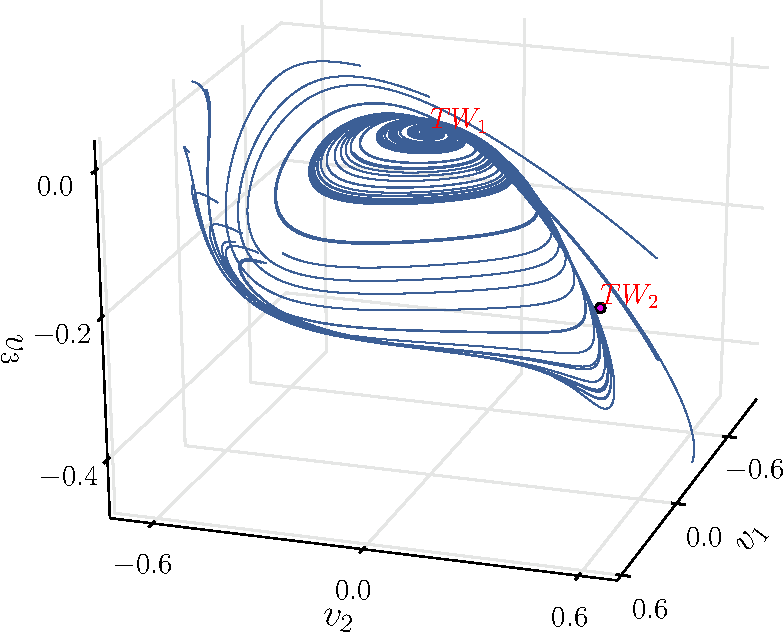
\includegraphics[width=0.45\textwidth]{BudCvi-ksssp} \,
 {(b)} 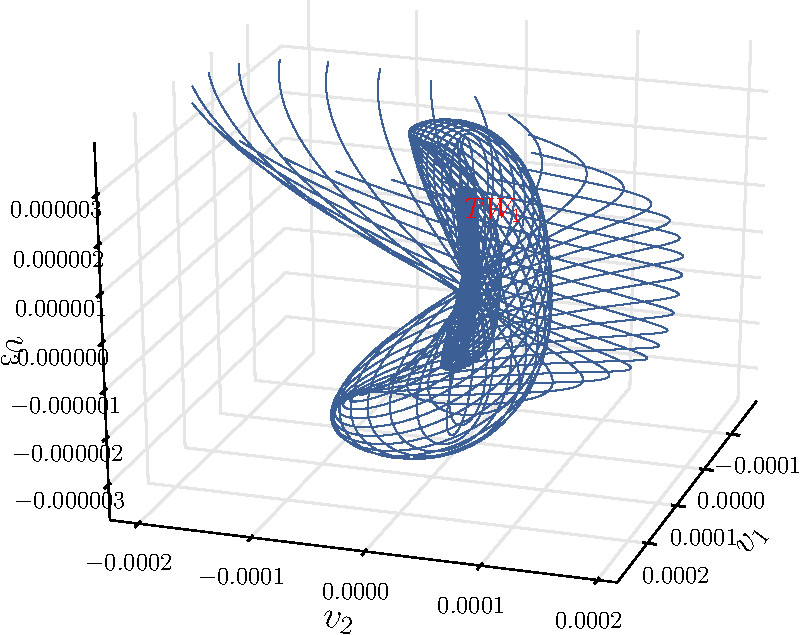
\includegraphics[width=0.45\textwidth]{BBkstwsspshort}
\end{center}
\caption{
(a) Unstable manifold of $\REQV{\pm}{1}$ in the reduced \statesp\ projection
traced out by integrating uniformly distributed initial points on a small
circle in the leading (complex) eigenvectors  $\jEigvec[1,2]$  plane
around the $\REQV{\pm}{1}$, for $t=120$. $(v_1,v_2,v_3)$ is the basis
set \refeq{eq-basisTW1}, with  $\REQV{\pm}{1}$ as the origin.
\Reqva\ $\REQV{\pm}{1}$ and $\REQV{\pm}{2}$ are marked with
red labels. (b) The same manifold plotted for $t = 43.5$.
}
\label{f-ksTWunstable}
\end{figure}
I solved \KS\ equation in the reduced state space with $20$ equally separated
initial conditions and projected onto the basis $(v_1, v_2, v_3)$. \refFig{f-ksTWunstable}
shows these $20$ orbits for $t=120$ (a) and $t=43.5$ (b). I plotted the shorter
orbit to see why there were thick curves separated by some distances on
\reffig{f-ksTWunstable}\,(a). We see on \reffig{f-ksTWunstable}\,(b) that the
trajectories starts on the same circle on $(v_1,v_2)$ plane, and expand in
every three direction (much faster in $v_1$ and $v_2$ directions, as expected,
see the axis scales in \reffig{f-ksTWunstable}\,(b)), while still being on
the surface of some kind of a torus. The thick regions (perhaps better seen
on a rotatable figure) in \reffig{f-ksTWunstable}\,(a) corresponds to the
surface of this torus which I think stays stable until trajectories come
closer to the second \reqv\ $\REQV{\pm}{2}$.

Sources for \reffig{f-ksTWunstable} are in \texttt{../figSrc/budanur/slice-f-ks}
see \texttt{00ReadMe} for which part does what.

\item[2014-03-16 Burak to Greg] I created the folder \texttt{../ksConnected/}
to store the \texttt{Matlab} code for $\SOn{2}$ reduced \KS\ system.
\texttt{00ReadMe} lists files and their functions. Solvers \texttt{ksETDRK4.m}
and \texttt{ksETDRK4red.m} could still have Matlab incompatibility issues,
Let me know if you get stuck on using any of these functions.
As far as I remember, you needed the velocity function (\texttt{velred.m})
and the \stabmat\  (\texttt{gradVred.m}); they are there and they should
run well on Matlab. I also added \texttt{tw.m} simply to store the \reqva\
on the slice.

\item[2014-03-16 Predrag to comrades NBB and XD]
Maybe you are ready to appreciate
the \emph{\HREF{http://www.chaosbook.org/projects/Siminos/thesis.pdf}
           {Thesis that Nobody Reads}}. Use the boyscout version in
this repository, there is much stuff there that did not make it into the
thesis. In particular, we tied ourselves in knots computing the stability
matrix in the slice, see sect.~4.2.3 \emph{Flotsam}, sect.~4.2.7
\emph{Stability of relative equilibria}, and the rest of the chapter is
not quite wrong either.

Today I started editing Xiong Ding's version,
\\
\texttt{Sym.tex} in \texttt{lyapunov/blog.tex},
\\
in hope that we will finally write down a compact and pretty version of
the in-slice stability matrices and \rpo\ Floquet matrices (these were
your problem sets that did not quite click last year).

For the record, we did know about 2.1.5 \emph{Principal fibre bundles}
back in 2008, but made editorial decision that the language is too
off-putting to a plumber on the street.

\item[2014-03-25 Burak] The unstable manifold \reffig{f-ksTWunstable}
had the initial conditions at the $\REQV{\pm}{1}$ which had components
in the third direction as well. However, after correcting that, I still see
band-like accumulation of trajectories on the $\REQV{\pm}{1}$
unstable manifold.
\\
\texttt{siminos/ksConnected/TWmanifold.m}
\\
 is a Matlab code that starts with
a $30$-dimensional initial guess for the $\REQV{\pm}{1}$ and it refines it by running
a Newton solver and then computes reduced stability eigenvalues and eigenvectors
for this point and integrates the system for $N$ different initial conditions
placed uniformly around a small circle \refeq{e-TWman_init},
 $\epsilon = 10^{-6}$.
        \PC{2014-03-26 unless you record things which were key to our
        discussions, it is not possible for other people to understand
        what is going on (or us, 3 months later). Please enter a table of
        numerical stability exponents, and for \reffig{f-ksTWunstable6L},
        continued fractions for the ratios numerical values}

\SFIG{ksTW1manshort}{}{
$10$ trajectories initiated uniformly along a infinitesimal circle
of radius $\epsilon = 10^{-6}$
in the unstable manifold plane of the leading eigenvector $\REQV{\pm}{1,2}$.
\KS\ system with
$L=22$, integrated for $t=30$.
}{f-ksTW1manshort}

If the imaginary parts of the leading eigenvalues are close to a
resonance, that can have a significant effect, which is presumably what
we see. These are not numerical errors; the circle radius $\epsilon = 10^{-6}$
is 4 orders of magnitude greater than our numerical accuracy
$\approx 10^{10}$. \refFig{f-ksTW1manshort} shows the $t=30$ evolution of
circle of uniformly distributed initial points in the $\REQV{\pm}{1}$
unstable manifold. We see a shape that looks like nested bottles. It is
this structure that `bands' the density of trajectories exiting the small
circle of initial conditions. from the structure of the `bottle' in
\refeq{f-ksTW1manshort}, and
    \PC{2014-03-26 please enter numerical value of $\epsilon$ in
    \reffig{f-ksTW1manshort}}
Note the scale of axes, while $e_1 \mbox{and}
e_2$ have values on the order $10^{-5}$, $e_3$ is on the order $10^{-9}$;
the \reqv\ that we are using is accurate
to the order $10^{-10}$). Now when we look at the ratio of imaginary parts of
the first 2 expanding eigenvalues, we get $\Im[\lambda_1]/\Im[\lambda_2] = 1.9509920$
(stored in the ratio variable in \texttt{TWmanifold.m}), with the continuous
fraction expansion $a_i = {1, 1, 19, ...}$. The larger $a_3$, the closer are
we to a resonance. If  $a_3=1$, we are on golden mean sequence, furthest from
a resonance, and expect no `banding' of initial conditions.

\begin{figure}
\begin{center}
 {(a)} 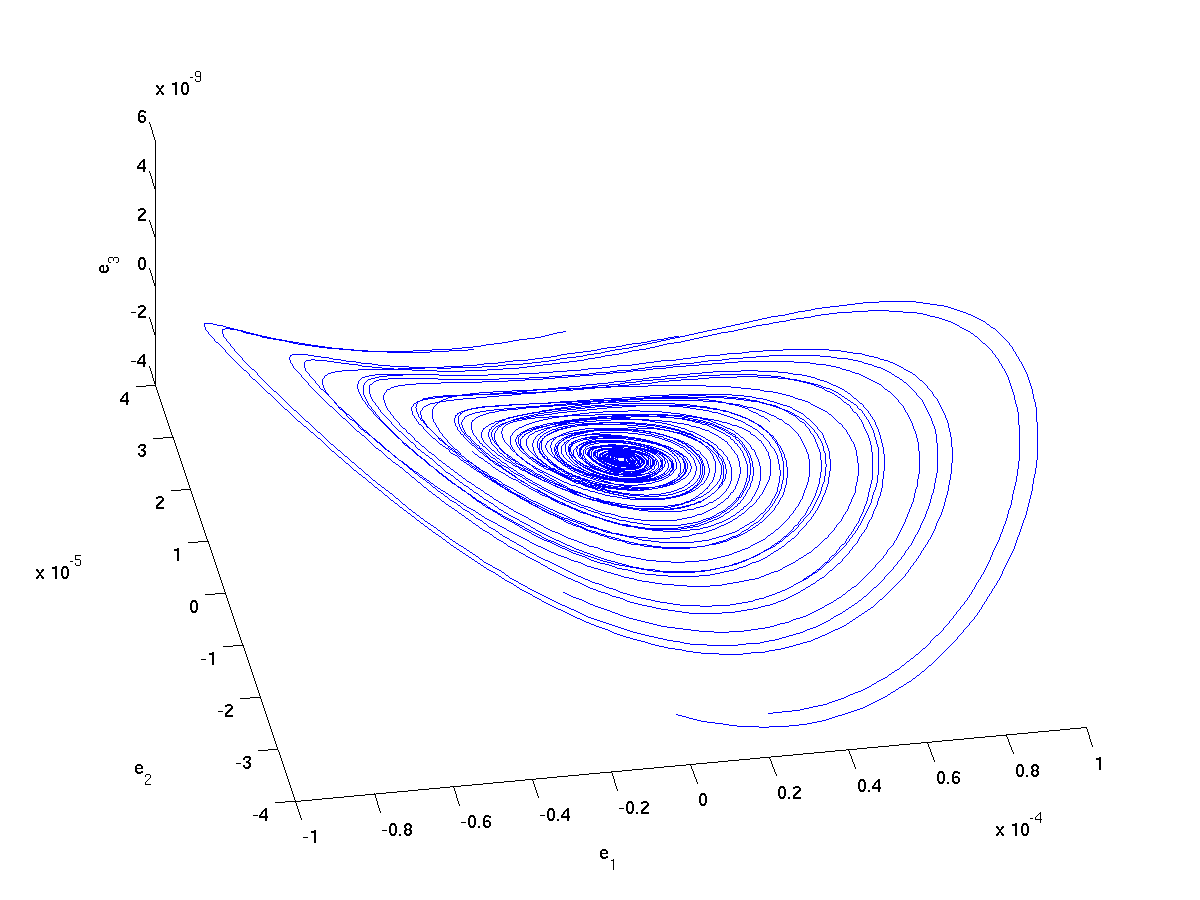
\includegraphics[width=0.25\textwidth]{ksTWmanL19} \,
 {(b)} 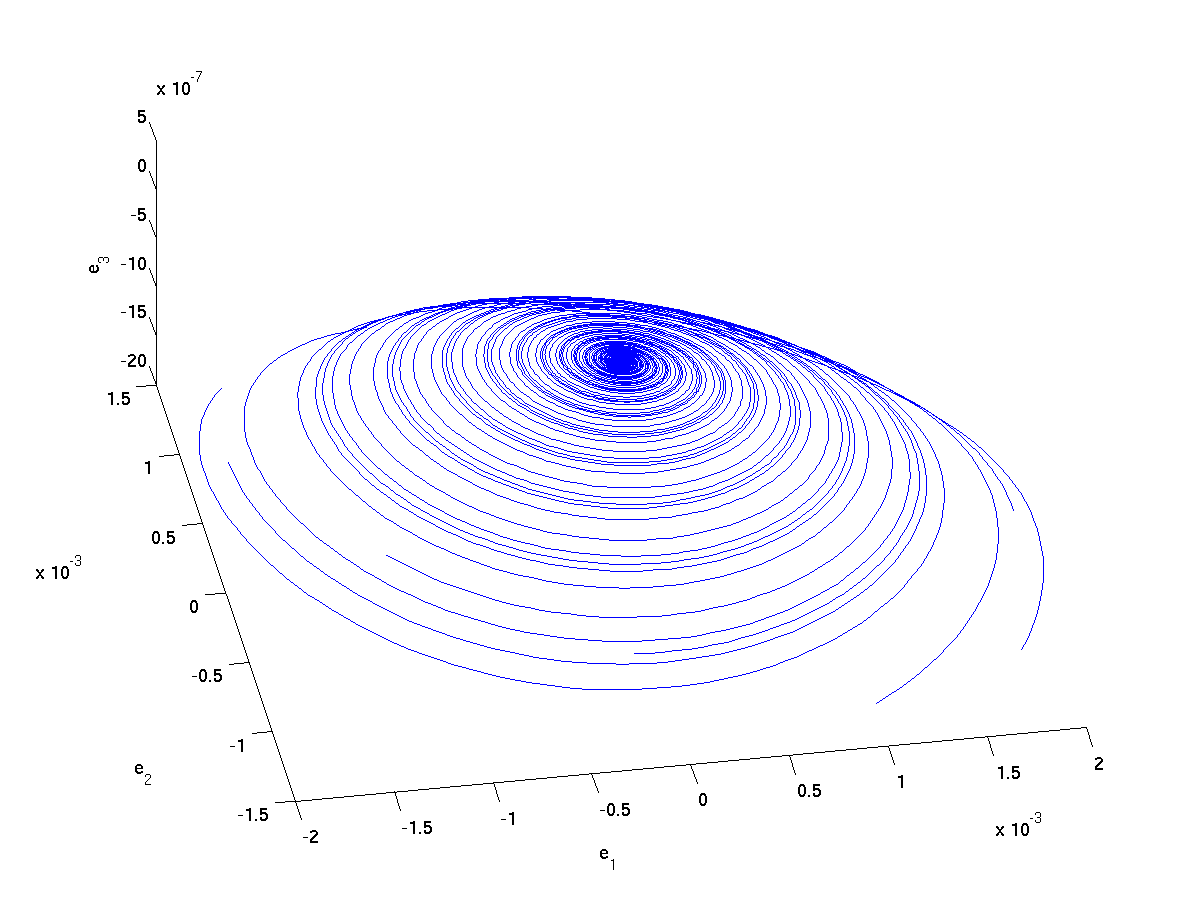
\includegraphics[width=0.25\textwidth]{ksTWmanL20} \,
 {(c)} 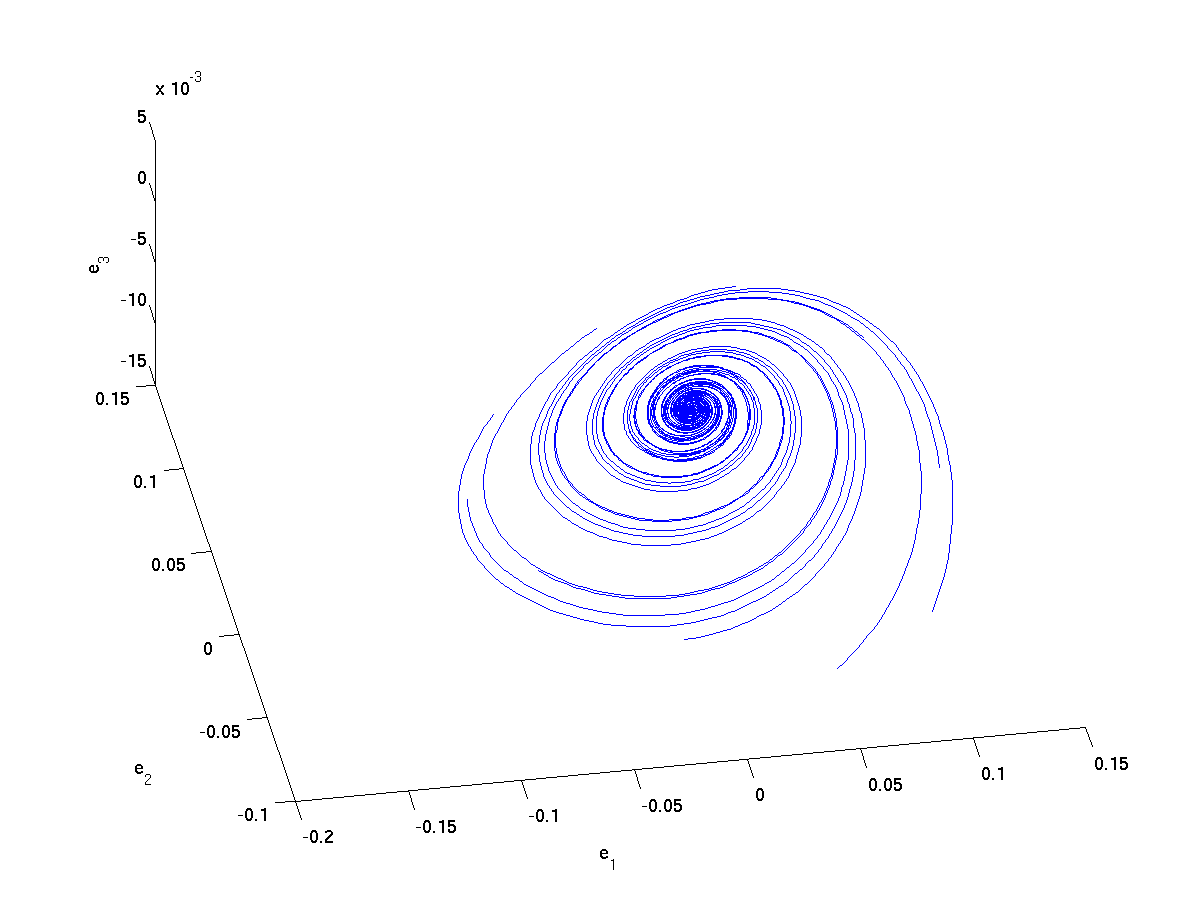
\includegraphics[width=0.25\textwidth]{ksTWmanL21} \\
 {(d)} 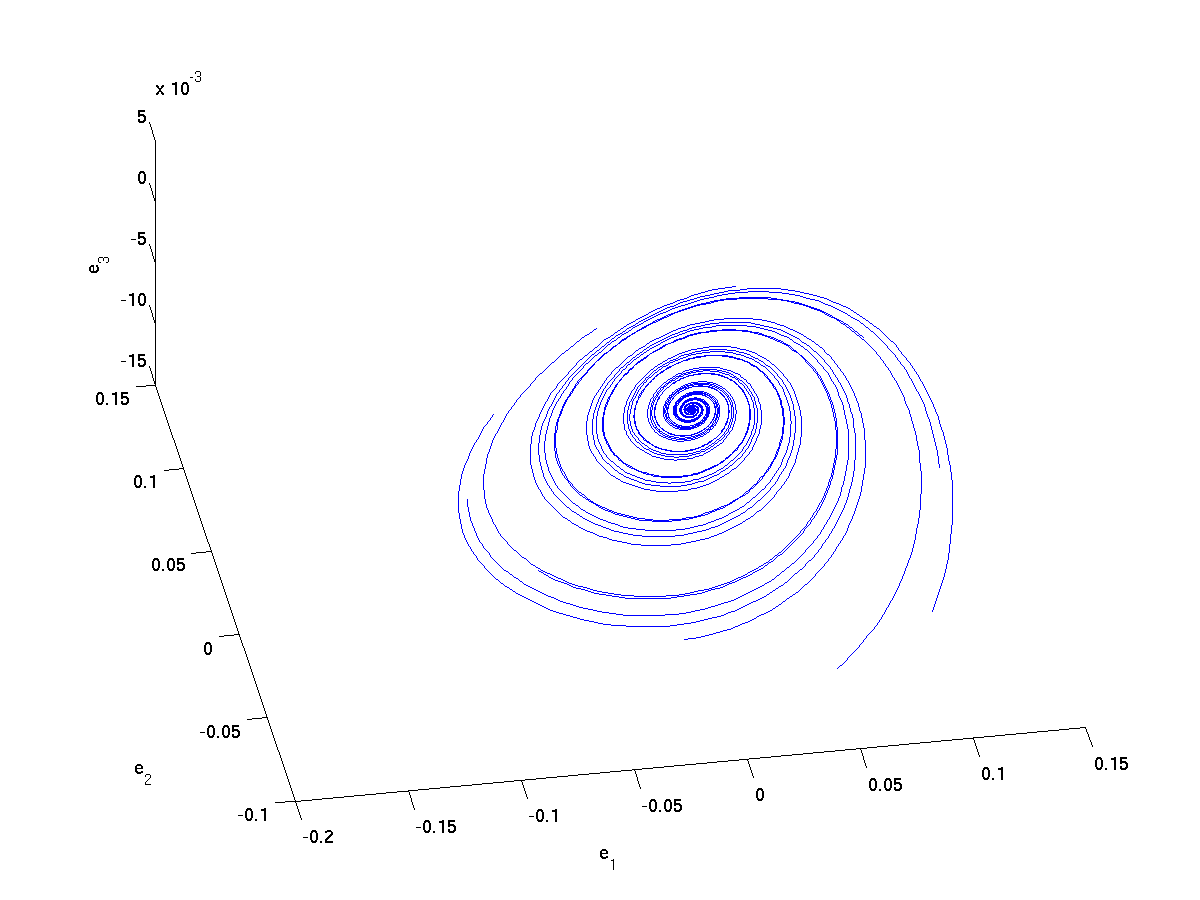
\includegraphics[width=0.25\textwidth]{ksTWmanL22} \,
 {(e)} 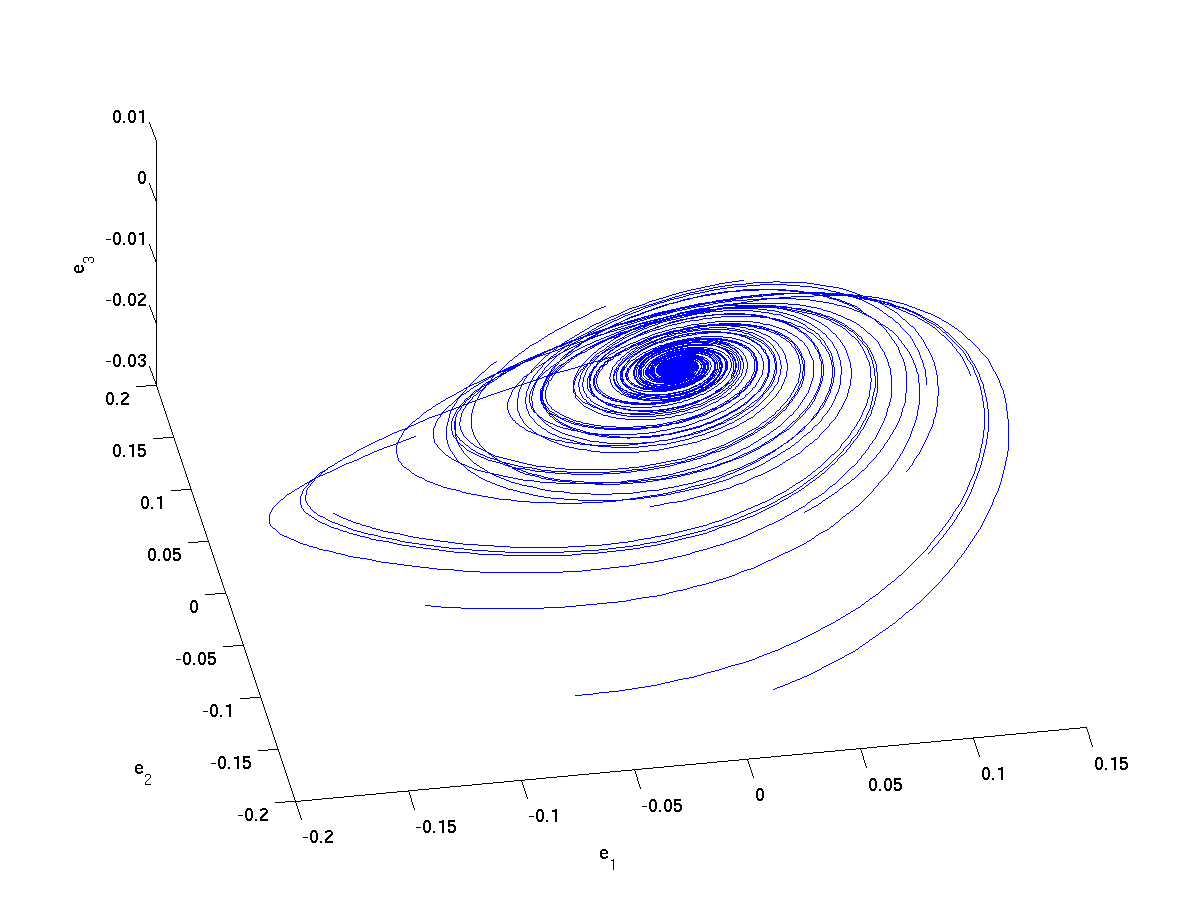
\includegraphics[width=0.25\textwidth]{ksTWmanL23} \,
 {(f)} 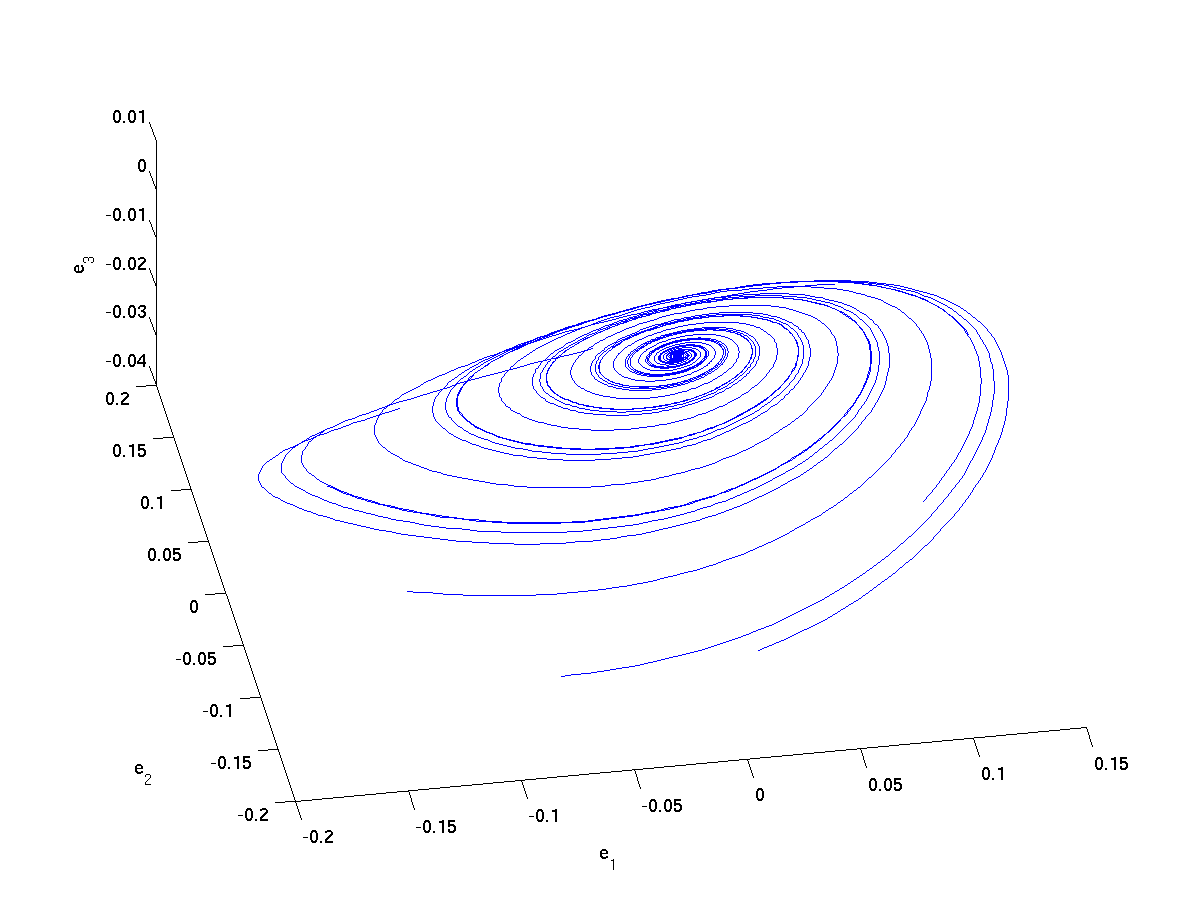
\includegraphics[width=0.25\textwidth]{ksTWmanL24} \,
\end{center}
\caption{
Unstable manifold of $\REQV{\pm}{1}$ in the \statesp\ projection computed
by integrating small perturbations around the $\REQV{\pm}{1}$ for $t=60$
For six different system sizes:
$L = 19, a_i = {1, 1, 12, 2,...} \mbox{(a)},
L = 20, a_i = {1, 1, 5, 1,...} \mbox{(b)},
L = 21, a_i = {1, 1, 9, 7,...} \mbox{(c)},
L = 22, a_i = {1, 1, 9, 7,...} \mbox{(d)},
L = 23, a_i = {1, 1, 157, 4, ...} \mbox{(e)},
L = 24, a_i = {2, 51, 4, 2, ...} \mbox{(f)}$.
$a_i$ is the continued fraction expansion of $\omega_1 / \omega_2$ for $L=20...24$
and $\omega_1 / \omega_7$ for $L=19$.
$(v_1, v_2, v_3)$ are the bases \refeq{eq-basisTW1}. }
\label{f-ksTWunstable6L}
\end{figure}

We can change the system size to explore the
effect of
this near resonance. To check that, I ran the same simulation with different
system sizes, in \reffig{f-ksTWunstable6L} there are $6$ different $L$
unstable
manifolds computed for $t = 60$. The ``bands''
change dramatically with the change in the system size. The ratios of the
imaginary part of the eigenvalues are all close to $2$, but their continued
fraction expansion vary a lot.
    \PC{2014-03-26 please enter continued fraction expansions, `close'
    is not helpful in this context.}
For $L=19$, the
unstable manifold starts to look like a saddle; this, I think, is because
for $L=22$, the third direction is no longer unstable, hence we have a resonance
between a stable and unstable eigenvalue.

While there still can be errors in my code that I'm not aware of, some basic
checks indicates that it is fine: My reduced \statesp\ integrator provides
outputs consistent with the full \statesp\ simulations (see figures in the slice
article), so I believe the integrator works well. While second suspect is
the \stabmat\ formula \refeq{e-stabMatRed}, frequencies of the spirals in the
unstable manifold are consistent with the eigenvalues of the stability matrix
and also it has a $0$-eigenvalue eigenvector along the symmetry direction,
so it also passes the sanity checks.

{\bf Question to Ruslan:} Do you have an idea about what we have here?

\item[2014-03-25 Ruslan]  I think the problem is with your initial
condition \refeq{e-TWman_init}.   See Section 5.1 in \rf{SCD07}.
You are using (5.2), while I think you should be using (5.1).

\item[2016-1-28 Xiong]

The knot structure in \reffig{f-ksTW1manshort}
could may be numerical issue because the
1st pair of eigenvectors may has some component of
the 2nd pair of eigenvectors. After different time to
reach \PoincSec, they have different expansion
in the direction of the 2nd pair. For short time,
the effect of 2nd pair will not vanish. Also non-linearity
may take effect also.
Anyway, it is hard for me to believe that it is due to
resonance.

\item[2014-03-25 Burak] Thanks! When I use radial initial conditions:
\beq
  \sspRed_0 = \sspRed_{TW} + \epsilon e^{\delta} e_1 \,
  \mbox{where} \, \delta \in [0, 2 \pi \mu / \nu ] \,
\label{e-TWman_init2}
\eeq
trajectories do look uniformly distributed. In \reffig{f-ksTWman119140},
I plotted outputs of unstable manifold calculations for $t=119$ (a) and $t=140$ (b).
In the latter, trajectories become turbulent and make close passages to the
\slicePlane\ border which we show with red color. In this projection, we
see the manifold has two layers.

\begin{figure}
\begin{center}
 {(a)} 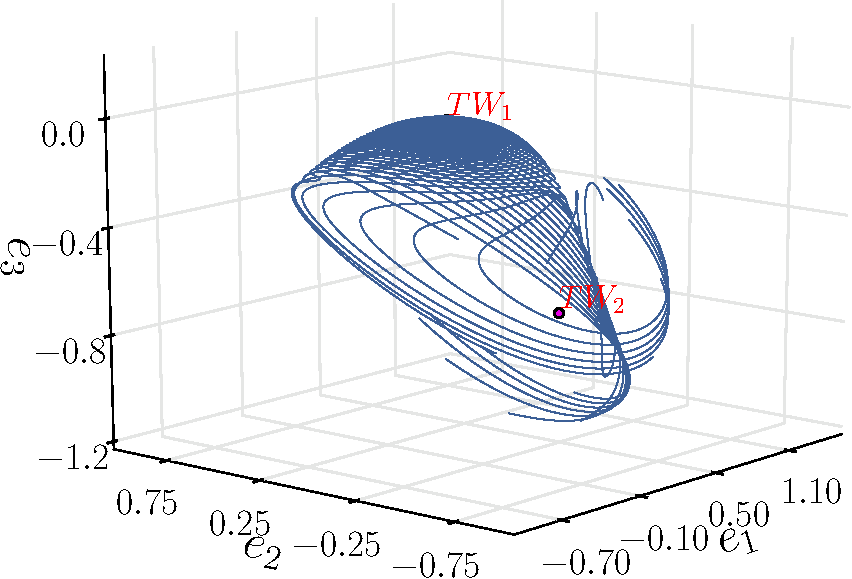
\includegraphics[width=0.45\textwidth]{ksTWman119} \,
 {(b)} 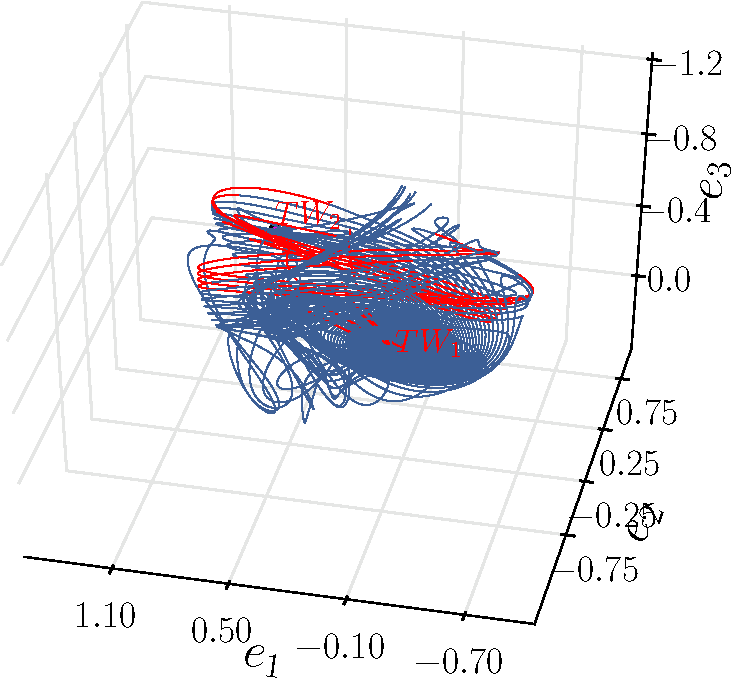
\includegraphics[width=0.45\textwidth]{ksTWman140}
\end{center}
\caption{ (a) Unstable manifold of $\REQV{\pm}{1}$ in the
reduced \statesp\ projection computed
by integrating a set of initial
conditions \refeq{e-TWman_init2} separated radially
from $\REQV{\pm}{1}$, for $t=119$.
(b) Same unstable manifold for
a longer time, $t=140$, where the close passages to the \slicePlane\
border ($a_1 < 0.05$) are indicated in red.
$(v_1, v_2, v_3)$ are the basis set \refeq{eq-basisTW1}
}
\label{f-ksTWman119140}
\end{figure}

Looking at \reffig{f-ksTWman119140}, we thought that computing the stable
manifold of $TW_2$ can provide some insight and we can may be manage to find
\hec s between travelling waves. However, my attempts to
compute the stable manifold so far was unsuccessful.

{\bf to Ruslan and Predrag} We should decide on symmetry reduced \KS\ figures
for the slice paper.
My opinion: I think the ones currently are there (3 Fourier mode projections
and configuration space plots) illustrates the method well. I know that Predrag
hates the Fourier mode projections, however, I think we should keep them to
show the turns during the close passages to the border. Regarding manifolds,
I think we can leave them to another publication since there are so many
things (\hec s, \PoincSec s etc.) to investigate
about them.

Let me know if there are other visualizations that you would like to see
so that I can generate them and we can compare and decide.

\item[2014-03-26 Predrag]
Evangelos had plotted the first-Fourier mode slice \rpo s together with
the unstable manifolds of \REQV{\pm}{1} and \EQV{2} in
\reffig{fig-2009-08-29TW1} (I have seen the same
plot on Burak's screen). Please use conventions of \refref{SCD07}, in
particular number the eigenvalues in the same way. I have copied
\reftab{tab:Eksym} to the blog, as a reminder.

\begin{table}%[t]
\caption{
Leading eigenvalues
$\eigExp[j]= \eigRe[j] \pm i\eigIm[j]$
and symmetries of the corresponding eigenvectors of KS {\eqva} and
\reqva\ for $L = 22$ system size.
We have used as our reference states the ones that lie within the
antisymmetric subspace  $\bbU^+$, and also listed the symmetries of the
$L/4$ translated ones.
        }\label{tab:Eksym}
\begin{center}
    {\footnotesize
\begin{tabular}{ccccc}
\EQV{1}& $\eigRe[j]$ & $\eigIm[j]$ & Symmetry & $\Shift_{1/4}\EQV{n}$ Symmetry\\\hline
  $\eigExp[1,2]$ & $\ \ 0.1308$& $0.3341$ & -  & -\\
  $\eigExp[3,4]$ & $\ \ 0.0824$& $0.3402$ & $\bbU^+$  & $\bbU^{(1)}$\\
  $\eigExp[5]$   & $0$     &          & -  & -\\
  $\eigExp[6,7]$ &$-0.2287$& $0.1963$ & $\bbU^+$  & $\bbU^{(1)}$\\
  $\eigExp[8]$   &$-0.2455$&          & -  & -\\
  $\eigExp[9]$   &$-2.0554$&          & $\bbU^+$  & $\bbU^{(1)}$\\
  $\eigExp[10]$  &$-2.0619$&          & -  & -\\[2ex]
\EQV{2}&  &  & \\\hline
  $\eigExp[1,2]$ & $\ \ 0.1390$& $0.2384$ & $\bbU^+$         & $\bbU^{(1)}$\\
  $\eigExp[3]$   & $0$      &          & $\Shift_{1/2}$        & $\Shift_{1/2}$\\
  $\eigExp[4,5]$ &$-0.0840$ & $0.1602$ & $\bbU^{(1)}$           & $\bbU^+$\\
  $\eigExp[6]$   &$-0.1194$ &          & $\Shift_{1/2}$        & $\Shift_{1/2}$\\
  $\eigExp[7,8]$ &$-0.2711$ & $0.3563$ & $\bbU^+,\,\bbU^{(1)},\,\Shift_{1/2}$  & $\bbU^+,\,\bbU^{(1)},\,\Shift_{1/2}$\\
  $\eigExp[9]$   &$-2.0130$ &          & $\bbU^{(1)}$           & $\bbU^+$\\
  $\eigExp[10]$  &$-2.0378$ &          & $\bbU^+$         & $\bbU^{(1)}$\\[2ex]
\EQV{3}&  &  & \\\hline
  $\eigExp[1]$   &$\ \ 0.0933$&          & $\bbU^+$     & $\bbU^{(1)}$\\
  $\eigExp[2]$   &$\ \ 0.0933$&          & -         & -  \\
  $\eigExp[3]$   &$0$       &          & $\Shift_{1/3}$    & $\Shift_{1/3}$\\
  $\eigExp[4]$   &$-0.4128$ &          & $\bbU^+,\,\Shift_{1/3}$  & $\bbU^{(1)},\,\Shift_{1/3}$\\
  $\eigExp[5,6]$ &$-0.6108$ & $0.3759$ & $\bbU^+$     & $\bbU^{(1)}$\\
  $\eigExp[7,8]$ &$-0.6108$ & $0.3759$ & -         & -\\
  $\eigExp[9]$   &$-1.6641$ &          & -         & -\\
  $\eigExp[10]$  &$-1.6641$ &          & $\bbU^+$     & $\bbU^{(1)}$ \\[2ex]
$\REQV{\pm}{1}$&  &  & \\\hline
  $\eigExp[1,2]$ & $\ \ 0.1156$ & $0.8173$ & -  & -\\
  $\eigExp[3,4]$ & $\ \ 0.0337$ & $0.4189$ & -  & -\\
  $\eigExp[5]$   & $0$      &          & -  & -\\
  $\eigExp[6]$   &$-0.2457$ &          & -  & -\\
  $\eigExp[7,8]$ &$-0.3213$ & $0.9813$ & -  & -\\[2ex]
$\REQV{\pm}{2}$&  &  & \\\hline
  $\eigExp[1]  $ & $\ \ 0.3370$ &          & -  & -\\
  $\eigExp[2]  $ & $0$      &          & -  & -\\
  $\eigExp[3,4]$ &$-0.0096$ & $0.6288$ & -  & -\\
  $\eigExp[5,6]$ &$-0.2619$ & $0.5591$ & -  & -\\
  $\eigExp[7,8]$ &$-0.3067$ & $0.0725$ & -  & -\\
\end{tabular}
    } %end    {\footnotesize
\end{center}
\end{table}

\item[2014-03-26 Predrag to Burak] I'm confused - when we talked about
it, did you tell me that the near resonance is between the slowest
\emph{contracting} complex eigenpair and the fastest expanding eigenpair.
I must have heard you wrong, as I do not see that in the
\reftab{tab:Eksym}. Did you only mean $L=19?$

\item[2014-03-26 Burak] Yes, I said that only for $L=19$, for the rest, near
resonance is between first and second expanding eigenvalue. I posted stability
eigenvalues in \reftab{t-tw1evals}

\begin{table}%[t]
\caption{
Leading eigenvalues
$\eigExp[j]= \eigRe[j] \pm i\eigIm[j]$
of the \KS\ \reqv\ ($TW_1$).
Eigenvalues with non zero imaginary parts have a corresponding complex
conjugate, which we omitted in this table.
        }\label{t-tw1evals}

\begin{tabular}{ccc}
$L = 19$ & $L=20$ & $L=21$   \\
\begin{tabular}{cc} $\mu_i$ & $\omega_i$ \end{tabular} &
\begin{tabular}{cc} $\mu_i$ & $\omega_i$ \end{tabular} &
\begin{tabular}{cc} $\mu_i$ & $\omega_i$ \end{tabular} \\
\input{../ksConnected/data/lambdatexL19} &
\input{../ksConnected/data/lambdatexL20} &
\input{../ksConnected/data/lambdatexL21}
\end{tabular}

\begin{tabular}{ccc}
$L = 22$ & $L=23$ & $L=24$   \\
\begin{tabular}{cc} $\mu_i$ & $\omega_i$ \end{tabular} &
\begin{tabular}{cc} $\mu_i$ & $\omega_i$ \end{tabular} &
\begin{tabular}{cc} $\mu_i$ & $\omega_i$ \end{tabular} \\
\input{../ksConnected/data/lambdatexL22} &
\input{../ksConnected/data/lambdatexL23} &
\input{../ksConnected/data/lambdatexL24}
\end{tabular}
\end{table}

\item[2014-03-31 Burak]  In \refref{rowley_reduction_2003}, there is a formulation
of \mslices\ that uses a time rescaling transformation (see eq. 9). I tried
to understand what that meant but the paper is a bit too mathematical for
me, so if you have a look and see whether if it is equivalent to the time
rescaling that we do, that would be nice. Either way, we need to cite them
in the slice paper. They scale by $m(g)$ and they say it is a homomorphism
of Lie groups and my brain blue screens.

\item[2014-04-02 Burak to Predrag and Ruslan] I finished my edits on the
slice article today. I think it is ready to go on arxiv, please have a look
at it, especially names and addresses, I copied Ruslan's from \texttt{ksReduced.tex}.
Let me know if you think that I should change a figure.

\item[2014-04-11 Burak] I plotted the unstable manifold of the travelling
wave in the full \statesp\ next to the sliced manifold. We see in the full
\statesp , the drifts along the group orbit dominates the trajectories as
they spiral out from the travelling wave. I left the marks for the travelling
waves in the figure, they are of course just one points on their respective
group orbits, I can polish this figure, may be draw the entire group orbit
of the travelling waves if you think that we should include it in the slice
paper.

I also plotted configuration space evolution using the scaled time and added
to slides
\HREF{http://www.cns.gatech.edu/~burak/talks/slice/\#/23}{23},
\HREF{http://www.cns.gatech.edu/~burak/talks/slice/\#/24}{24},
\HREF{http://www.cns.gatech.edu/~burak/talks/slice/\#/25}{25}
of my web presentation. I think they do a nice job in illustrating how time
rescaling resolves the fast jumps well.

\begin{figure}
\begin{center}
 {(a)} 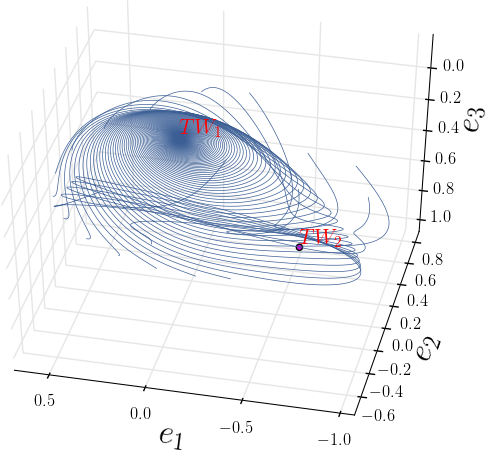
\includegraphics[width=0.45\textwidth]{kstwsspt120} \,
 {(b)} 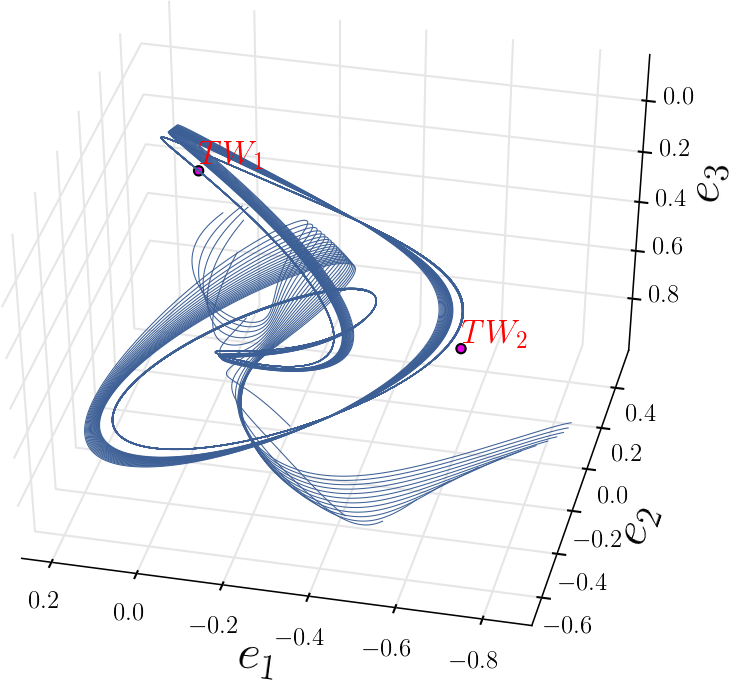
\includegraphics[width=0.45\textwidth]{kstwsspfullt120}
\end{center}
\caption{ (a) Unstable manifold of $\REQV{\pm}{1}$ in the
reduced \statesp\ projection computed
by integrating a set of initial
conditions \refeq{e-TWman_init2} separated radially
from $\REQV{\pm}{1}$, for $t=120$.
(b) Same unstable manifold in the full \statesp .
}
\label{f-kstwmansspredfull}
\end{figure}

\item[2014-04-15 Burak] To be able to compare different \rpo s, I wrote
a little Matlab program \texttt{../ksConnected/plotrpo.m} which loads \rpo\
initial conditions from Ruslan's solution database and integrates them in
equivariant and reduced \statesp s and plots outputs side by side. By
changing the rpo number in 9th and 10th lines of the code, you can plot it
for any rpo in the solution db. After looking at a few, I found $RPO_{33.5010}$
most informative as in the \statesp\ projection (\reffig{f-KSrpo335010ssp})
initial and final points of the trajectory are far from each other, although
connected by the group action, in the it becomes a periodic orbit. I found
configuration space plots \reffig{f-KSrpo335010conf} particularly useful
in illustrating the importance of the time-rescaling since the abrupt jumps
in the physical time are indeed very well resolved in the time-rescaled plot.


\begin{figure}
\begin{center}
 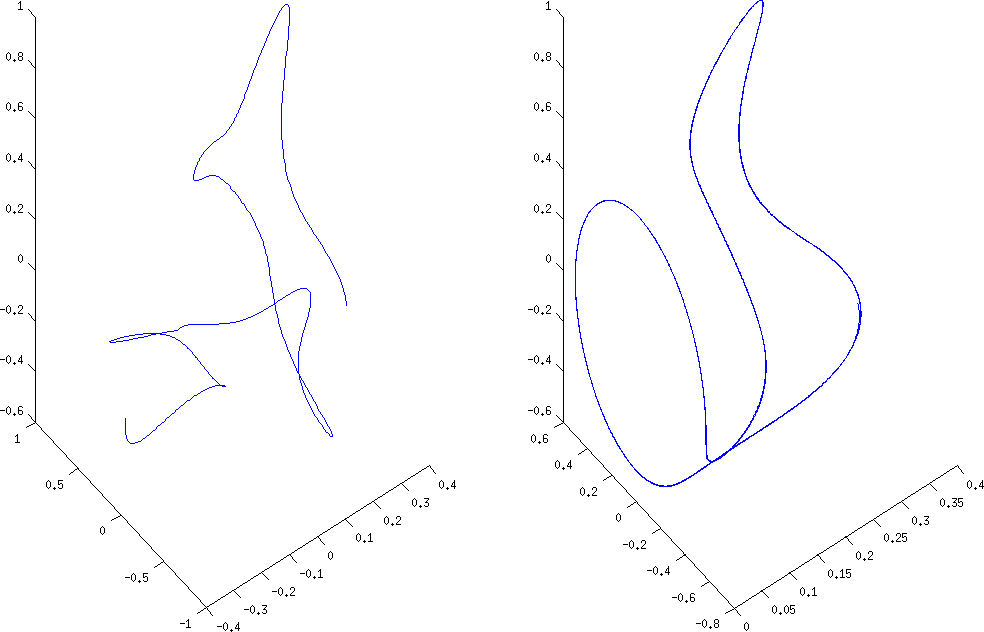
\includegraphics[width=0.90\textwidth]{KSrpo335010ssp} \,
\end{center}
\caption{ 3 Fourier mode projection of the \KS $RPO_{33.5010}$ in
full \statesp\ (left) and on the \slicePlane\ (right).
}
\label{f-KSrpo335010ssp}
\end{figure}

%\begin{figure}
%\begin{center}
% 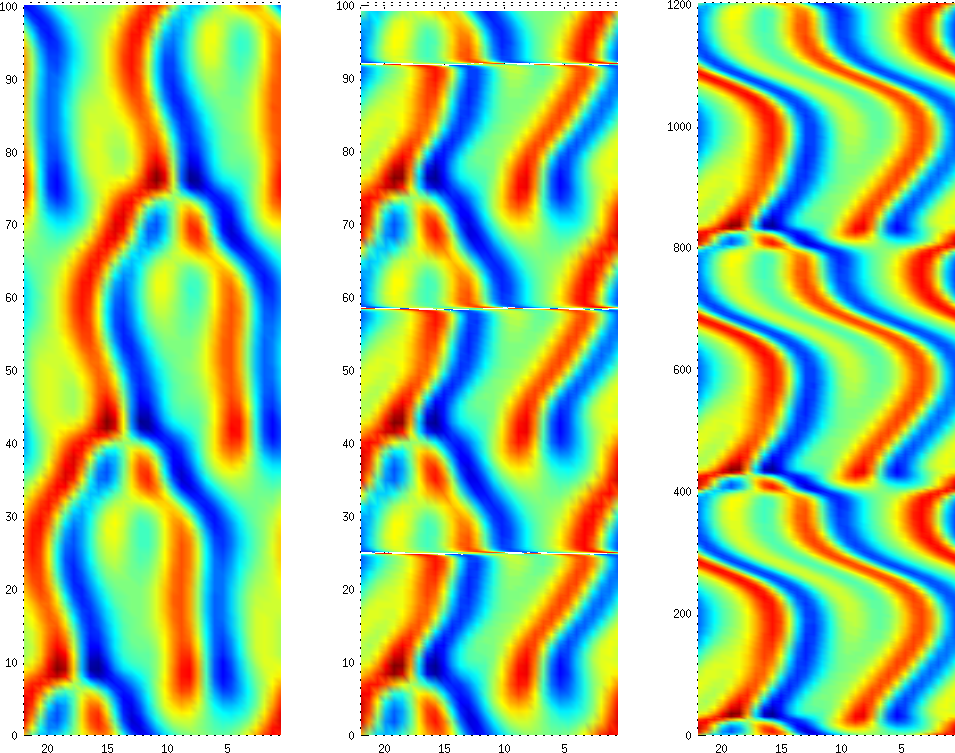
\includegraphics[width=0.90\textwidth]{KSrpo335010conf} \,
%\end{center}
%\caption{ Configuration space plots of the \KS $\RPO{33.50}$:
% (a) Without
%symmetry reduction. (b) Symmetry reduced evolution in time $\zeit$
%exhibits fast phase changes when the 1-st Fourier mode is small.
%(c) Symmetry reduced evolution in slice time $\hat{\zeit}$
%is smooth for all $\hat{\zeit}$.
%}
%\label{f-KSrpo335010conf}
%\end{figure}

\item[2014-04-15 Predrag]
%\refFig{f-KSrpo335010conf} is a good illustration of evolution in the
%slice time $\hat{\tau}$ vs. the time $\tau$
I've changed $t \to \tau$ to
avoid confusion with the group tangent.
Do not call $\tau$ `physical
time, and do not label figures with text - that goes into caption (a), (b)
(c) - not (left), (middle), (right). Always trim figures (no white frame).
\BBedit{Burak: I added low quality figures stick together with unintelligible
ticks just to give you a quick example so that you can share your opinions
about which figures to include in the slice article. I won't do it again
if this is unacceptably low quality for the blog, it's just practical.}

Instead of Fourier modes in \reffig{f-KSrpo335010ssp}, use \statesp\ projection
with enough repeats of the \rpo\ so its torus can be seen, such as
Fig.~1.
\HREF{http://www.cns.gatech.edu/~predrag/papers/ACHKW11.pdf}{here}.

\item[2014-04-15 Burak]
As requested by Predrag, I used the following basis to project the state space
solution onto:
\bea
   e_1 &=& \Lg \ssp_0 / |\Lg \ssp_0| \continue
   e_2 &=& \Lg^2 \ssp_0 / |\Lg^2 \ssp_0|  \continue
   e_3 &=& (\sspRed_d - \sspRed_0 )_{\perp} / |(\sspRed_d - \sspRed_0 )_{\perp}|
   \label{e-ksrpobasis}
\eea
where $\ssp_0 = \sspRed_0$ is the initial point on the \rpo , and $\sspRed_d$
is the furthest point from $\sspRed_0$ on its symmetry reduced orbit and
the subscript $\perp$ indicates that this vector is gone through Gramm-Schmidt
orthogonalization. This projection looks like \reffig{f-KSrpo335010FS}.
I didn't find this particularly illuminating but I may be ignorant to its
beauty. For the slice paper, my opinion is that we can only show the configuration
space plots along with the ones plotted with respect to slice time, I think
they will be enough for the purpose of illustrating the first mode slice.

\begin{figure}
\begin{center}
 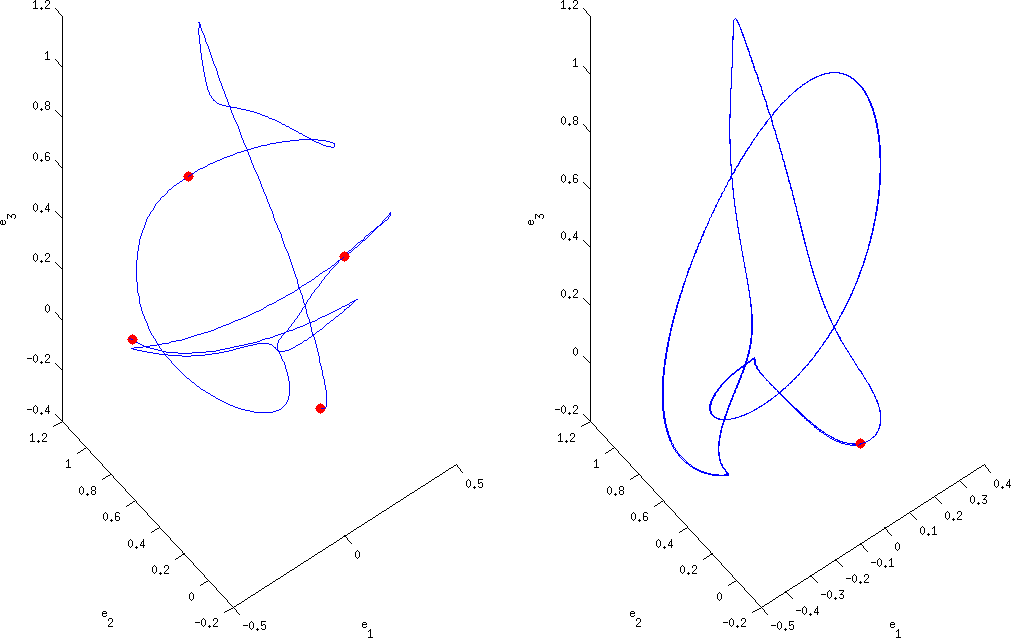
\includegraphics[width=0.90\textwidth]{KSrpo335010FS} \,
\end{center}
\caption{ \KS $RPO_{33.5010}$ integrated for 3 periods projected onto
the basis \refeq{e-ksrpobasis} in full \statesp\ (left) and on the
\slicePlane\ (right).
}
\label{f-KSrpo335010FS}
\end{figure}

\item[2014-04-15 Predrag to Evangelos] I'm happy to step aside as a
co-author of \refref{BudCvi14} (where I have contributed nothing but
complaints) as long as you firmly commit to leading the collaboration and
completing \refref{SCD09b}.

\item[2014-04-28 Evangelos to Predrag] I do not understand this at all, isn't
complaining the main responsibility of an advisor? Now more seriously, it would
be totally unacceptable that you left \refref{BudCvi14} and I do not see
any reason in doing this. I will propose a different deal that, I think, has some
added value in it. Since I have started working again on the problem,
I will keep going, and blog here. If you find something useful that falls
within the scope of \refref{BudCvi14} and you would like to incorporate it
into it, then you may reconsider adding me as co-author.

\item[2014-04-28 Evangelos] In the following I will try to show why, eventhough
I had used first Fourier mode slice as starting point for symmetry reduction,
I am not completely happy with it. At least one of the difficulties,
related to slicing the unstable manifold of $E_2$ has now been resolved,
see below.

\item[2014-04-28 Evangelos] In order to illustrate what stopped us from making
progress with first Fourier mode slice, I copy here Ruslan's plots from
[2011-11-21 Ruslan], see \reffig{f:KS22E2man1_copy}.
Ruslan applies a first Fourier mode slice in order to
visualize the unstable manifold of \EQV{2}. However trajectories on this
manifold lie on the antisymmetric subspace and therefore have purely imaginary
Fourier coefficients. Then, it is natural to expect that trajectories on this
manifold will intersect the chart border, when $y_1$ changes sign. Indeed such
intersections do occur and we get a figure like \reffig{f:KS22E2man1_copy}(b),
which looks like a manifold cut in half.

\item[2014-04-28 Evangelos]
This might not sound important, but we have good reasons to believe that many of
KS relative periodic orbits (and in particular \RPO{33.5010}),
are still organized by this unstable manifold, even though they leave in full space.
In turn such relative periodic orbits seem to be important organizing blocks of
the spatiotemporaly chaotic dynamics of KS. The most common pattern we see is an
interplay between second and third Fourier mode, and this is exactly what happens
in the neighborhood of the unstable manifold of \EQV{2}.

\begin{figure}[ht]
\begin{center}
(a)~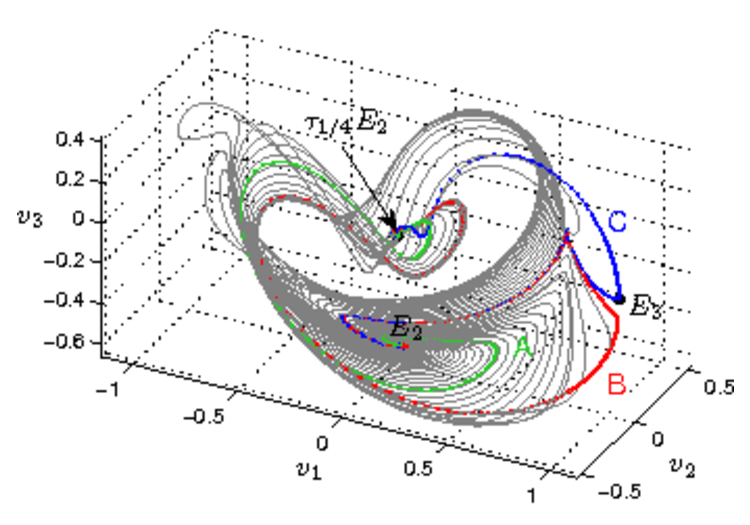
\includegraphics[width=0.48\textwidth, clip=true]{ks22_E2_manifold_c}~
(b)~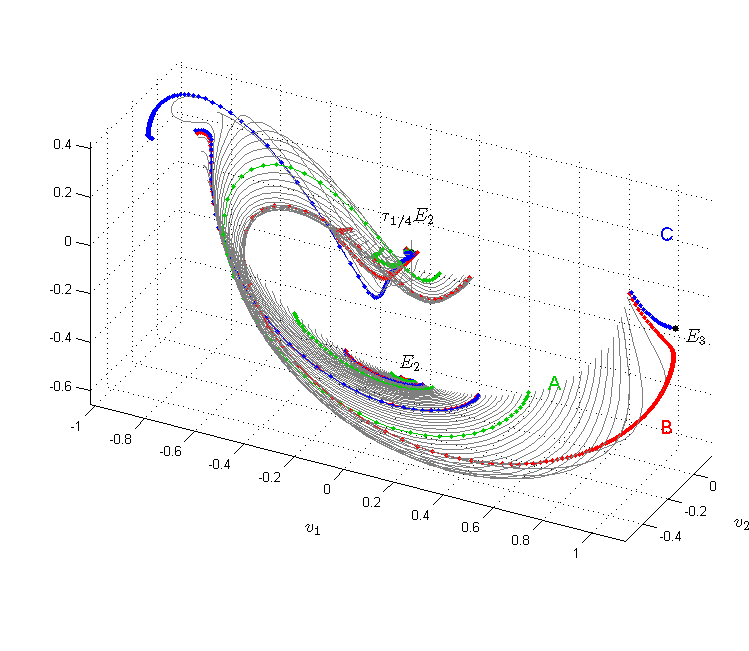
\includegraphics[width=0.48\textwidth, clip=true]{ks22_E2_MSO2_manifold}
\end{center}
\caption{
(a) The two-dimensional unstable manifold of \eqv\
\EQV{2}, from \refref{SCD07}. (b) {\bf 2011-11-18 Ruslan}
two-dimensional unstable manifold of \eqv\ \EQV{2} in
$\pS/\SOn{2}$ slice at $\theta_1 = \pi/2$. The coordinate axes $v_1$,
$v_2$, and $v_3$ are constructed from vectors Re\,$\jEigvec[1]$,
Im\,$\jEigvec[1]$, and {Re\,}$\jEigvec[7]$ by Gram-Schmidt
orthogonalization.
       }
\label{f:KS22E2man1_copy}
\end{figure}

\item[2014-04-28 Evangelos] I did hope initially that the time-rescaled
integration would help bring the two halfs of \reffig{f:KS22E2man1_copy}(b)
together, but unfortunately the crossing of the charter border is genuine here,
so rescaled integration will stagnate.

However, all phase jumps in \reffig{f:KS22E2man1_copy}(b) are by $\pm\pi$, so
in countless discussions in this blog we said there should be
a systematic way to remove them, but never did this. I do not know why I had not thought
of this until last week, but there are systematic ways to ``unwrap'' phase jumps
(by $2\pi$) in signal processing, \eg, Itoh's algorithm\cite{itoh82}. Therefore,
one can integrate \EQV{2} unstable manifold trajectories (in full space),
then fix a slice by $c_1=0$ (for example), record the timeseries of angles $\theta_i$
that maps each point onto the slice, apply phase unwrapping to remove discontinuities
in $\theta_i$, and then apply the rotation that maps each point on the slice.
The result is shown in \reffig{f:KS22E2man1_unwrapped}. The unstable manifold
now has the appearance it should have.

There is still a nuisance associated to the close visits to the neighborhood of
the translated copy of $\EQV{2}$ through its stable manifold. I think what happens
here is that as the trajectory approaches $\tau_{1/4}\EQV{2}$ at some point the phase in the
$a_1$ plane is really dominated by roundoff error. This should be removable by
integrating in rescaled time (on the slice) or by stopping integration soon enough
before reaching $\tau_{1/4}\EQV{2}$. Unfortunately, it is a general feature of first
mode slice that $\EQV{2}$ and $\EQV{3}$ do not lie on it. However, their
position is fixed by their stable/unstable manifolds, so when it comes to studying
topology of the attractor, I think there is no problem. It is also annoying that
$\EQV{2}$ and $\tau_{1/4}\EQV{2}$ are not identified in \reffig{f:KS22E2man1_unwrapped}(a)
(and the same for $\EQV{3}$), but I hope there are no practical consequences.

In retrospect, the unstable manifold of \EQV{2} is a very special object, in that it
can be brought onto the slice by a rotation by a constant angle (here, I think,
by $\pi/2$). The main point of the exercise is that this is done self-consistently,
by demanding continuity of $\theta_i$.

Note that while there are $\pi$ jumps when we cross the chart border in antisymmetric
subspace, Burak has shown that there no such jumps for
generic trajectories when using the first mode slice in full phase space (by
the probabilistic argument, there are no chart border crossings and $\theta$
varies sharply but continuously)
\ES{I wonder if we may play the same trick of applying a discrete symmetry
transformation to remove phase jumps for trajectories in full space
that hit the chart border for general templates.
I try with the two-modes system and CLE for now.
}.

\begin{figure}[ht]
\begin{center}
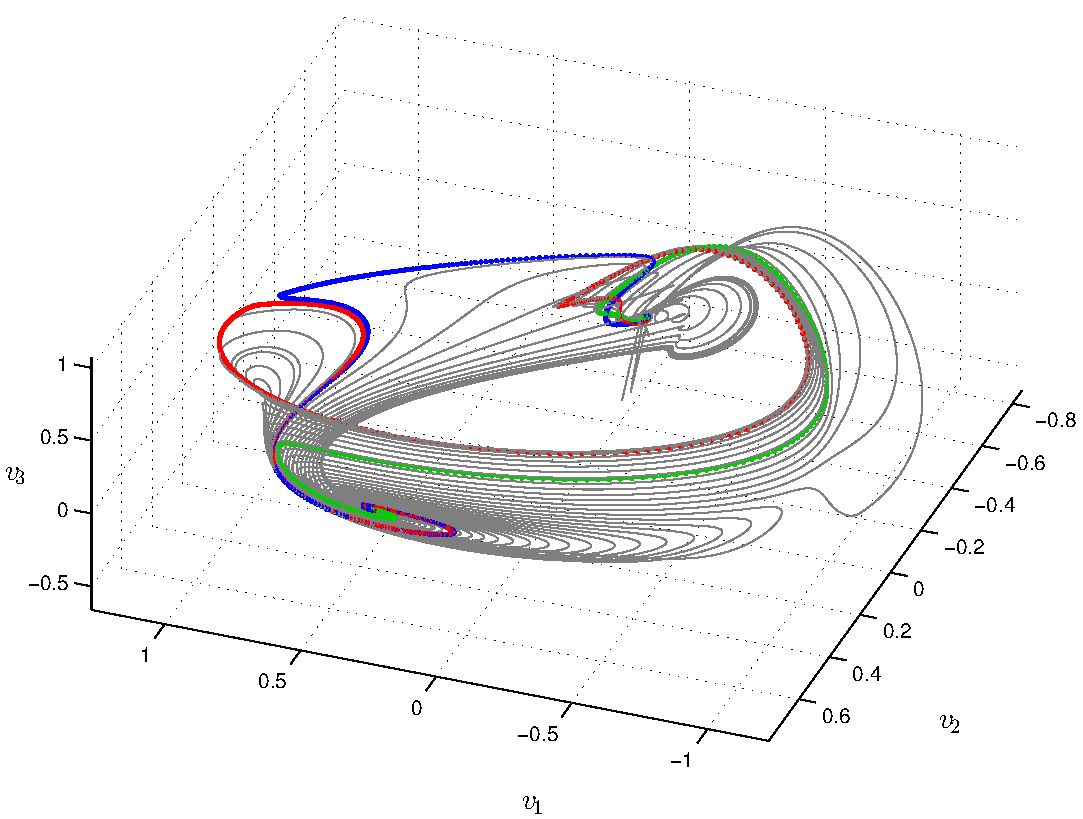
\includegraphics[width=0.48\textwidth, clip=true]{ks22_E2_manifold_inv_mf1}
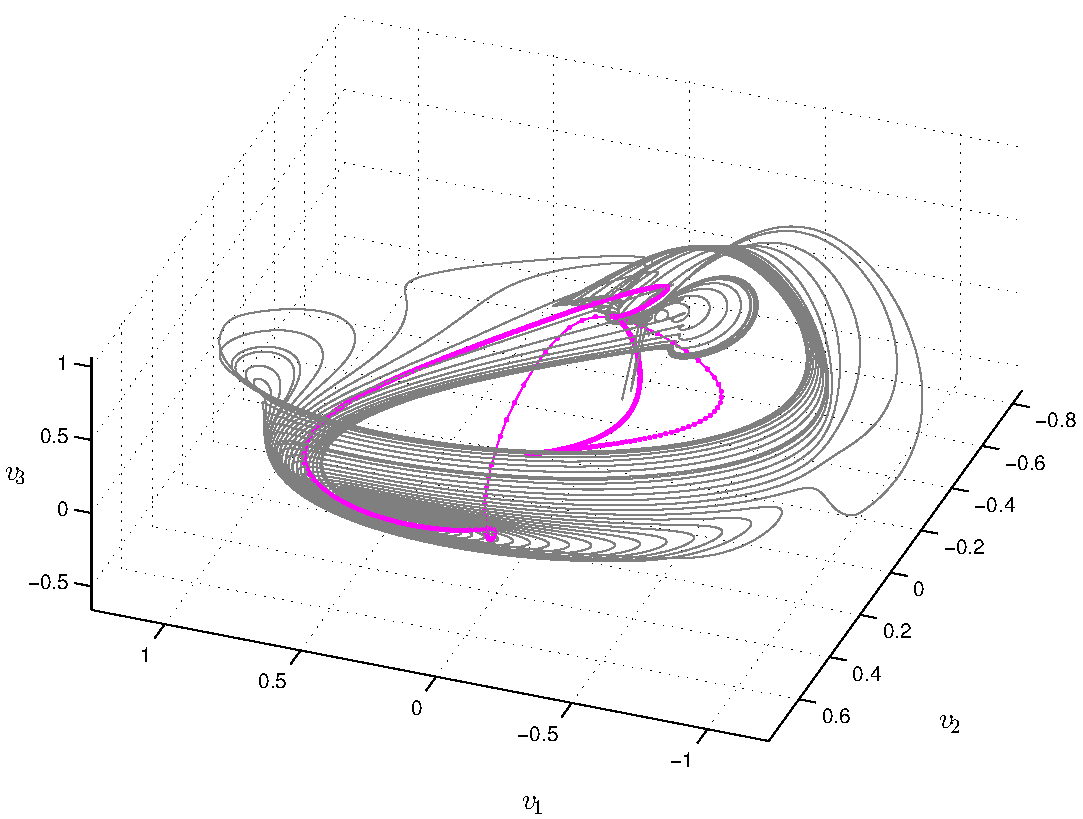
\includegraphics[width=0.48\textwidth, clip=true]{ks22_E2_RPO33p5_manifold_inv_mf1}
\end{center}
\caption{
(a) Unstable manifold of \eqv\ \EQV{2}, on the slice defined by $c_1=0$,
constructed by applying moving frame transformations after unwrapping
the phase variable. (b) Same as in panel (a), but also with \rpo\ \RPO{33.5} (magenta).
The coordinate axes $v_1$, $v_2$, and $v_3$ are constructed from vectors Re\,$\jEigvec[1]$,
Im\,$\jEigvec[1]$, and {Re\,}$\jEigvec[7]$ by Gram-Schmidt
orthogonalization.
       }
\label{f:KS22E2man1_unwrapped}
\end{figure}

\item[Evangelos 2014-04-28] Having the unstable manifold of \EQV{2} back in one piece,
we can now plot along it \RPO{33.5}, as in \reffig{f:KS22E2man1_unwrapped}.
Note that here I do not integrate on the slice, everything is done
by postprocessing. I just use sufficiently many points along the orbit so that there is
no visible discontinuity on the slice.

I think that this figure suggests that the unstable manifold of \EQV{2}
plays indeed a role in the dynamics of \RPO{33.5}. Some of the longer
relative periodic orbits stay close to the unstable manifold for longer
times.

By the way, if you would like to plot a \rpo\ which is organized by the unstable manifold of \REQV{}{1},
a good candidate is the shortest orbit $\RPO{1}=\RPO{16.32}$.

\item[Evangelos 2014-04-28] A problem with reviewers is that they always like to ask
how to choose a slice. In \refref{BudCvi14} you avoid providing a justification
for using the first Fourier mode slice, which I find fair enough, but you will certainly get
the question. Internally in this blog, there is an argument that I do not understand,
which is that only first Fourier mode slice will work. In \reffig{f:KS22TW1_manif_mf}, I give a
counterexample, in which also the {\sFslice} works for visualization of
the unstable manifold of \REQV{}{1} of KS.

\begin{figure}
\begin{center}
(a)~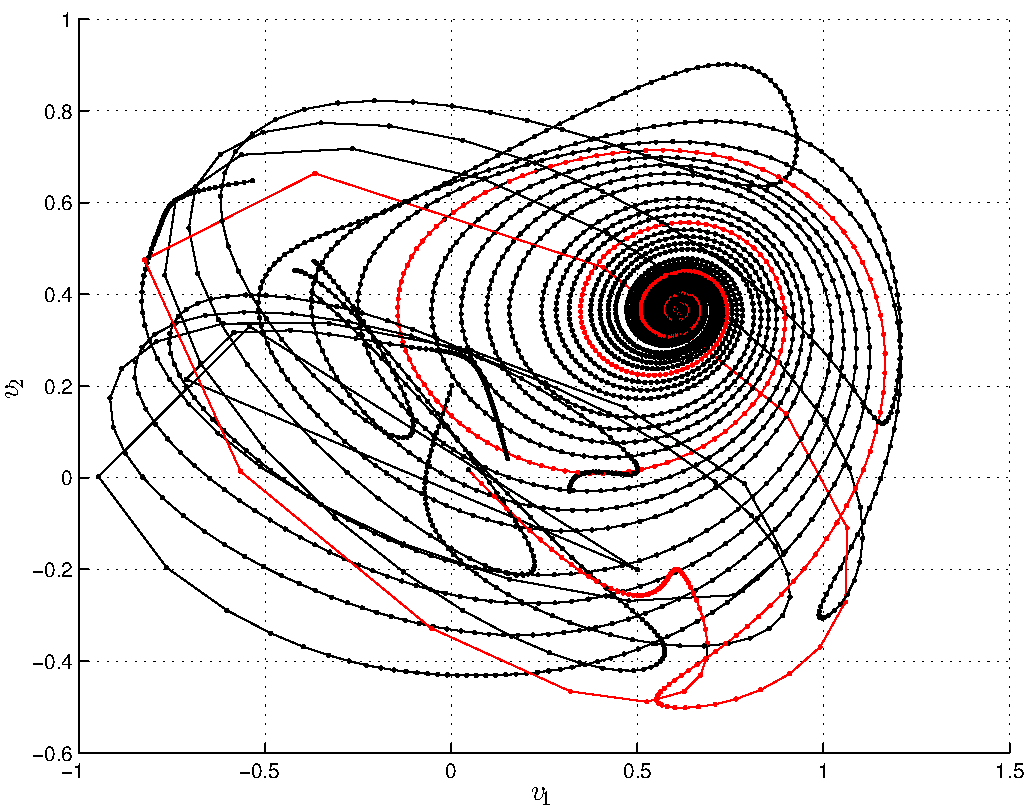
\includegraphics[width=0.45\textwidth, clip=true]{ks22_TW1_manif_inv_mf1}~
(c)~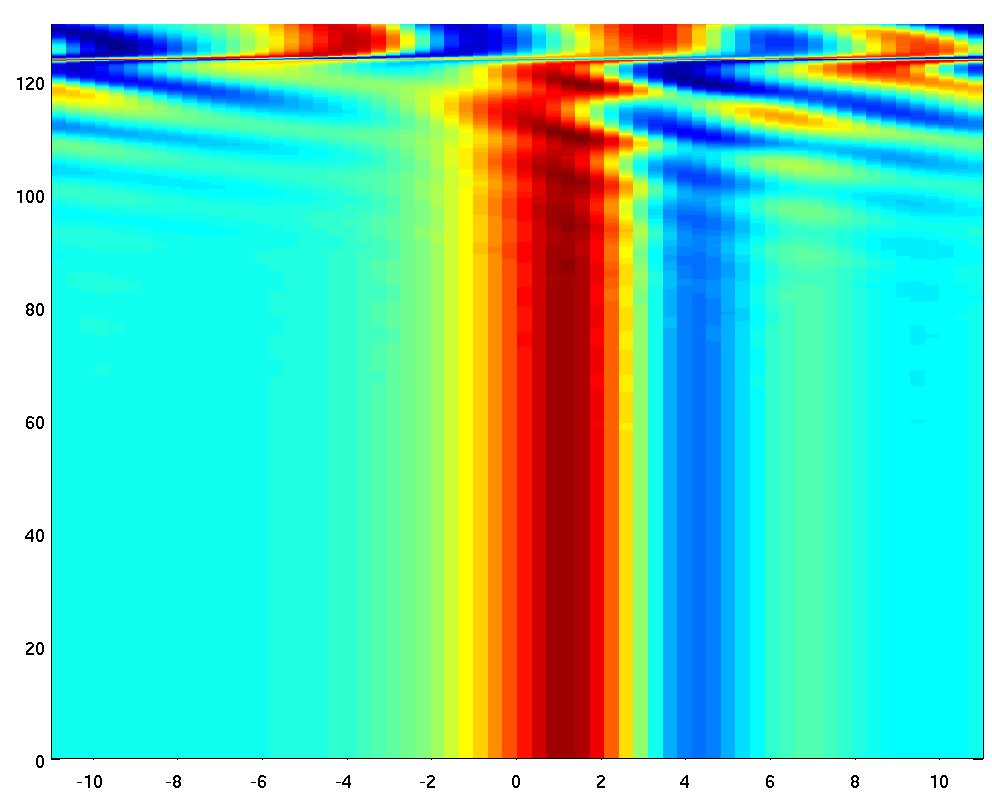
\includegraphics[width=0.20\textwidth, height=0.6\textwidth, clip=true]{ks22_TW1_traj_red_inv_mf1}\\
(b)~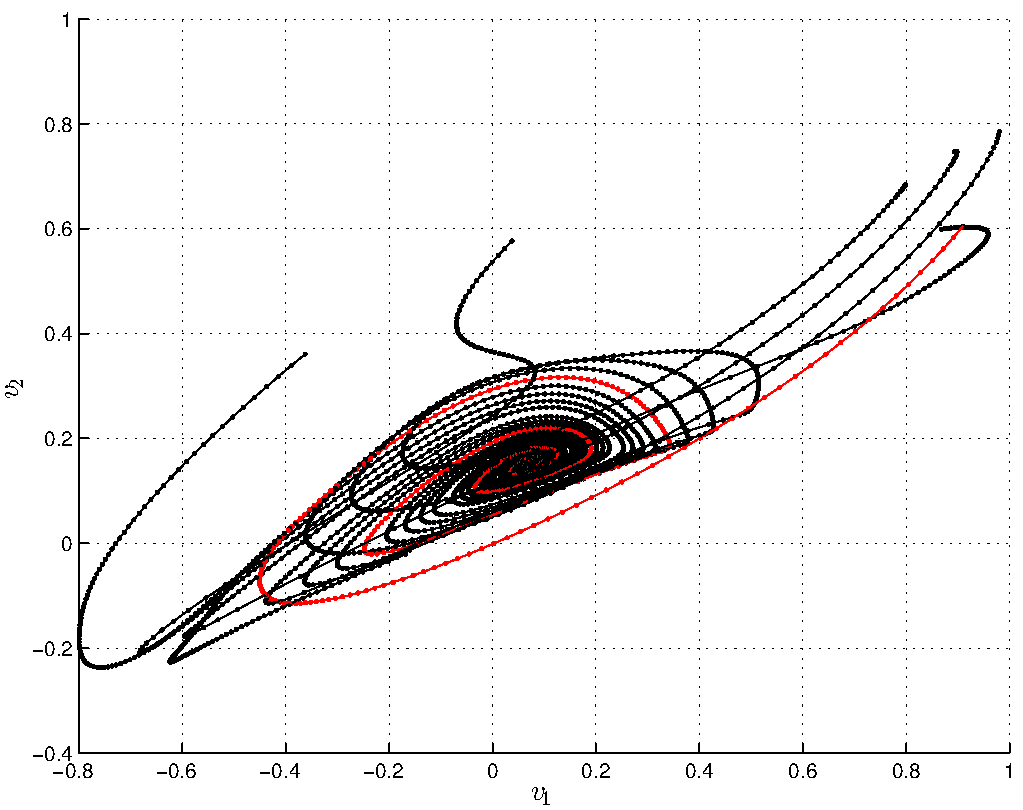
\includegraphics[width=0.45\textwidth, clip=true]{ks22_TW1_manif_inv_mf2}~
(d)~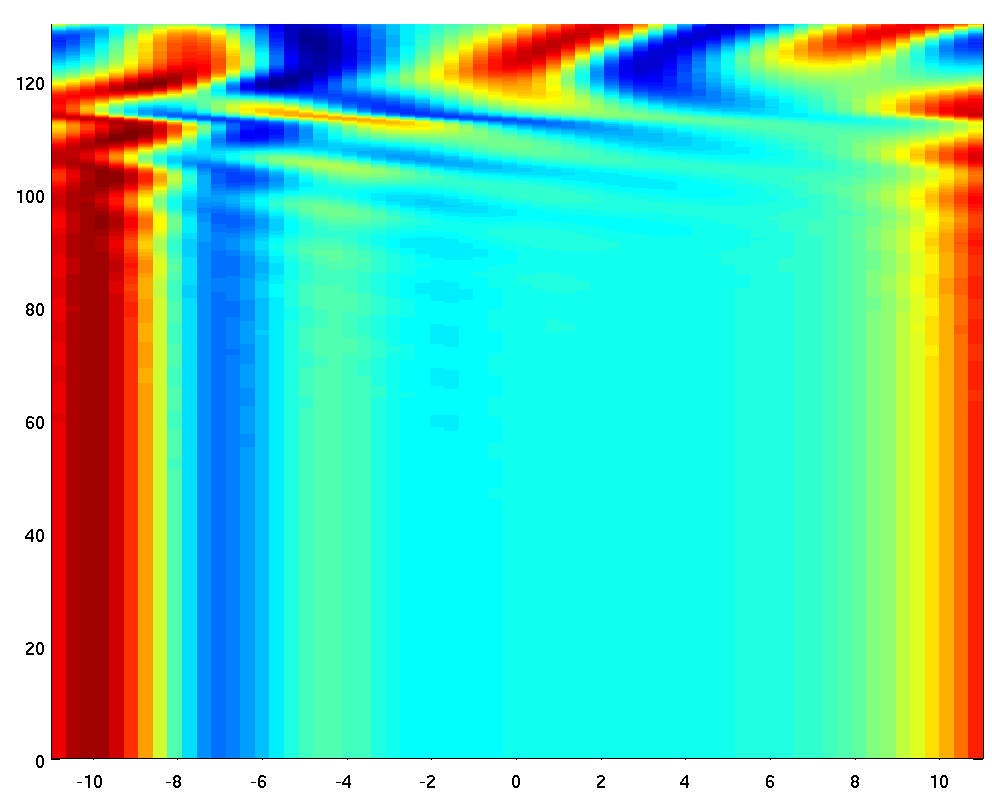
\includegraphics[width=0.20\textwidth, height=0.6\textwidth, clip=true]{ks22_TW1_traj_red_inv_mf2}
\end{center}
\caption{
(a) Unstable manifold of \reqv\ \REQV{}{1}, on the slice defined by $c_1=0$,
and (b) $c_2=0$. (c), (d) Colormap of $u(x,t)$ for the trajectory shown in
red in panel (a) and (b), respectively.
The coordinate axes $v_1$, $v_2$ are constructed from vectors Re\,$\jEigvec[1]$,
and Im\,$\jEigvec[1]$ by Gram-Schmidt
orthogonalization.
       }
\label{f:KS22TW1_manif_mf}
\end{figure}

Here I use the method of moving frames, \ie, I integrate in original space and then
map the (same) points on the two different slices (I integrate up to $t=130$, a bit
longer than in \refref{BudCvi14}).
I do not try to use a fine timestep, because I want to
compare the degree of smoothness of trajectories in the two slices.
You can see that using $c_2=0$ slice, one gets smoother trajectories, without large
jumps. Moreover there are no large jumps in the $u(x,t)$ space plots.

However, I would like to stress that {\sFslice} is not
panacea; if we integrate for longer time there will be "jumps", and we
would still need to employ time rescaling to overcome them. I have also
tried sixth mode slice which is quite interesting because you can then
also put \EQV{2} and \EQV{3} on your slice, and it still looks very
reasonable.

The points I am trying to make are the following: (1) I do not see something special
with first Fourier mode slice, compared with other single mode slices, but please
provide a counterexample if I am wrong. (2) Using {\sFslice} improves
things a bit because it is more relevant to KS physics than first mode: in KS we have
competition between two wave and three wave structures, in the neighborhood of
which $|a_1|$ likes to become small.

For me, if I take the dynamical systems point of view, any single mode slice (for which
the probabilistic argument holds) is OK. If you care about the attractor geometry or
topology, any sensible conjugacy is fine. I prefer to use first Fourier mode slice
because it's easier to derive analytical expressions for the transformations, but
from a computational viewpoint, I can see no difference.

However, if you would like to reach to fluid dynamicists or experimentalists,
then it's a different story. Then you might need to pay attention to the physics of
the problem at hand to motivate your slice. For instance, an experimentalist cannot
increase sampling rate as the flow approaches a chart border.

\renewcommand{\ssp}{a}

\item[Burak 2014-04-29] The confusion about the other modes is due to
the fact that $k^{th}$ mode transforms as $\ssp_k \rightarrow e^{i k \phi} \ssp_k$,
so the slice defined by $Im[\ssp_k] = 0, Re[\ssp_k] > 0$ is cut by the group orbits
by $k$ times for $\phi \in [0, 2 \pi)$. Regarding discussion in the slice paper
is the sentence in which we previously said ``This slice is cut by the group
orbits once and only once'' and Ruslan corrected us as ``only for the first
mode''. This being said, I don't think this is computationally a big issue
since this ambiguity can be easily resolved by defining the transformation
that brings modes to the \slice\ as:
\beq
   \sspRed_n \rightarrow e^{-i \phi_k} \ssp_n \, ,
\eeq
where $\phi_k$ is the phase of the \slice -fixing mode. In addition, I
think the reduced evolution equations will also be correct for $n^{th}$
mode slice.

I tried to reproduce your unstable manifold computation but I failed, probably
because of a stupid mistake, but I can't find it. However, \reffig{f:KS22E2man1_copy} (b)
confuses me, and I tend to think that there must be something wrong. My
reason is, when I compute the stability eigenvalues for $EQ_2$, I find that
the most expanding eigenvalue has non-zero first Fourier mode, which would
move the far from border, and then when they fall into the strange attractor,
competition between 2nd and 3rd Fourier mode should be resolved well with
the in-\slice\ integration with the \slice\ time. There may as well be
some other factor that I don't account for, because when I try to integrate
within the slice near to the $EQ_2$ in the most unstable direction (brought)
back into the slice, my integration failed, but currently I don't trust this
result because I also failed to generate the unstable manifold in the full
\statesp .
[ {\bf [ES 2014-05-02]} We could look at why your computation fails together.
Both me and Ruslan have computed the unstable manifold of \EQV{2} independently,
so we are pretty confident about this calculation. To begin with, you might want
to have a look in Ruslan's code in siminos/matlab/ruslan/kse22figs.m to see
what initial condition he uses.]


On the other hand, I also think that $2^{nd}$, $3^{rd}$ and/or $6^{th}$ Fourier
mode slices can be much more insightful in visualizing the unstable manifold
of $EQ_2$ and in general \KS\ dynamics since the important stuff really
is the competition between $2^{nd}$ and $3^{rd}$ modes and in the first mode
slice they both are in the border.

Another issue that I think we should consider here is that the initial perturbation
that we make to compute the unstable manifold is in the full \statesp ,
and I think we need compute stability within the slice if we want to have
a correct unstable manifold, which again something we cannot do on the first
mode slice since $EQ_2$ lies on the border. On the other hand, may be we
can derive a stability in terms of \slice\ time, and that would be finite
even on the border, and then we can use that for the computation of unstable
manifold of $EQ_2$.

Regarding contributions to the publications, my humble opinion is that Evangelos
has already helped significantly to the development of single-mode slicing
by being critical to it and proposing different, probably more useful, formulations
of it; so I think only good can come from joining forces.

\item[2014-04-15 Predrag to Evangelos]
Itoh's algorithm\rf{itoh82} wrapping (not unwrapping:)\ES{Itoh uses a
wrapping operator in order to unwrap wrapped phase. His algorithm is
known in signal processing as phase unwrapping (\ie, restoring
continuity).
Let's not be the only ones who call it the other way.} in
\reffig{f:KS22E2man1_unwrapped} is brilliant. Can you put the code
somewhere so Burak can turn this thing in 3D, it would be easier to
visualize. I also like \reffig{f:KS22E2man1_copy}\,(b), we can almost see
how the jumps work. It would be interesting to see explicitly how this
gets wrapped into \reffig{f:KS22E2man1_unwrapped} - perhaps by marking
\reffig{f:KS22E2man1_copy}\,(b) jump points on the wrapped unstable manifold?

Can you use Itoh's wrapping also for the 1. Fourier mode $\to 0+$ episodes?

{\bf [2014-04-15 Evangelos]} No, unfortunately for 1. Fourier mode outside
antisymmetric subspace, this trick is of no use.
The reason is that, as Burak has showed, there we have close visits but no transversals
of the chart border. Thus, the jumps do not correspond to a well defined
discrete symmetry operation ($\pm \pi$ shift as we thought).
Probably this is why we could not make such a
simple trick work for CLE.

But what I have also be trying is to see if Itoh's trick helps with general slices
whose chart border is pierced transversaly by the flow. I am trying this in
the two modes system. I think at the end it all amount to quotienting a discrete
symmetry artificially introduced by the slice crossings.

You can get the 3D figures in matlab by running the first ``cell'' of
file siminos/matlab/ruslan/ks22reduced.m. I hope I did not forget
to check in some subroutine.

\item[2014-04-15 Predrag to Evangelos] Will the copy of
\eqv\ $\tau_{1/4}$ \EQV{2} get identified with \EQV{2}\ once one
quotients out $\Dn{1}$?\ES{I need to reread our SIADS paper to answer this.}

Can the two copies of fundamental domain in \On{2}\ reductions (see
figures in Xiong Ding' s chapter of the \texttt{lyapunov/} blog, someplace
around \textbf{2014-02-28}) be tied seamlessly by a trick similar to
Itoh's? There it is not wrapping up of a phase translation, but the
reflection of all real parts of Fourier modes that causes the
discontinuities.

{\bf[2014-04-15 Evangelos]} I think yes, and that's why I brought this
up today. In general it should be possible to keep track of any discrete
symmetry operation and undo it.

\item[2014-04-30 Ruslan] Burak is right that using higher single Fourier modes
will not satisfy the uniqueness requirement for the slice.  But, as I mentioned before,
we can define a slice by fixing the difference between phases of consecutive modes,
$k$ and $k+1$, to recover the uniqueness.  We can use $k=2$.
The problem is that we will still see 'fast' changes within the slice whenever t
he magnitudes of either $k$-th or $(k+1)$-st mode become small.
There are probably other ways to have uniqueness.
Related to this: the way the slice is defined in the paper, I wonder if, in addition,
we should impose some condition on $\hat{a}^\prime$ which will guarantee the uniqueness.
Any ideas?

\item[2014-04-30 Burak] When we are defining the 1st mode slice we also
specify which half of the hyperplane we are using by saying slice is $\hat{x}_1 \geq 0$
on the slice. For the general hyperplane condition $\braket{\sspRed}{\sliceTan{}} = 0$
, we can also impose $\braket{\groupTan{(\sspRed})}{\sliceTan{}}>0$ to make
it unique but I don't think it's necessary on that part of the paper since
we make that issue clear in our slice choice.

\item[2014-04-30 Evangelos] Usually the uniqueness requirement is satisfied by requiring
that $\sspRed$ is a global minimum among the points
satisfying $\braket{\sspRed}{\sliceTan{}} = 0$~\cite{SiCvi10,FrCv11,atlas12}.
When I speak of a slice, I always assume this condition as imposed, so probably this is why
I do not see a problem with $m$-th Fourier mode slice.

Using $\braket{\groupTan{(\sspRed})}{\sliceTan{}}>0$ as a condition is slightly less restricting,
corresponding to a local minimum, see Eq. (13) of \refref{FrCv11}. For the 1st Fourier mode
slice local and global minimum are the same.

Since this was not obvious between us all, I think we need to make it clear in the paper.

\item[2014-04-30 Burak] You are right. The direction condition that I wrote
is not enough even for other single-mode slices that started the discussion.
On the other hand, the current paper is about first-mode slice, and requiring
$x_1 > 0$ solves the problem completely. My suggestion is keeping this as
simple as possible and omit the uniqueness discussion since it is not an
issue for this particular case. We don't even mention the ``moving frames''
method in the paper, we start on a slice and stay on a slice, so there is
no question of which intersection to pick among the many available.

\item[2014-04-30 Evangelos] Fair enough, but how do you start integration on a slice, if
not by using the method of moving frames for the initial point?

\item[2014-04-30 Burak] By picking an initial point on the slice.

\item[2014-04-30 Evangelos] I guess that what I meant is what do you do
when you cannot pick your initial condition arbitrarily,
for instance when integrating \rpo s of KS?

\item[2014-04-30 Burak] In the context of this paper, you would not have
\rpo s with initial conditions outside the slice because you have never
looked for them outside anyways. There can be conditions that one may need
to apply group transformation to an initial point such as me using initial
conditions from your previous calculations etc. but they are totally out
of the context here.

\item[2014-04-30 Predrag]
Itoh credits Mertz\rf{Mertz79} as 'suggestive but intuitive', but I
was not able to extract anything from that article.

\item[2014-05-02 Evangelos] I think that when you give the general formula for the slice,
it's better to tell the reader how to uniquely define it in order to be able to
place an initial condition on it. Eventhough this problem does not exist for the first mode
slice, the reader will not know that the condition $\hat{x}_1\geq0$ comes from the
general uniqueness requirement of the slice. I will try to add a sentence; if it leads to diversion
you can always undo the change.

\item[2014-05-02 Evangelos] Another example of the usefulness of phase unwrapping!
In \reffig{f:KS22TW1_manif_mf} I used Itoh algorithm and everything appeared smooth and nice.
However, when I tried to reproduce the second mode figure without phase unwrapping I got $\pm\pi$ jumps as in
\reffig{f:KS22TW1_manif_mf2_wrapped}. I think that these jumps are not associated to crossing of \sliceBord s,
but I think have to do with some book-keeping issues when calculating phase.

For the first Fourier mode figure, I did get no such jumps.

\begin{figure}
\begin{center}
(a)~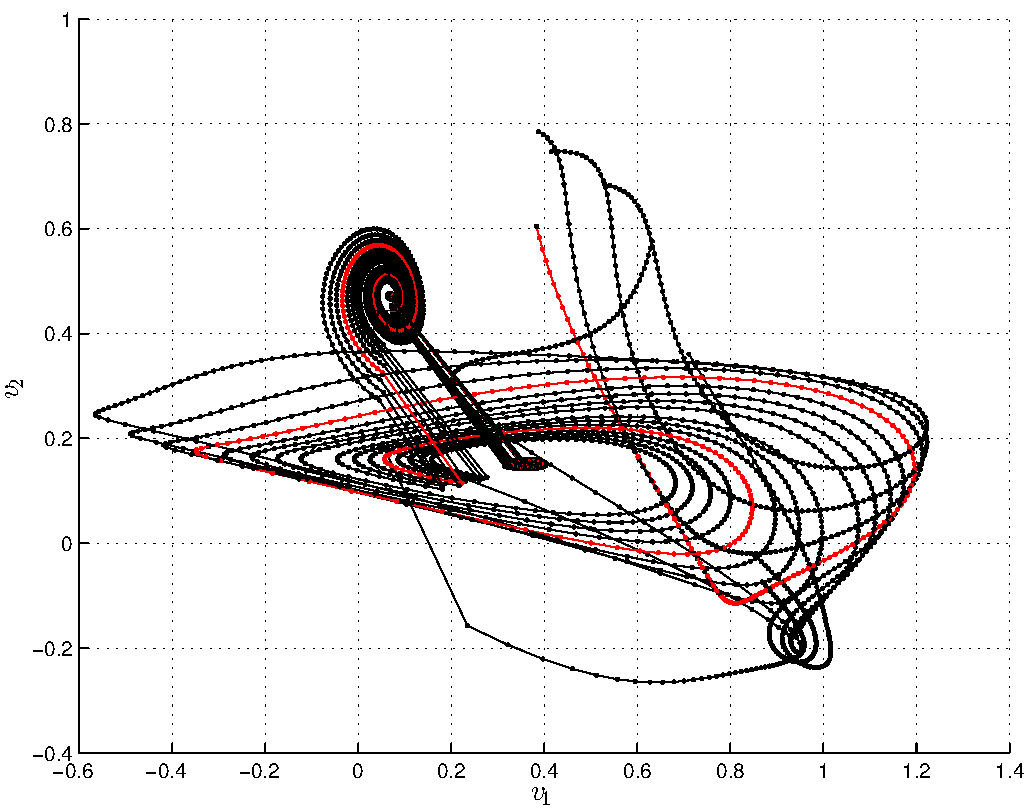
\includegraphics[width=0.45\textwidth, clip=true]{ks22_TW1_manif_inv_mf2_wrapped}~
(b)~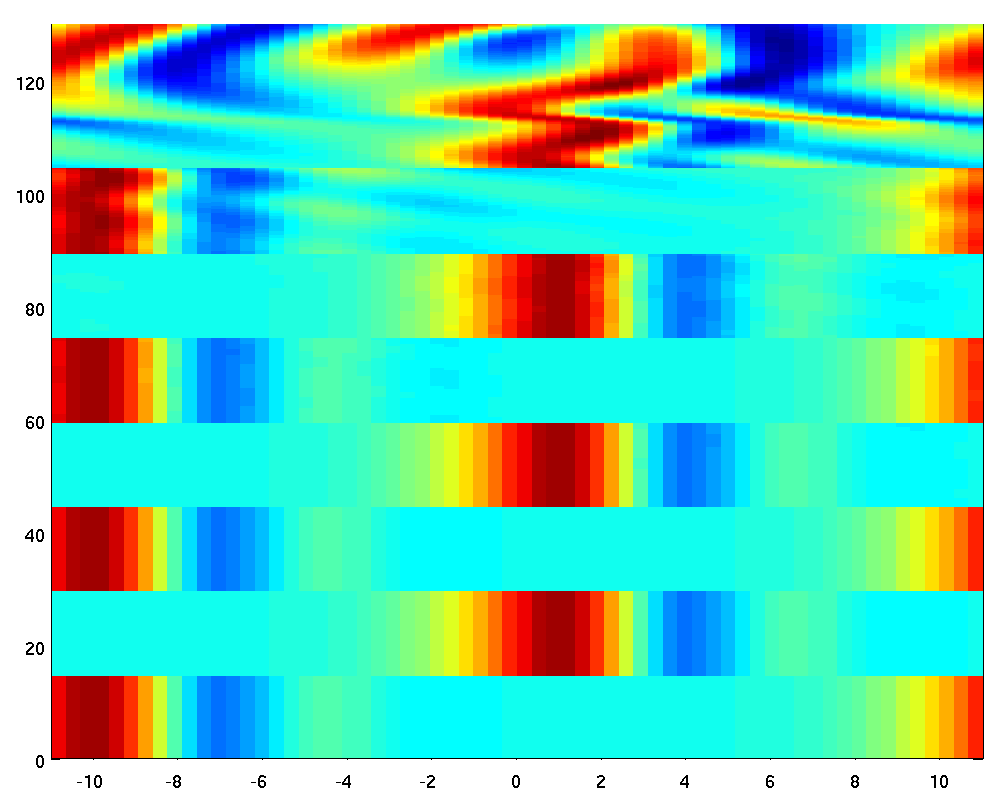
\includegraphics[width=0.20\textwidth, height=0.6\textwidth, clip=true]{ks22_TW1_traj_red_inv_mf2_wrapped}
\end{center}
\caption{
(a) Unstable manifold of \reqv\ \REQV{}{1}, on the slice defined by $c_2=0$,
without the use of Itoh's algorithm for phase unwrapping. (b)
Colormap of $u(x,t)$ for the trajectory shown in
red in panel (a).
The coordinate axes $v_1$, $v_2$ are constructed from vectors Re\,$\jEigvec[1]$,
and Im\,$\jEigvec[1]$ by Gram-Schmidt
orthogonalization.
       }
\label{f:KS22TW1_manif_mf2_wrapped}
\end{figure}

A similar example in the two mode system in the $y_2=0$ slice is plotted in \reffig{f:2modes_unwrapping}.
Note that it is clear that discontinuities occur away from the chart border at $y_1=0$.

\begin{figure}
\begin{center}
(a)~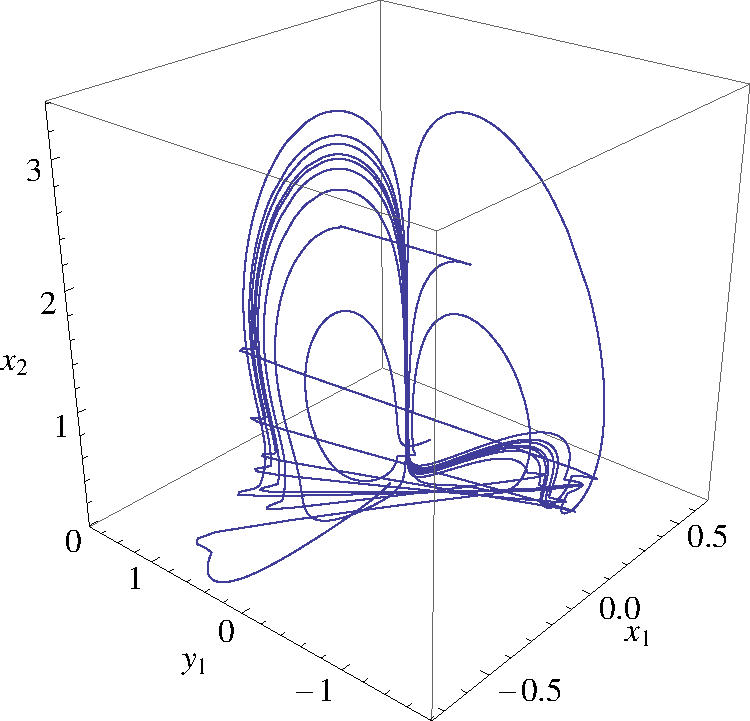
\includegraphics[width=0.45\textwidth, clip=true]{twomodes_mf2_wrapped}~
(b)~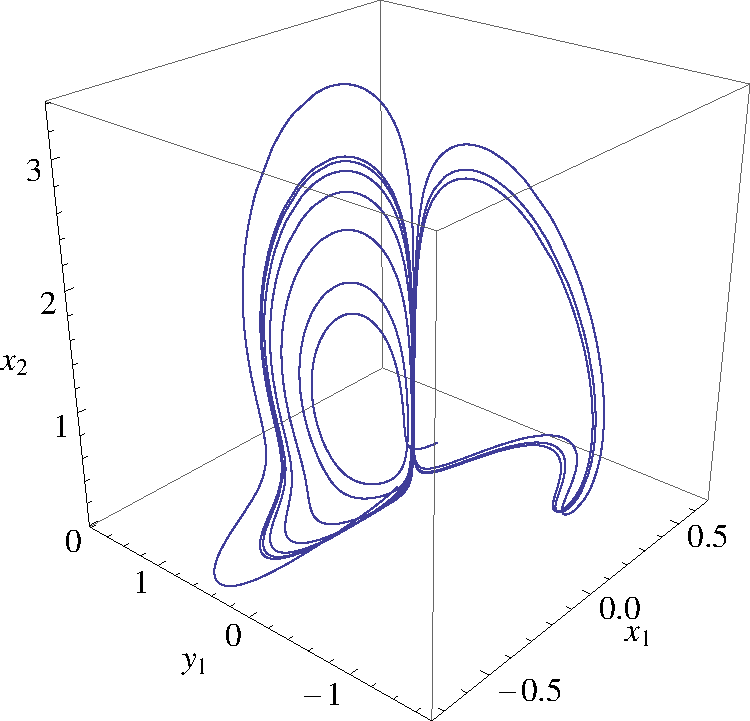
\includegraphics[width=0.45\textwidth, clip=true]{twomodes_mf2_unwrapped}
\end{center}
\caption{
(a) 2 modes system attractor on $y_2=0$ slice using (a) wrapped and (b) unwrapped phase (by Itoh's algorithm).
\BBedit{Burak: These phase jumps are most probably due to the double-valuedness
of the intersections for the second mode slice and will probably go away if
you define the second-mode slice $\sspRed_n = e^{-i n \phi_2} \sspRed_n$
for the complex modes. In this case, this phase-unwrapping is rather scary
because those jumps are actual jumps. As you can see that after phase unwrapping
some parts of the trajectories on the RHS are mirrored onto the LHS, and
the ones for which the transition is smooth are stayed on the RHS.}
\ESedit{Evangelos: Jumps occur whenever $\phi_2$ changes by $2\pi$, for example going through
the 3rd quadrant ($\phi_2=-\pi$) to the 2nd quadrant ($\phi_2=\pi$).
Moving frame angle is $\phi/2$ and therefore changes by $\pi$. This is why you
see jumps in First mode plane, where everything is multiplied by $\phi/2$.
This is purely logistic issue, and has nothing to
do with multivaluedness of slice crossings. The left and right sides of this
attractor should be finally identified by a descrete symmetry reduction, so
I do not see anything scary.}
}
\label{f:2modes_unwrapping}
\end{figure}

\item[2014-05-04 Evangelos] I do not see any problem with uniqueness of the
{\sFslice}, or any other Fourier mode slice, so I will explain
here what I am doing, so that you may correct me if I am wrong. For $k$-mode
slice there is one unique angle defined by
\beq
   \overline{c}_k = b_k\,\sin k\,\theta + c_k\,\cos k\,\theta  = 0\,
   \label{eq:SO2norm}
\eeq
or
\beq
   \theta=-\frac{1}{k}\tan^{-1}\frac{c_k}{b_k} = - \phi_k/k\,.
   \label{eq:SO2mf}
\eeq
Uniqueness is quaranteed by imposing $b_k\geq0$.

The calculated $\phi_k$ for any $k=1\,,\ldots$ presents $2\pi$ jumps. These have to
be compensated by phase unwrapping before computing $\theta=-\phi_k/k$, or otherwise we would
have jumps in $\theta$ that are not multiples of $2\pi$ and therefore would lead
to jumps in reduced state space. This is what is done in \reffig{f:2modes_unwrapping}
and \reffig{f:KS22TW1_manif_mf2_wrapped}. For $k=1$ it is not required because
jumps in $\theta$ are by $2\pi$.

\item[2014-05-02 Burak] Reducing reflection symmetry of \KS\ system along
with the continuous translations:

We will start by slicing (post-processing). When we fix the first mode phase
for reducing the $\SOn{2}$ symmetry, sliced Fourier modes relates to the original
ones by the rotations $\sspRed_n = e^{-i n \phi_1} \ssp_n$, so we can write
the reduced complex Fourier mode amplitudes as follows:
\beq
   \sspRed_n = e^{i (\phi_n - n \phi_1)} | \ssp_n | \quad
   \mbox{where,}\, \ssp_k = |\ssp_k | e^{i \phi_k}
   \label{e-slicean}
\eeq
Now let's look at how the reflection acts on the Fourier modes:
\beq
 R \ssp_n = - \ssp_n^* = e^{i(\pi - \phi_n)} | \ssp_n |,
 \label{e-sspRan}
\eeq
where we denoted the reflection operator with $R$, after slicing, $R \ssp_n$
becomes:
\bea
   \widehat{(R \ssp )}_n &=& e^{i [(\pi - \phi_n) - n (\pi - \phi_1)]} | \ssp_n | , \continue
   &=& e^{i [(1-n) \pi - (\phi_n - n \phi_1 ) ]} | \ssp_n | \continue
   &=& \left\{ \begin{array} {ll}
      e^{i [ \pi - (\phi_n - n \phi_1 ) ]} | \ssp_n | & \quad \mbox{for even n} \\
      e^{- i (\phi_n - n \phi_1 ) } | \ssp_n | & \quad \mbox{for odd n}
   \label{e-sliceRan}
   \end{array}
   \right. . \eea We obtained \refeq{e-sliceRan} from
\refeq{e-slicean} by simply replacing every $\phi_k $ by $ \pi -
\phi_k$. You can see from \ref{e-sliceRan} that combined effect of
reflecting and slicing is different for even and odd modes due to the
$(n-1) \pi$ factor. For odd modes, reflected phase is simply the
negative of the original phase; and for the even modes, there is an
extra factor $\pi$. It is easy to verify that the real and imaginary
parts of the sliced mode components are related to each other as: \bea
   \hat{x}_n &=& - \widehat{(R x)}_n \, , \quad
   \hat{y}_n = \widehat{(R y)}_n \quad \mbox{for even n,} \continue
   \hat{x}_n &=& \widehat{(R x)}_n \, , \quad
   \hat{y}_n = - \widehat{(R y)}_n \quad \mbox{for odd n.}
   \label{e-Rslicerels}
\eea
Where we used the real valued notation $a_n = x_n + i y_n$. I know that the
notation looks confusing, sorry about this, but I could not find a simpler one,
I could have defined a ``slicing'' operator in the beginning. Our final task
is to find a transformation that maps the reduced statespace points related
to each other by the relations \refeq{e-Rslicerels} to the same set of points.
I tried two alternatives \BBedit{(FALSCH: See my entry on [2014-08-08 Burak])}:
\bea
   \tilde{x}_n &=& | \hat{x}_n | \quad \mbox{for even n} \continue
   \tilde{y}_n &=& | \hat{y}_n | \quad \mbox{for odd n} \, , \label{e-tildeabs}
\eea
and
\bea
   \tilde{x}_n &=& (\hat{x}_n)^2 \quad \mbox{for even n} \continue
   \tilde{y}_n &=& (\hat{y}_n)^2 \quad \mbox{for odd n} \, . \label{e-tildesqr}
\eea
Both \refeq{e-tildeabs} and \refeq{e-tildesqr} performs the task that we
need. Transformation \refeq{e-tildeabs} preserves the original units of
the mode components however, its derivative is discontinuous, whereas the
transformation \refeq{e-tildesqr} is smooth but it messes up the dimensionality.
We will see the advantages and disadvantages of the transformations \refeq{e-tildeabs}
and \refeq{e-tildesqr} against each other after more trials, nevertheless,
when we apply one of them, we obtain a representation where both discrete
and continuous symmetries of the \KSe\ are quotiened.

As an example, I applied the transformation \refeq{e-tildesqr} (\ref{e-tildeabs}
also leads to a similar looking result) to the trajectory of a pre-periodic
orbit ($T=35.1698$) after slicing. \refFig{f-BBKS-ppored} shows original
trajectory, sliced and reflection-reduced trajectory in the configuration
space. You can easily see that the pre-periodic orbit closes onto itself
after two periods in the full \statesp\ and in the \slicePlane. When
we reduce the reflections, it closes after one period.

\begin{figure}
\begin{center}
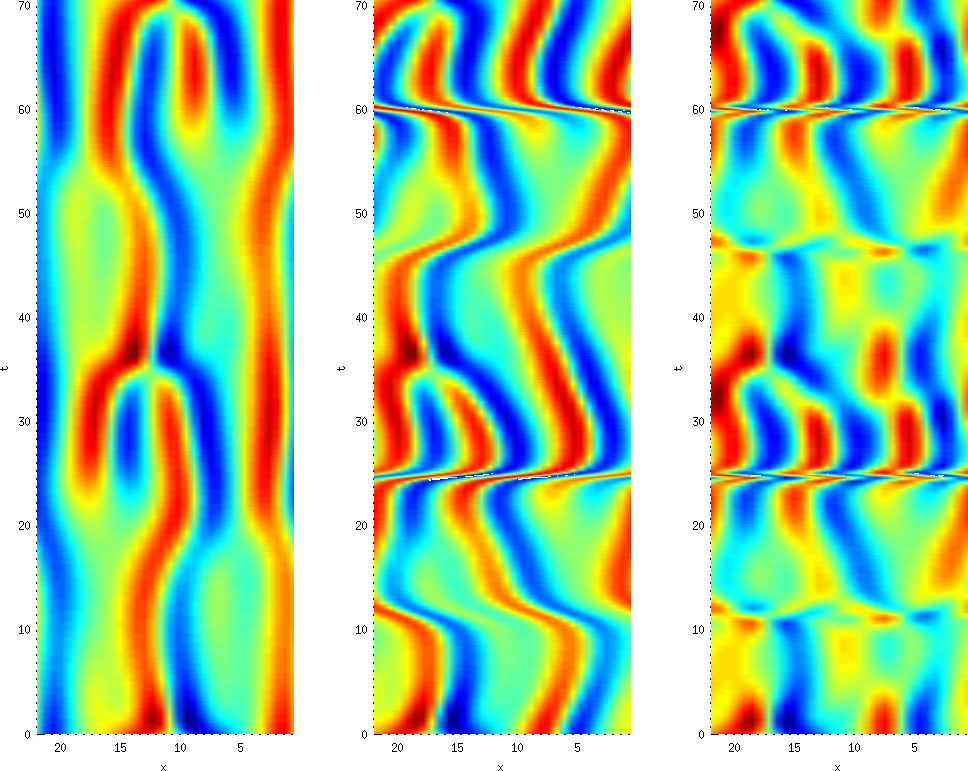
\includegraphics[width=0.90\textwidth, clip=true]{BBKS-ppored}
\end{center}
\caption{Left: Two periods of $PPO_{35.17}$ in full \statesp\ .
Middle: Two periods of $PPO_{35.17}$ after slicing.
Right: Two periods of $PPO_{35.17}$ after reducing reflections by \refeq{e-tildesqr}.}
\label{f-BBKS-ppored}
\end{figure}

\item[2014-05-06 Predrag]
For comparison with \reffig{f-BBKS-ppored} I reproduce here Xiong Ding's
\reffig{fig:ppo2_states_reduced}, 2014-02-25  in
\texttt{siminos/lyapunov} blog. The pre-periodic orbit \cycle{ppo2} is
the 2nd one in Ruslan's database, I have not checked what $\period{ppo2}
=??$ is.
Correct me if I am wrong:

Upon quotienting with \Dn{1}, a pre-periodic orbit \cycle{ppo} of prime period
$\period{ppo}$ becomes a \rpo\ of period $\period{ppo}$ in the \Dn{1}
fundamental domain. Upon subsequent
\SOn{2} reduction,
this \rpo\ becomes a \po\ in the \slicePlane. If one reduces
\SOn{2}\ first, in the slice this becomes a single \po\ of period
$2\,\period{ppo}$, self-dual under \Dn{1} reflection. Under the full
$\On{2}$ reduction the orbit becomes a single \po\ in
the fundamental domain. In the antisymmetric
flow-invariant subspace, one only has \po s and \eqva, all (by
construction) self-dual under \Dn{1} reflection. For each \po\ \SOn{2} than
traces out a torus of symmetry-equivalent \po\ solutions.

\begin{figure}[h]
  \centering
  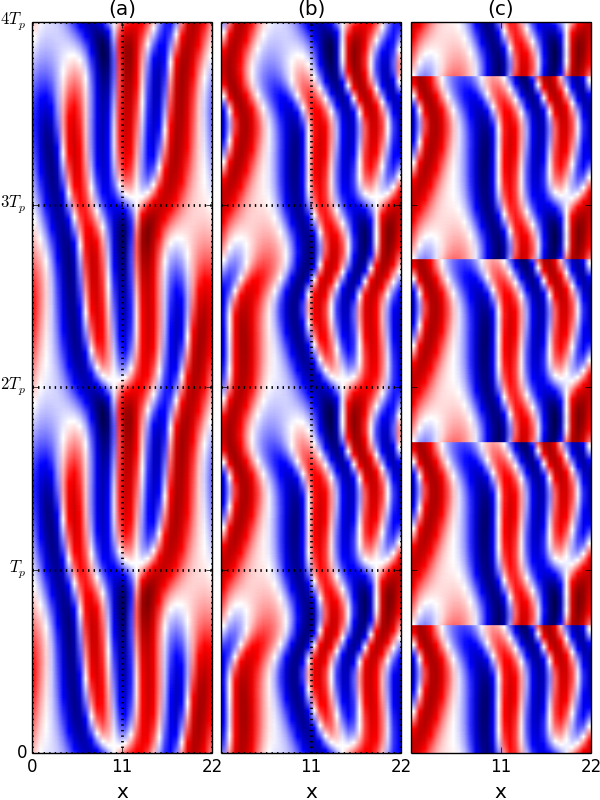
\includegraphics[width=0.7\textwidth]{../xiong/figures/ppo2_state}
  \caption{
Pre-periodic orbit \cycle{ppo2} of prime period  $\period{ppo2} =??$
in configuration space
(a) without symmetry reducing reduction;
(b) after the first Fourier mode \SOn{2} slicing the orbit
closes after two periods;
(c) after \On{2} symmetry reduction the orbit closes after one
period.
    }
  \label{fig:ppo2_states_reduced}
\end{figure}


\item[2014-05-04 Evangelos to Burak] \refeq{e-Rslicerels} is Eqs. (22a)-(22b)
in siminos/ksReduced.tex for $m=1$, so we agree on that! Back then, I also
used \refeq{e-tildeabs} to reduce reflections, until Ruslan stopped me
by pointing out that I was over-reducing, \ie, that one cannot take absolute
values in all Fourier modes. I think he was correct but I do not remember the
exact argument and I cannot find it in the blog. I think you might want to exploit
\refeq{e-Rslicerels} by a fundamental domain type construction.

I would expect that in \reffig{f-BBKS-ppored}
the right panel would look like a reflected version of the
middle panel, but I am afraid that taking squares in \refeq{e-tildesqr}
distorts the patern.
Would it be possible to also plot in \reffig{f-BBKS-ppored},
the result of applying \refeq{e-tildeabs}?

\item[2014-05-05 Burak] It was really hard to tell the difference between
between the outputs of \refeq{e-tildesqr} and \refeq{e-tildeabs} on configuration
space figures by eye, that's why I plotted only the squared version, but
here it is: \reffig{f-BBKS-pporedabs}. You can actually see that the amplitudes
are smaller in the absolute valued version and the turns are sharper. Or
they look to me that way because I know they are :).

The point of \refeq{e-sliceRan} and \refeq{e-Rslicerels} are to identify
the points, within the slice, that are dynamically equivalent due to the
reflection symmetry of the original PDE, and, \refeq{e-tildeabs} and \refeq{e-tildesqr}
are two transformations that simply map these dynamically equivalent points
to a single point. So in this sense, I don't think this is over-reducing,
I think this is what we should do when we have non-commuting symmetries.
I might as well be missing a subtlety in the process, but I can't see it
right now.

The reason why the right panel of \reffig{f-BBKS-ppored} and \reffig{f-BBKS-pporedabs}
don't look like the reflection of the middle panel is because reflections
in the full \statesp\ \refeq{e-sspRan} are not reflections in the \slice ,
they are something else that I cannot assign a geometrical meaning to, but
they are given by \refeq{e-sliceRan}.

\begin{figure}
\begin{center}
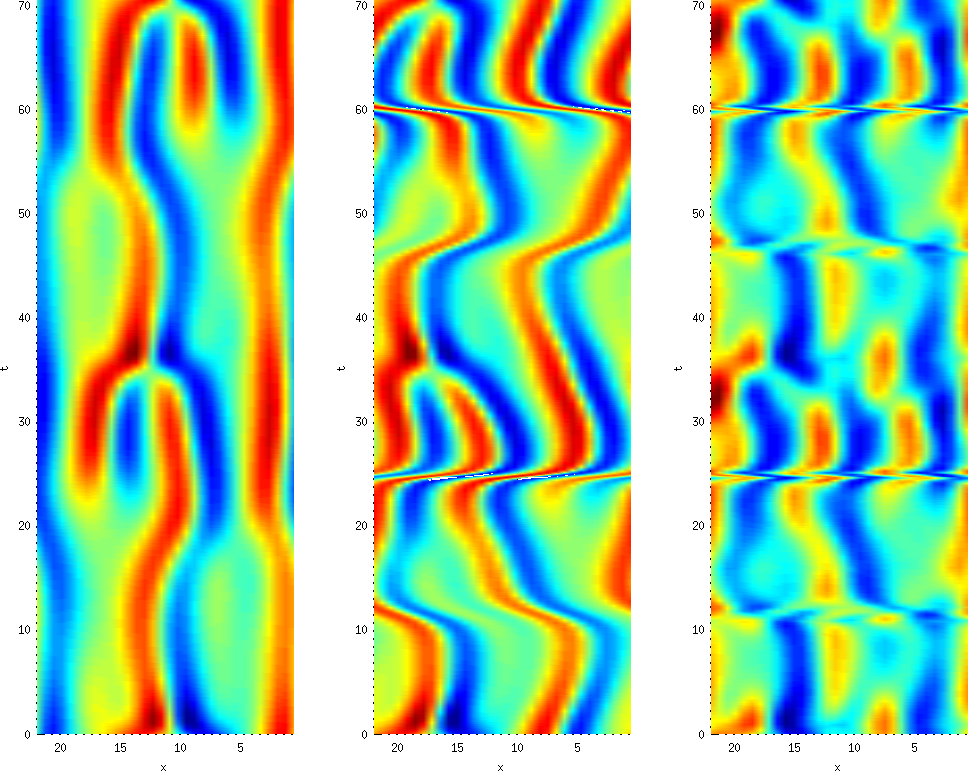
\includegraphics[width=0.90\textwidth, clip=true]{BBKS-pporedabs}
\end{center}
\caption{Left: Two periods of $PPO_{35.17}$ in full \statesp\ .
Middle: Two periods of $PPO_{35.17}$ after slicing.
Right: Two periods of $PPO_{35.17}$ after reducing reflections by \refeq{e-tildeabs}.}
\label{f-BBKS-pporedabs}
\end{figure}

\item[2014-05-03 Burak] Yesterday, I showed that we can reduce the reflection
symmetry by post-processing the sliced evolution. We can get rid off the
$\pi$ jumps due to the border-visits while computing the unstable manifold
of the $EQ_2$ of \KS\ by simply multiplying all the in-\slice\ phases by
2. I'll demonstrate this later, for now, I'm just taking a note here.

\begin{figure}
\begin{center}
(a)~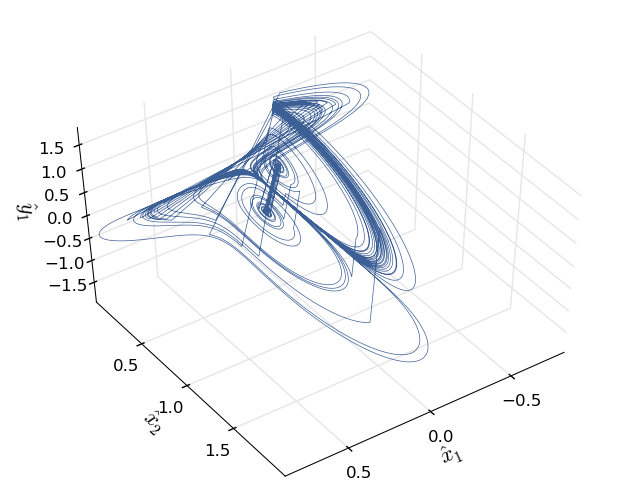
\includegraphics[width=0.45\textwidth, clip=true]{2ndmodeslice}~
(b)~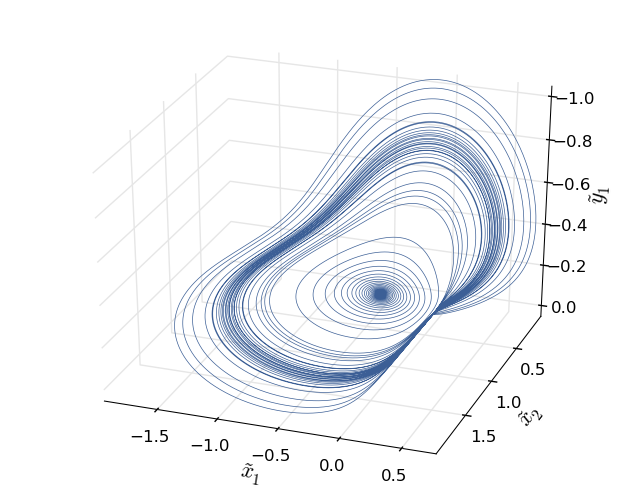
\includegraphics[width=0.45\textwidth, clip=true]{2ndmodeslicephasedoubled}
\end{center}
\caption{(a) \twoMode\ system sliced by fixing the 2nd mode phase, you
can see the $\pi$ jumps in the phase of the first mode due to the wrapped
slicing phase (see the discussion in [2014-05-05 Evangelos and Burak]).
(b) After slicing by fixing the 2nd mode phase, I got rid off the $\pi$
jumps in the phase of the 1st mode by simply multiplying it by 2. }
\label{f-2ndmodeslice}
\end{figure}

\item[2014-05-05 Burak] I was wrong about my  ``non-uniqueness''  guess
in \reffig{f:2modes_unwrapping} caption, jumps are actual border-visit
jumps and I think this is a good demonstration of it. I tried what I suggested
in my [2014-05-03 Burak] entry, and the result is \reffig{f-2ndmodeslice},
I think nice. What I did in \reffig{f-2ndmodeslice} (b) is, after slicing,
I just multiplied the phase of the first mode by 2, so $\pi$ jumps became
$2 \pi$ and hence, invisible. I think this little trick will also help us
with the unstable manifold of $EQ_2$ in \KS .

\item[2014-05-05 Evangelos] \reffig{f-2ndmodeslice} is interesting because it
achieves two goals with one operation: it removes $\pi$ jumps because of
wrapped phase (not border visits) and reduces discrete symmetry of the attractor
by the same trick we applied for Lorenz attractor (see Chaosbook).

However, you have to note that $\pi$ jumps are not close to the chart border
$x_2=y_2=0$ (please label your axes)
and have nothing to do with crossing it. They appear because the value of
arctan in all programs is restricted to the interval $(0,2\pi)$ or $(-\pi,\pi)$,
while in reality it should be allowed to vary outside this interval.
(I make a note to upload a figure to demonstrate this.)
Itoh's algorithm solves this in a consistent manner. I am a bit afraid
that if we try to apply the angle-doubling trick for KSe with, e.g. second mode slice,
we will create some logistic nightmare with the higher modes. But you can try and
see. In principle I think one should first unwrap the phase, then go to reduced
space, identify discrete symmetries and quotient them (by a trick such as angle
doubling or whatever is appropriate for each case).

Regarding unstable manifold of KSe \EQV{2}, there the difficulty is due to genuine
border crossings (I make a note to upload a figure to also demonstrate this)
and occurs whatever Fourier mode we use for the slice. Note that in that case,
instead of modifying Itoh's algorithm to explicitly remove $\pi$ jumps, I multiply
the time series of $\theta$ with 2, apply the algorithm and then divide by 2.
I think that if you simply multiply the angle by 2 in this case, you will have
continuity, but will also rotate your slice. But you can try.

\item[2014-05-05 Burak]  I was careless in interpreting \reffig{f-2ndmodeslice},
as Evangelos said, jumps are not due to the border visits, but to the discontinuity
of the $\arctan$, which was what I tried to mean in my comment on \reffig{f:2modes_unwrapping},
but the situation was also not clear to me at that time. Anyways, its true
that the wrapped $\arctan(y_2 / x_2)$ has $2 \pi$ jumps, and when we use
it to slice, $2 \pi$ jumps becomes $\pi$ on the first mode and we get
\reffig{f-2ndmodeslice}(a). Multiplication of the 1st mode phase by $2$
clears this. This simple idea can be extended to higher mode slices for \KS ,
for example, if we try slicing \KS\ by fixing the phase of, say $6th$ mode,
we are going to have discontinouity in the phases of first five modes, which
we can easily fix by multiplying the phase of each $n<6$ mode by $n$, without
losing any information. This, I think, is something to keep in mind and
experiment on.

\item[2014-05-09 Evangelos] I tried to check Burak's prescription of doubling the angle
for KS. See \reffig{f:KS22TW1_manif_mf2_double}(b) for the result when plotting
\REQV{}{1} unstable manifold in second mode slice. I think the problem is that implicit in
Burak's prescription there is the assumption that in reduced space there is a descrete
symmetry of rotations by $\pi$. This is true for the \twoMode\ system, but will not be
true in general.

Eventhough this trick works for the \twoMode, I would suggest that also in that
paper we should illustrate this as a two step procedure. First use Itoh's algorithm
(you can find my implementation in siminos/matlab/ruslan/itoh.m) to obtain a two-ear
attractor. Then in a seperate section on residual discrete symmetry reduction
apply your (and chaosbook.org) trick of doubling the angle.

There also seems to be residual descrete symmetry for the first mode slice in the \twoMode\
system. You may also want to think how to get rid of that. I think you might still be
able to play the angle doubling game here.

It would be interesting to try to see explicitly this discrete symmetry in \twoMode\
equations on the slice.

\begin{figure}
\begin{center}
(a)~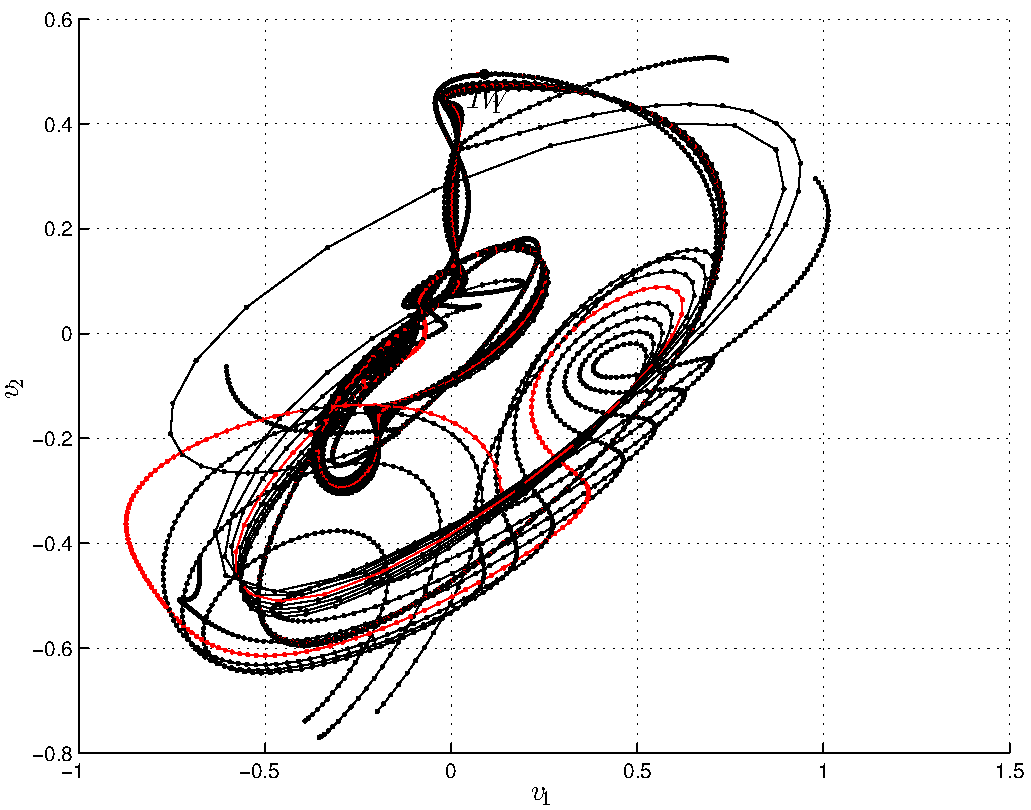
\includegraphics[width=0.45\textwidth, clip=true]{ks22_TW1_manif_inv_mf2_double}~
 (b)~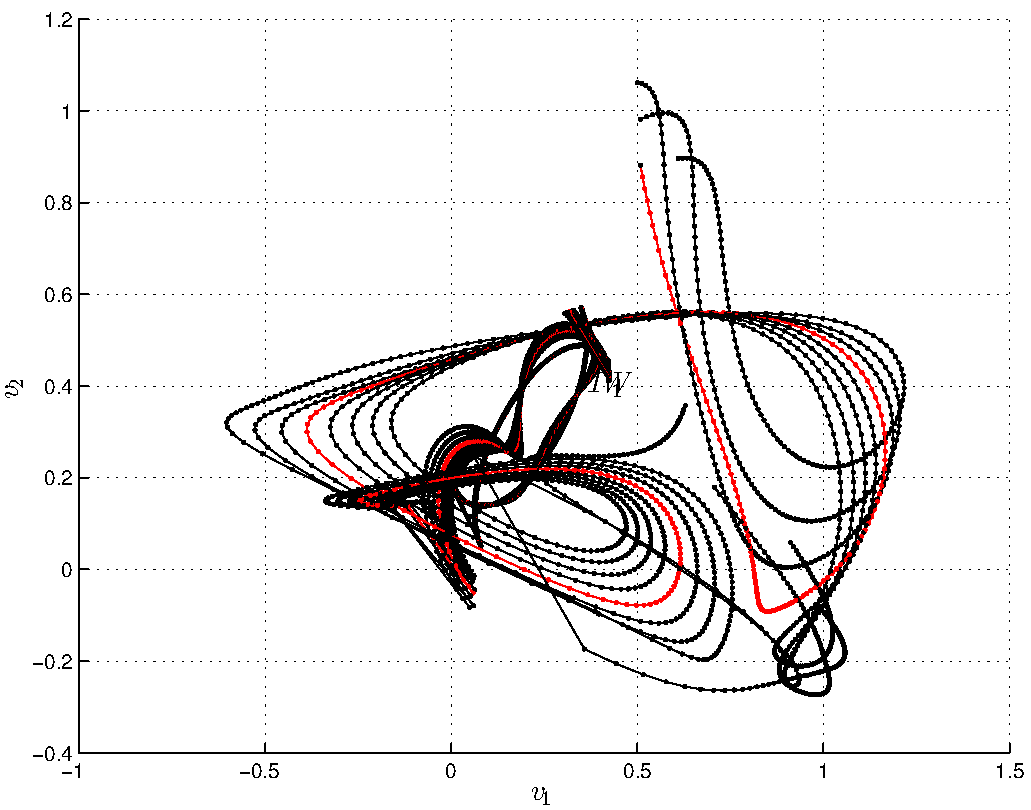
\includegraphics[width=0.45\textwidth, clip=true]{ks22_TW1_manif_inv_mf2_double_1mode}
\end{center}
\caption{
(a) Unstable manifold of \reqv\ \REQV{}{1}, on the slice defined by $c_2=0$,
after doubling the moving frame angle,
(b) using Burak's prescription of doubling the \emph{first mode} angle.
The coordinate axes $v_1$, $v_2$ are constructed from vectors Re\,$\jEigvec[1]$,
and Im\,$\jEigvec[1]$ by Gram-Schmidt
orthogonalization.
       }
\label{f:KS22TW1_manif_mf2_double}
\end{figure}

\item[2014-05-09 Burak to Evangelos] How do you compute eigenvectors? Are they linear stability
eigenvectors within the second mode slice?

\item[2014-05-09 Evangelos to Burak]
See \refref{SCD07} for computation of stability matrix of relative equilibria that I use here.
We could discuss if this is correct or not, but I have to note that this cannot cause any
problem in \reffig{f:KS22TW1_manif_mf2_double}, since everything is done by postprocessing
trajectories as in \reffig{f:KS22TW1_manif_mf}.

\item[2014-05-09 Burak to Evangelos] Also, can you apply the same procedure to the
unstable manifold of $EQ_2$? Since the second mode subspace is of dynamical interest there,
I was expecting this treatment to be helpful in visualizing that.

\item[2014-05-09 Evangelos to Burak] See comment [2014-05-05 Evangelos] above.

\item[2014-05-09 Burak to Evangelos] I, by the way, wrote it down in the 2modes paper (see git repo).
Also, are you doubling all the phases? or only the first mode phase?
Doubling each phase makes trajectories very complicated since everything rotates twice as much, however,
if you just double the $1st$ mode phase in the second mode slice, you'll get rid off the $\pi$ jumps,
and that's it. That's what I wrote to the current draft of the \twoMode\ paper.

\item[2014-05-09 Evangelos to Burak] See \reffig{f:KS22TW1_manif_mf2_double}(b) for the result of
doubling only the phase of first mode angle. You still have discontinuities because you get, e.g.,
$3\pi$ jumps for third Fourier mode, etc.

Moreover, the reason we like slicing in the first place is that it corresponds to a simple geometric operation
of rotating state space points. If you only double first mode angle, then this is not equivalent to
a rotation and I have trouble to understand what it does.

I've seen the text in \twoMode\ paper and I think we have to present it explicitly,
as a two step procedure. We also need to understand if the discrete symmetry in reduced space is
inherent in the \twoMode\ model or is induced by slicing.

In any case, there is no reason to avoid unwrapping $2\pi$ jumps. I think it's a standard thing to do
in e.g. interferometry (that's how I came to know about it) and it removes all ``trivial'' discontinuities,
i.e. caused by atan or atan2. The only question is why haven't we done it before?

\item[2014-05-09 Burak] Oh, Ok. I got it, then may be doubling phases of
the odd modes only? Please don't waste your time if you think this is an
unnecessary experiment. I'm working on \twoMode\ \rpo s right now, once
that I finish producing results for that paper, I'll start again with the
\KS .

\item[2014-06-26 Evangelos] I have run into trouble with reduction of a
\rpo\ that comes close to \EQV{2}, see
\reffig{f:ks22_E2_manifold_mf1_rpo4764}. The \rpo\ closes only after the
second period, and I think that this has to do with the fact that we do
not reduce reflections. For $m=2$ slice, it takes 4 periods before the
\rpo\ returns to initial point, so there must be an additional discrete
symmetry introduced by slicing, as in the case of Porter-Knobloch flow.
Also, I see some kinks, which are probably caused by close passages to
the {\sliceBord}. Here I use the method of moving frames, but it would be
better to use intergration in rescalled time. Burak, could you please
tell me how to use your code (preferably in matlab)? Also, did you
implement higher slices in your code? It should be a very easy change.

\begin{figure}
\begin{center}
(a)~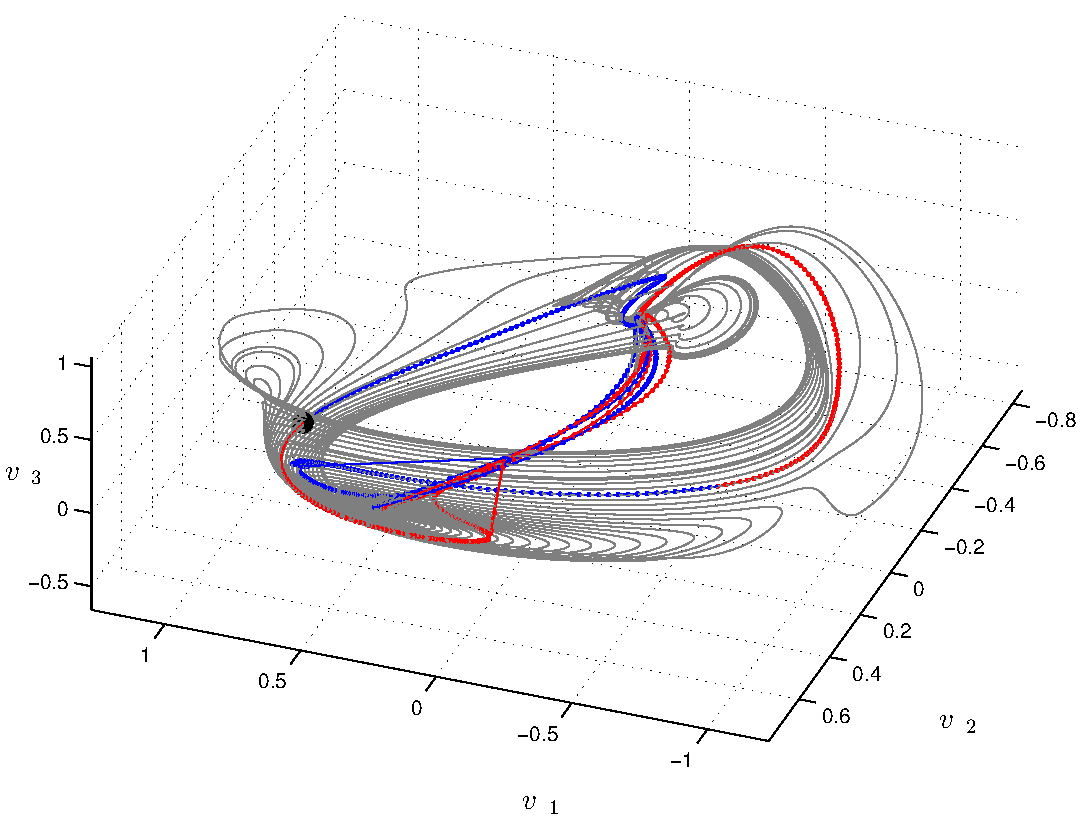
\includegraphics[width=0.45\textwidth, clip=true]{ks22_E2_manifold_mf1_rpo4764}~
(b)~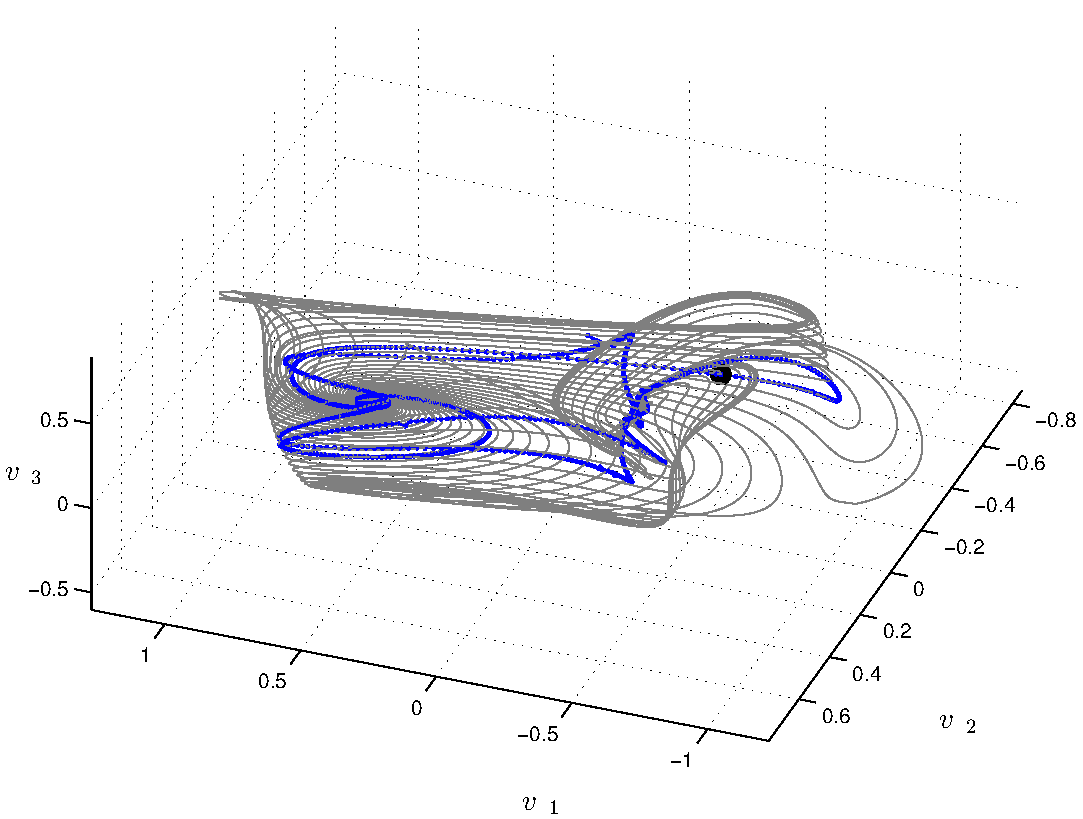
\includegraphics[width=0.45\textwidth, clip=true]{ks22_E2_manifold_mf2_rpo4764}~
\end{center}
\caption{
Unstable manifold of \EQV{2} and \rpo\ with $T=47.64$ and $s=5.7$,
on the slice defined by (a) $c_1=0$, (b) $c_2=0$ (using $pi$-unwrapped phase).
In (a), two periods are shown;
the first period is shown in blue, the second in red, and the initial condition is shown as a black dot.
In (b) four periods are shown (in blue).
The coordinate axes $v_1$, $v_2$ are constructed from vectors Re\,$\jEigvec[1]$,
and Im\,$\jEigvec[1]$ by Gram-Schmidt
orthogonalization.
       }
\label{f:ks22_E2_manifold_mf1_rpo4764}
\end{figure}

\item[2014-06-26 Burak] My slice-time integrator for the Kuramoto-Sivashinsky is in

\texttt{siminos/ksConnected/ksETDRK4red.m}, and in case you need it, stability matrix
in the first-mode slice is in the same folder, named \texttt{gradVred.m}. They are
tested in both Matlab and Octave they should be fine. You can check
\texttt{siminos/ksConnected/TWmanifold.m} for a an example of use of these m-files.

You should have \texttt{siminos/ksConnected/pars.m} in the same folder to run these
functions, it sets the system size and number of modes.

As for the second mode slice, it's not all obvious to me to how to implement
it, because I had to do a few tricks to make ETDRK4 work for the first-mode slice,
but it should be doable. I'll probably have it ready for you sometime in this
weeekend.

\item[2014-06-27 Evangelos] Thanks a lot! I tried it and it works as advertised.
I created a copy in \texttt{siminos/matlab/ruslan/ksETDRK4red1.m} in which I changed
the input/output arguments, so that 1) you do not need to read parameters from pars.m,
but instead you pass them as arguments, 2) the argument list matches as much as possible
Ruslan's ksfmetd2.m. Burak if you would like to propagate these edits back into your
original file, be careful with the changes in the order of the arguments!
At the end it would be better to only have one version of each routine and
install it somewhere in matlab's path, but I do not know how to do this.

\item[2014-06-27 Evangelos] Using Burak's in-slice time integration the \RPO{47.64} closes after
a single period for $m=1$ slice! See \reffig{f:ks22_E2_manifold_slice1_rpo4764}.
I am probably doing something wrong in postprocessing for moving frame method in \reffig{f:ks22_E2_manifold_mf1_rpo4764}.
In \reffig{f:ks22_E2_manifold_slice1_rpo4764}
I colorcode values with $|\hat{b}_1|<0$ differently, so that we can see that large part of the trajectory
is dominating by the extreme stretching close to the chart border. This is annoying to show like
this in a paper, but for \PoincSec s we should be safe as long as we define them
away from the chart border.

It would be cool if we could think of a coordinate transformation
that shrinks the points close to the chart border.

Code for second mode slice is eagerly awaited :-) If something
interesting happens close to \EQV{2}, then it should be easier to see in
$m=2$ chart.

\item[2014-06-27 Burak] If you are using \SOn{2} formulation, you might want
to check your rotation matrices, because before the slice paper they were
left-handed everywhere. I'm working on the in slice integration of $m=2$.

\item[2014-06-28 Evangelos] Thanks, I will check that.

\begin{figure}
\begin{center}
(a)~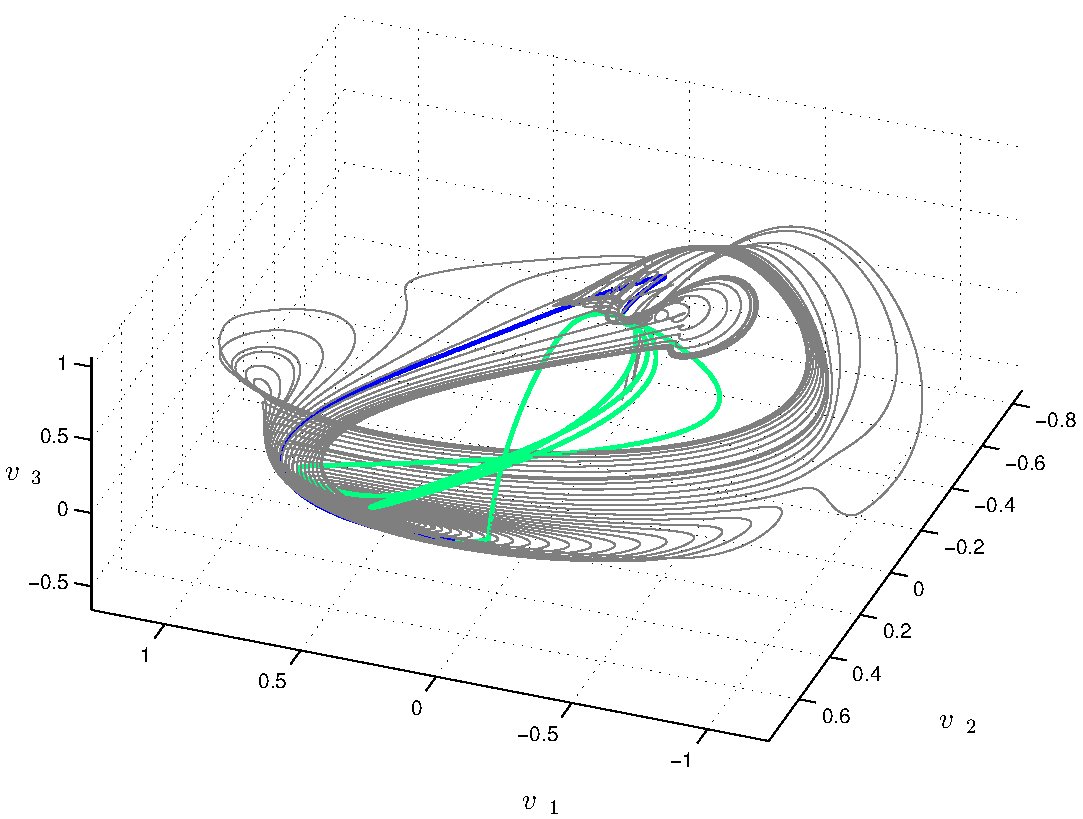
\includegraphics[width=0.45\textwidth, clip=true]{ks22_E2_manifold_slice1_rpo4764}~
(b)~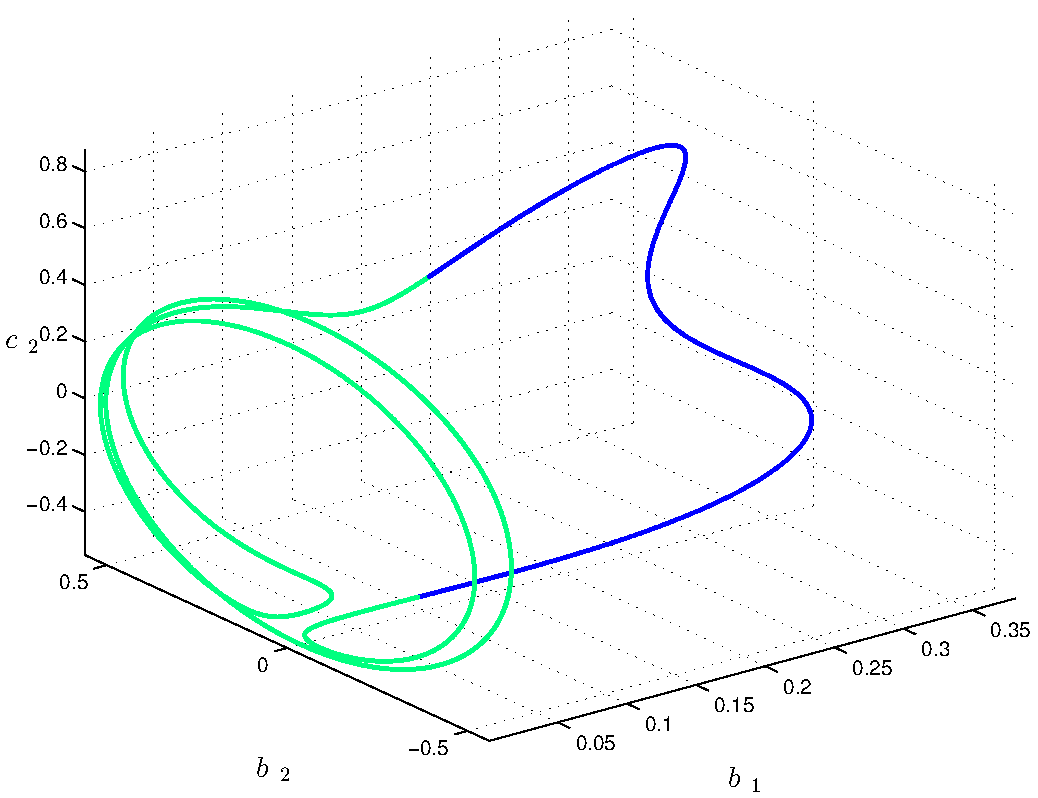
\includegraphics[width=0.45\textwidth, clip=true]{ks22_rpo4764_slice1_fm}~
\end{center}
\caption{
(a) Unstable manifold of \EQV{2} and \rpo\ \RPO{47.64} with $T=47.64$ and $s=5.7$,
on the slice defined by $c_1=0$, using integration on the slice for \RPO{47.64} only
(not for the manifold of \EQV{2}).
A single period of \RPO{47.64} is shown, Blue indicates $|\hat{b}_1|>0.1$, green indicates
 $|\hat{b}_1|<0.1$.
The coordinate axes $v_1$, $v_2$ are constructed from vectors Re\,$\jEigvec[1]$,
and Im\,$\jEigvec[1]$ by Gram-Schmidt
orthogonalization.
(b)  \RPO{47.64} in Fourier mode projection (in slice), colorcoded as above.
       }
\label{f:ks22_E2_manifold_slice1_rpo4764}
\end{figure}

\item[2014-06-29 Evangelos]
I tried a few more different representations, but it is getting too late here.
I will blog tomorrow the figures tomorrow.
% \reffig{f:ks22_E2_manifold_slice1_rpo4764_prob}(a) is the same as
% \reffig{f:ks22_E2_manifold_slice1_rpo4764}(a), but in Fourier mode projection.
% It shows that it

\item[2014-06-29 Evangelos] \reffig{f:ks22_E2_manifold_slice1_rpo4764_prob}(a) is the same as
\reffig{f:ks22_E2_manifold_slice1_rpo4764}(a), but in Fourier mode projection.
Here it becomes obvious that the attempt to bring the unstable manifold of
\EQV{2} to the $\tilde{c}_1=0$, $\tilde{b}_1>0$ slice has met fundamental difficulties.
As a reminder, the unstable manifold of \EQV{2} leaves in a subspace which
under \SOn{2} is rotated uniformly. Therefore, one can try to bring the whole
manifold to the $c_1=0$ slice by a rotation by appropriate angle, or by
anwrapping moving frame angle when jumps of $\pi$ occur. Eventhough in both
cases we get a manifold that has no singularities, the manifold extents to
negative $b_1$. At the same time, \RPO{47.64} integrated on the slice does not
move past the $b_1=0$ border.

One way out of the difficulty, would be to try to relax the $\tilde{b}_1>0$ condition
when slicing. \reffig{f:ks22_E2_manifold_slice1_rpo4764_prob}(a) suggests we would
get trajectories with descrete symmetry and then we would have to reduce that
symmetry. For general orbits, this would probably give us the same results as
integration on the slice. For unstable manifold of \EQV{2}, one could probably
think of an operation that folds back the manifold to the $\tilde{b}_1>0$ half-space.
I think taking absolute value of $\tilde{b}_1$ is sufficient. I will try this next.

Another option is to try our regular slicing also for the unstable manifold of
\EQV{2}, \ie, let the manifold have jumps of $\pm\pi$. This is shown in \reffig{f:ks22_E2_manifold_slice1_rpo4764_prob}(b).
I think these jumps correspond to genuine slice crossings, because the flow is restricted
to a low dimensional subspace. I tried to use Burak's in-slice time integrator to
integrate initial conditions on the unstable manifold of \EQV{2}, in
order to prove myself wrong. It seems that the integrator stagnates, indicating a
genuine slice crossing, but I would have to look in to this more closely.
Burak, would it be possible to include an exit condition in your code,
allowing to return a solution if $b_1$ becomes of the order of machine $\epsilon$?

\item[2014-06-30 Burak] When I tried to compute the unstable manifold of \EQV{2},
I also got stagnating trajectories, so I agree that border crossings happen on
the unstable manfiold of \EQV{2}.

\begin{figure}[ht!]
\begin{center}
(a)~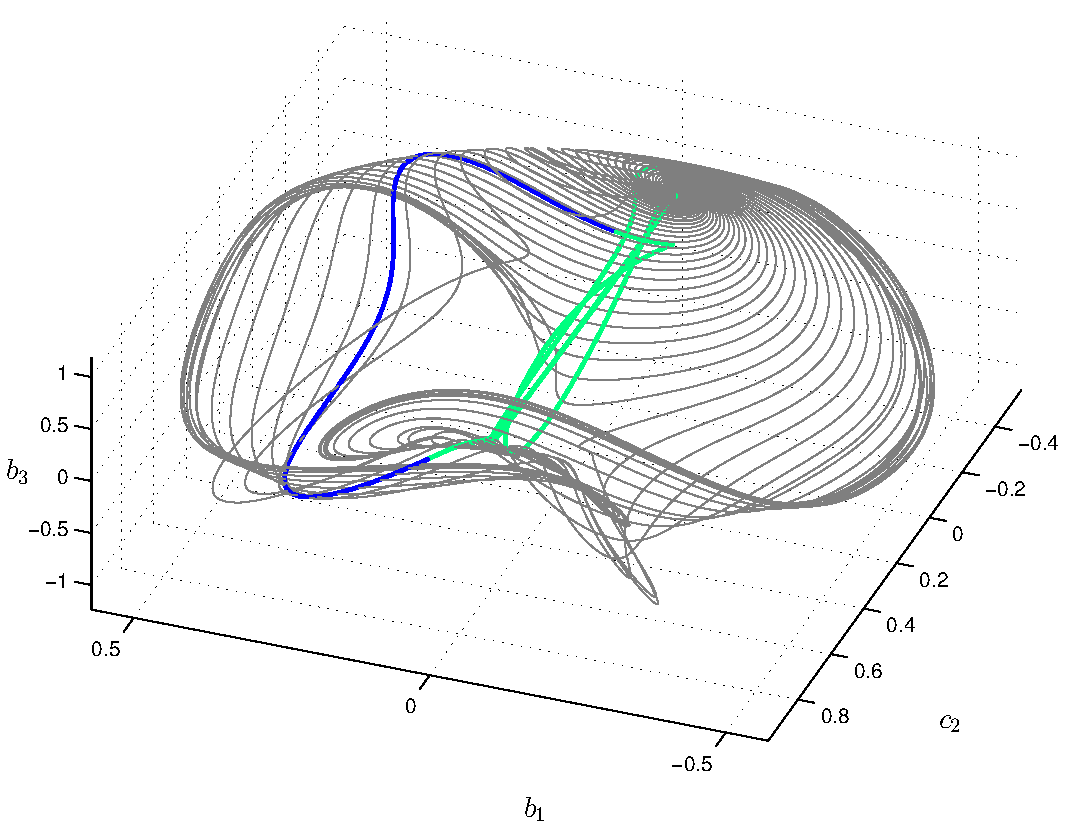
\includegraphics[width=0.45\textwidth, clip=true]{ks22_E2_manifold_mf1_rpo4764_rotated}~
(b)~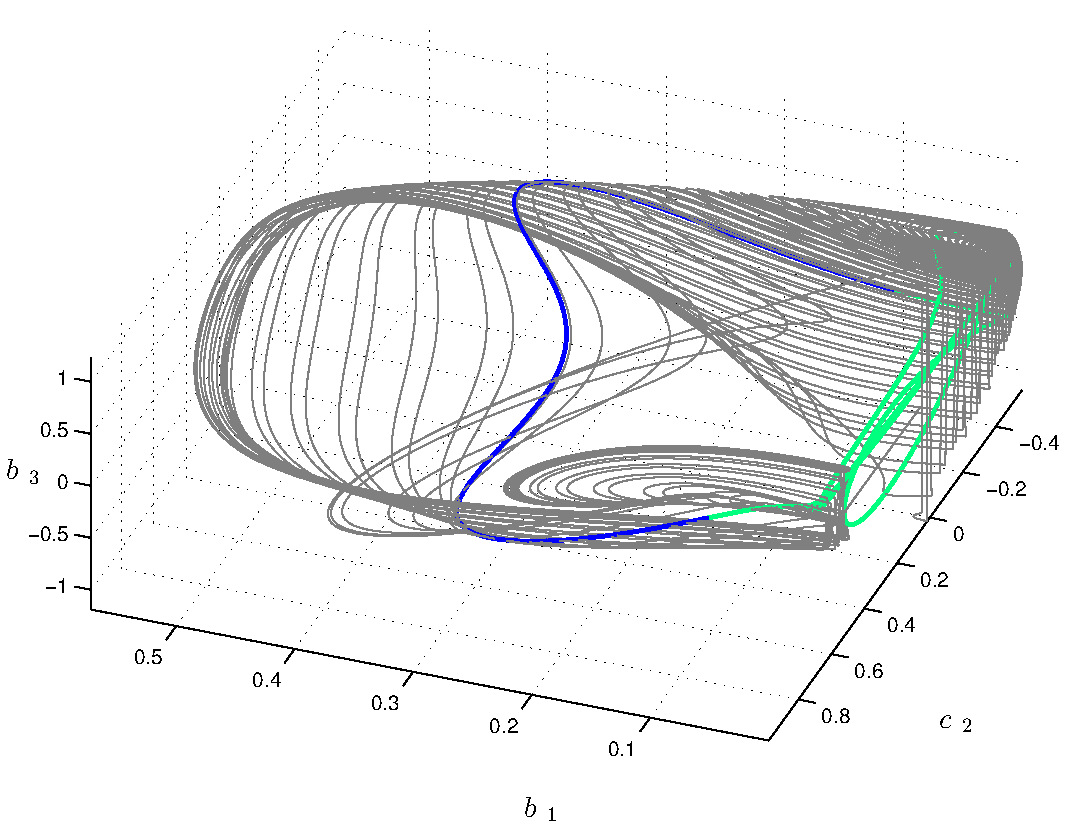
\includegraphics[width=0.45\textwidth, clip=true]{ks22_E2_manifold_mf1_rpo4764_no_itohPi}~
\end{center}
\caption{
Unstable manifold of \EQV{2} and \rpo\ \RPO{47.64} with $T=47.64$ and $s=5.7$,
on the slice defined by $c_1=0$, using integration on the slice for \RPO{47.64} only
(not for the manifold of \EQV{2}), Fourier modes projection.
A single period of \RPO{47.64} is shown, blue indicates $|\hat{b}_1|>0.1$, green indicates
 $|\hat{b}_1|<0.1$.
(a) The initial conditions for the unstable manifold of \EQV{2} have been rotated
to the slice, then integrated in original space.
(b) The unstable manifold of \EQV{2} has been rotated to the slice without
 using the $\pi$-unwrapping trick.
       }
\label{f:ks22_E2_manifold_slice1_rpo4764_prob}
\end{figure}

\item[2014-06-29 Evangelos] Since we know that the stretching close to the chart
border is caused by a $1/\hat{b}_1^2$ factor that appears in all reduced space variables,
see \refref{SiminosThesis}, we may try to obtain a less singular representation by
multiplying the slice variables $\hat{a}_j$ by a factor of $\hat{b}_1^2$. This gives us
a basis of invariant polynomials for free, and eliminates the rapid stretching close
to the origin, see \reffig{f:ks22_E2_manifold_slice1_rpo4764_ip}. Also, there are no
overflow problems that one might have in direct evaluation of high order invariant
polynomials. Here, we only multiply by $\hat{b}_1^2$ which has finite value.

A drawback is that we can now discern less of the dynamics close to \EQV{2}, but maybe
this is just a visualization noisance. I hope that topological information is not
lost. I would expect the cycle symbolic dynamics to be related to number of ``turns''
around \EQV{2}. Using $m=2$ or $m=6$ slice would be more appropriate, so that \EQV{2} is
not on the chart border.
Also, we have to check how \hec\ to \EQV{3} appears in this representation.

In any case, this is just a temporary solution to allow visualization.
I hope we can find a reasonable solution
for the unstable manifold of \EQV{2} within the slicing framework.

\begin{figure}[ht!]
\begin{center}
(a)~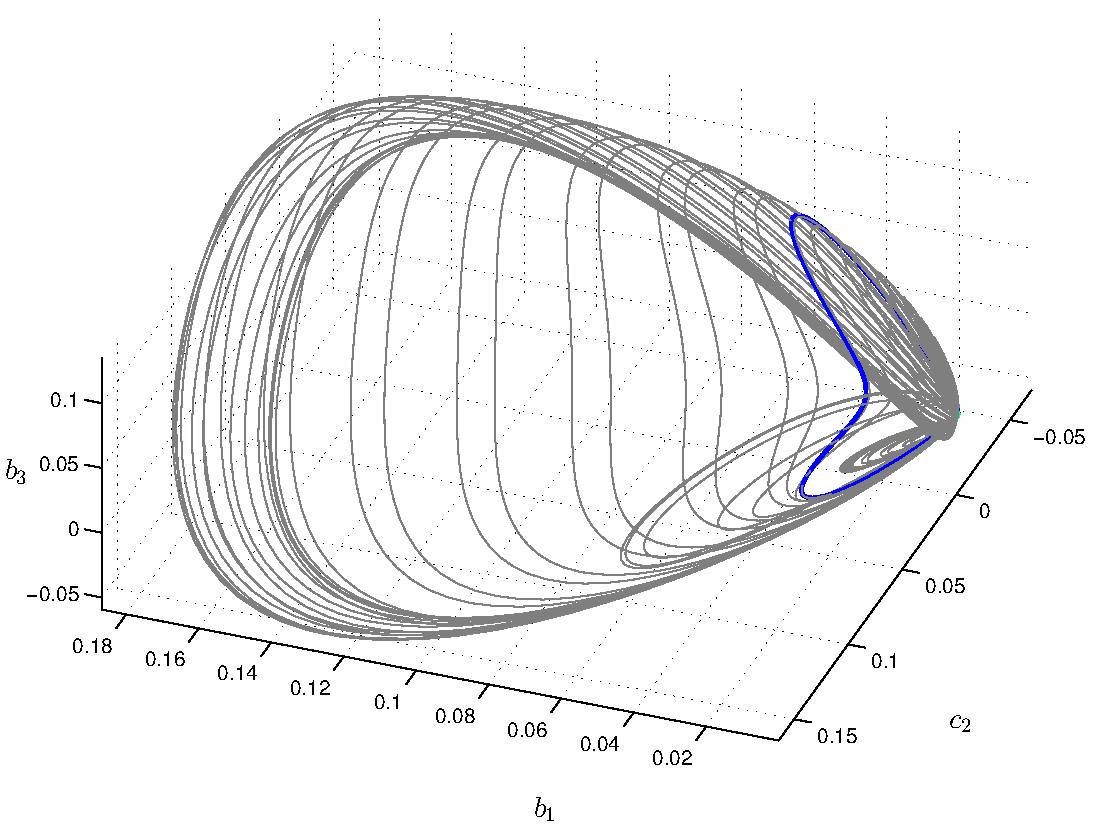
\includegraphics[width=0.45\textwidth, clip=true]{ks22_E2_manifold_fm_ip}~
(b)~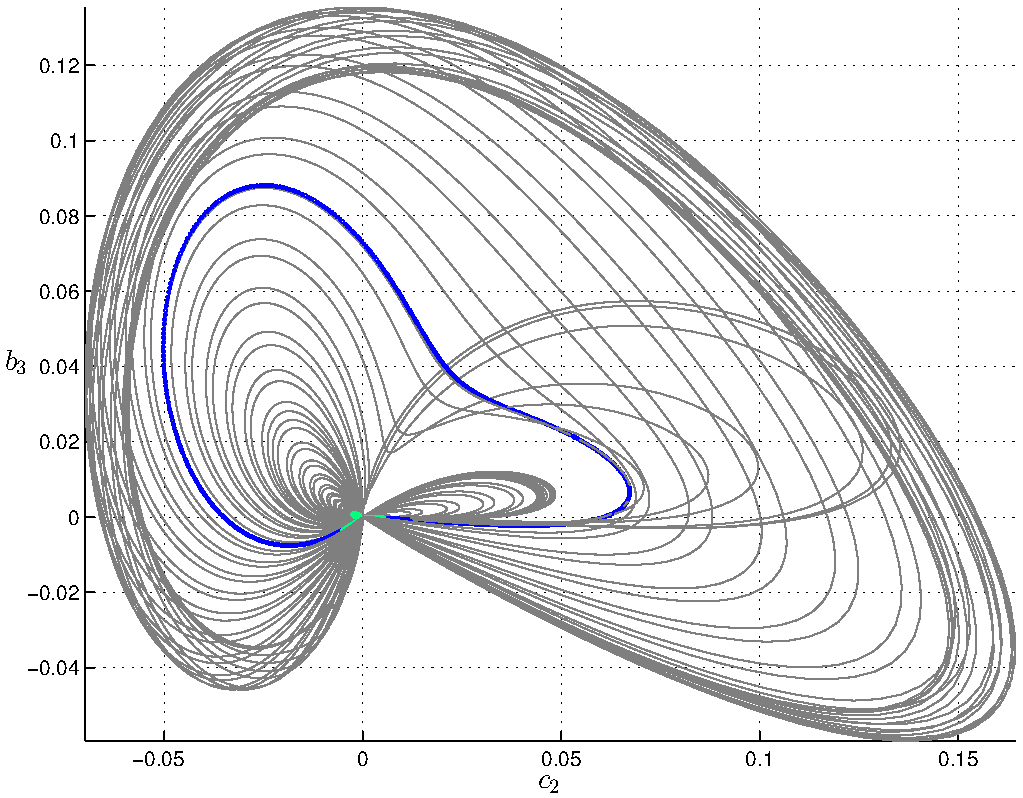
\includegraphics[width=0.45\textwidth, clip=true]{ks22_E2_manifold_fm_ip2}~
\end{center}
\caption{
Unstable manifold of \EQV{2} and \rpo\ \RPO{47.64} with $T=47.64$ and $s=5.7$,
on the slice defined by $c_1=0$, using integration on the slice for \RPO{47.64} only
(not for the manifold of \EQV{2}).
A single period of \RPO{47.64} is shown. Blue indicates $|\hat{b}_1|>0.1$, green indicates
 $|\hat{b}_1|<0.1$.
(a) Same as \reffig{f:ks22_E2_manifold_slice1_rpo4764_prob}(b), but passing to invariant
polynomials by multiplying all variables by  $\hat{b}_1^2$.
(b) Same as in (a), different projection.
       }
\label{f:ks22_E2_manifold_slice1_rpo4764_ip}
\end{figure}

\item[2014-06-30 Burak] I finished in-slice integrator for the 2nd mode slice,
its input/outputs are similar to the previous one and it's here:

\texttt{siminos/ksConnected/ksETDRK4red2.m}

I added an `if' inside the integrator that breaks the loop when it gets to a
stagnation point. I tried to compute unstable manifold of \EQV{2} on the 2nd
mode slice, however, all the trajectories went to the stagnation points after
some time. That code is here:

\texttt{siminos/ksConnected/eq2manifold.m}

\item[2014-08-08 Burak] After a little bit thinking, I figured why
\refeq{e-tildeabs} and \refeq{e-tildesqr}
are over-reducing. Take, for example, the case when only one of the coordinates
flips its sign, say $x_2 \rightarrow -x_2$, this is not a reflection operation,
however \refeq{e-tildeabs} and \refeq{e-tildesqr} are invariant under that operation
so they do much more than reducing reflection symmetry. Since we have seen that a
`fundamental domain' description makes the flow discontinuous, I'm still trying
to find a method of constructing a basis set that is invariant under reflections.

In this perspective, I want to re-describe the problem:
We can represent the reflection operator in the first Fourier mode slice as follows:
\beq
    R = \mathrm{diag} (1, -1, -1, 1, 1, -1, -1, 1, ...)
\eeq
This operator satisfies $R^2 = e$ where $e$ is the identity, and leaves the hyperplane
$(\hat{x}_1, 0, 0, \hat{y}_2, \hat{x}_3, 0, 0, \hat{y}_3, ...)$ invariant. Now the
coordinates that flips the sign under the action of $R$ are:
\beq
 \hat{y}_1, \hat{x}_2, \hat{y}_3, \hat{x}_4, \hat{y}_5, \hat{x}_6, \hat{y}_7, \hat{x}_8, ...
 \label{e-xRefs}
\eeq
and any second order term that we can write using these coordinates is invariant
under reflections. Now my question is:

\emph{Can we find a tractable algorithm of picking
set $S = \{p_1, p_2, p_3, p_4, ...\}$ where  $p_i$ are second order in any two coordinates
in \refeq{e-xRefs}, such that using $S$, we can find all coordinates listed in
\refeq{e-xRefs} upto one minus sign?}

This minus sign ambiguity would correspond to
the choice of the `fundamental domain', however, there must be only one choice of
plus or minus sign. For example, \refeq{e-tildesqr} is combinations of second order
terms, however, there are $n$ undetermined $\pm$ sign in the back-transform, therefore
it is over-reduction.

An obvious answer to this question would be taking all second order terms containing
coordinates in \refeq{e-xRefs}. However, of course, we would get way too many
polynomials this way (for $16$-mode \KS\ problem, we would end up with
$15 \times 15 = 225$) coordinates, which would not be very useful for us.

Note also that in the first Fourier mode slice, we always have $\hat{y}_1 = 0$,
hence we can remove it from the list \refeq{e-xRefs}.

My feeling is that there should be a smart way of constructing a complete invariant
basis, or may be this is an already solved problem.

\item[2014-08-11 Burak] I think I found a simple transformation that answers my
above question. As I mentioned above, in the first Fourier mode slice $\hat{y}_1 = 0$,
so we can forget about it. Now take the following transformation:
\beq
 (\hat{x}_2, \hat{y}_3, \hat{x}_4, \hat{y}_5 ...)
 \rightarrow
 (p_2, p_3, p_4, p_5, ...) =
 (\hat{x}_2^2, \hat{x}_2 \hat{y}_3, \hat{y}_3 \hat{x}_4, \hat{x}_4 \hat{y}_5,  ...) \, .
 \label{e-xRefs1}
\eeq
This satisfies the above condition I wrote since all $p_i$ are invariant under
the reflection and one can back-transform by
\beq
 (\hat{x}_2, \hat{y}_3, \hat{x}_4, \hat{y}_5, ...) =
 (\pm \sqrt{p_2}, p_3 / \hat{x}_2 ,p_4 / \hat{\ESedit{y}}_3 ,p_5 / \hat{x}_4 , ...) \, .
\eeq
with only one minus sign ambiguity. Choice of this sign corresponds to the
`being in the fundamental domain' or `brought in to the fundamental domain' in
the fundamental domain language.

I don't have time today to implement this but I'm pretty sure that it will work
as a symmetry reduction scheme. Important thing is to see whether it will give us
a nice attractor that we can put a \PoincSec\ and move forward.

\item[2014-08-13 Evangelos] I do not see any problem with the above, except I do not
understand what happens when $\hat{x}_2=0$. Then it seems that the $N-1$ dimensional
hyperplane $\hat{x}_2=0$ maps to a $p_2=p_3=0$, which is $N-2$ dimensional. Should we allow
this to happen?

To give another example, if we simply consider the plane $(x,y)$ and reflections through
the origin, if you use $(p_1,p_2) = (x^2,x y)$ as invariant variables,
the line $x=0$ becomes the point $p_1=p_2=0$. You can avoid this by introducing instead
the invariants $(p_1,p_2) = (x^2+y^2,x y)$.

Thus, you might want to modify \refeq{e-xRefs1}
above to read:
\beq
 (\hat{x}_2, \hat{y}_3, \hat{x}_4, \hat{y}_5 ...)
 \rightarrow
 (p_2, p_3, p_4, p_5, ...) =
 (\hat{x}_2^2+\hat{y}_3^2, \hat{x}_2 \hat{y}_3, \hat{y}_3 \hat{x}_4, \hat{x}_4 \hat{y}_5,  ...) \, .
 \label{e-xRefs2}
\eeq

\item[2014-08-13 Burak] At first I worried about $\hat{x}_2 = 0$ case but then I
stopped because at that instance, yeah, the transformation is less meaningful
(probably again over-reduction), however, as long as $\hat{x}_2 = 0$ is not a
property of a class of solutions, this will only happen for short instances and
as long as we don't include this region in the \PoincSec, we'll be safe.
I think your suggestion \refeq{e-xRefs2} clears this issue though, so it's probably
a good idea to just use that. On a second thought, I think \refeq{e-xRefs2} just
shifts the problem to the $\hat{x}_2=\hat{x}_3=0$, when that happens, $p_4$ becomes
$0$ and we get the same situation. However, I still don't think this is a problem
for us.

\item[2014-08-13 Evangelos] Your question above was if there is a smart way to construct a complete
invariant basis, which makes me wonder if \refeq{e-xRefs1} (or \refeq{e-xRefs2} is indeed a complete
basis. It seems that in the sense defined in \refref{GL-Gil07b} (sect. 11.2) this is not a complete basis,
since we cannot express a polynomial containing, e.g., a term $y_3\, y_5$ in terms of linear
superposition, scalar multiplication and polynomial multiplication of the $p_i$.

However, one also has to ask if this matters for symmetry reduction. Is there any danger in using
\refeq{e-xRefs1} (or \refeq{e-xRefs2}), even if they don't constitute a complete basis?

\item[2014-08-13 Evangelos] The general procedure to construct a basis of invariant polynomials
(called an integrity basis) is explained in detail in \refref{GL-Gil07b} and is a bit cumbersome, but
algorithmic. It involves generating all invariant polynomials of degree up to 2 (equal to the degree of the group),
which in this case would be $1/2(N+1)N=120$ for $N=15$, if I count correctly. Then one computes a
Grobner basis for these polynomials, which should still have dimension much larger than $N$, and finally
computes the syzygies, which define a manifold with dimension exactly $N=15$.

Burak's suggestion above is that you can avoid all this mess and go directly to $N$ dimensions.
I would certainly prefer doing this, but we would have to be sure that taking such a shortcut works.

\item[2014-08-13 Burak] Yeah, I basically tried to avoid all that formality by trying
to come up with something pratical.

\item[2014-08-13 Evangelos] Finally, why are there discontinuities when using the fundamental domain?

\item[2014-08-13 Burak] You can say that, for example, $\hat{x}_2 > 0$ is your
`fundamental domain' and whenever your solution crosses its border and has $\hat{x}_2 < 0$
you can act with $R$ to bring the solution to the fundamental domain. This is a
valid symmetry reduction scheme since it is 2 to 1 and maps every two
reflection-equivalent solutions to one. However, when $\hat{x}_2$ crosses $0$ other
coordinates that flips sign under reflection can have any value, so, flipping
their signs makes the output of this transformation discontinuous.
\refFig{fig:ppo2_states_reduced} (c) is an example of this.

\item[2014-09-01 Xiong]
Sorry to interrupt you guys. I tried to implement the $\pi$ phase
wrapping method mentioned by Evangelos to draw the unstable manifold
of $E_2$, what I got is figure \ref{fig:ks22_e2manifold}. 2nd mode
slice is used and unstable curves starting from $E_2$ spire
out to $\tau_{1/4}E_2$. If
I only implement $2\pi$ phase wrapping, then curves spire out and
come back to $E_2$ with discontinuity. As far as I'm concerned,
the $\pi$ phase wrapping trick works like a loose definition
of slice. It can choose $\theta$ or $\theta+\pi$ as group transform
angle. I think that's why I have two representative points on the 2nd
mode slice: $E_2$ and $\tau_{1/4}E_2$ in figure \ref{fig:ks22_e2manifold}.
But If this is true, then we introduced another discrete symmetry here,
and also I find some relative periodic orbits need $2T_p$ to close.
Does it make sense?

\begin{figure}[h]
  \centering
  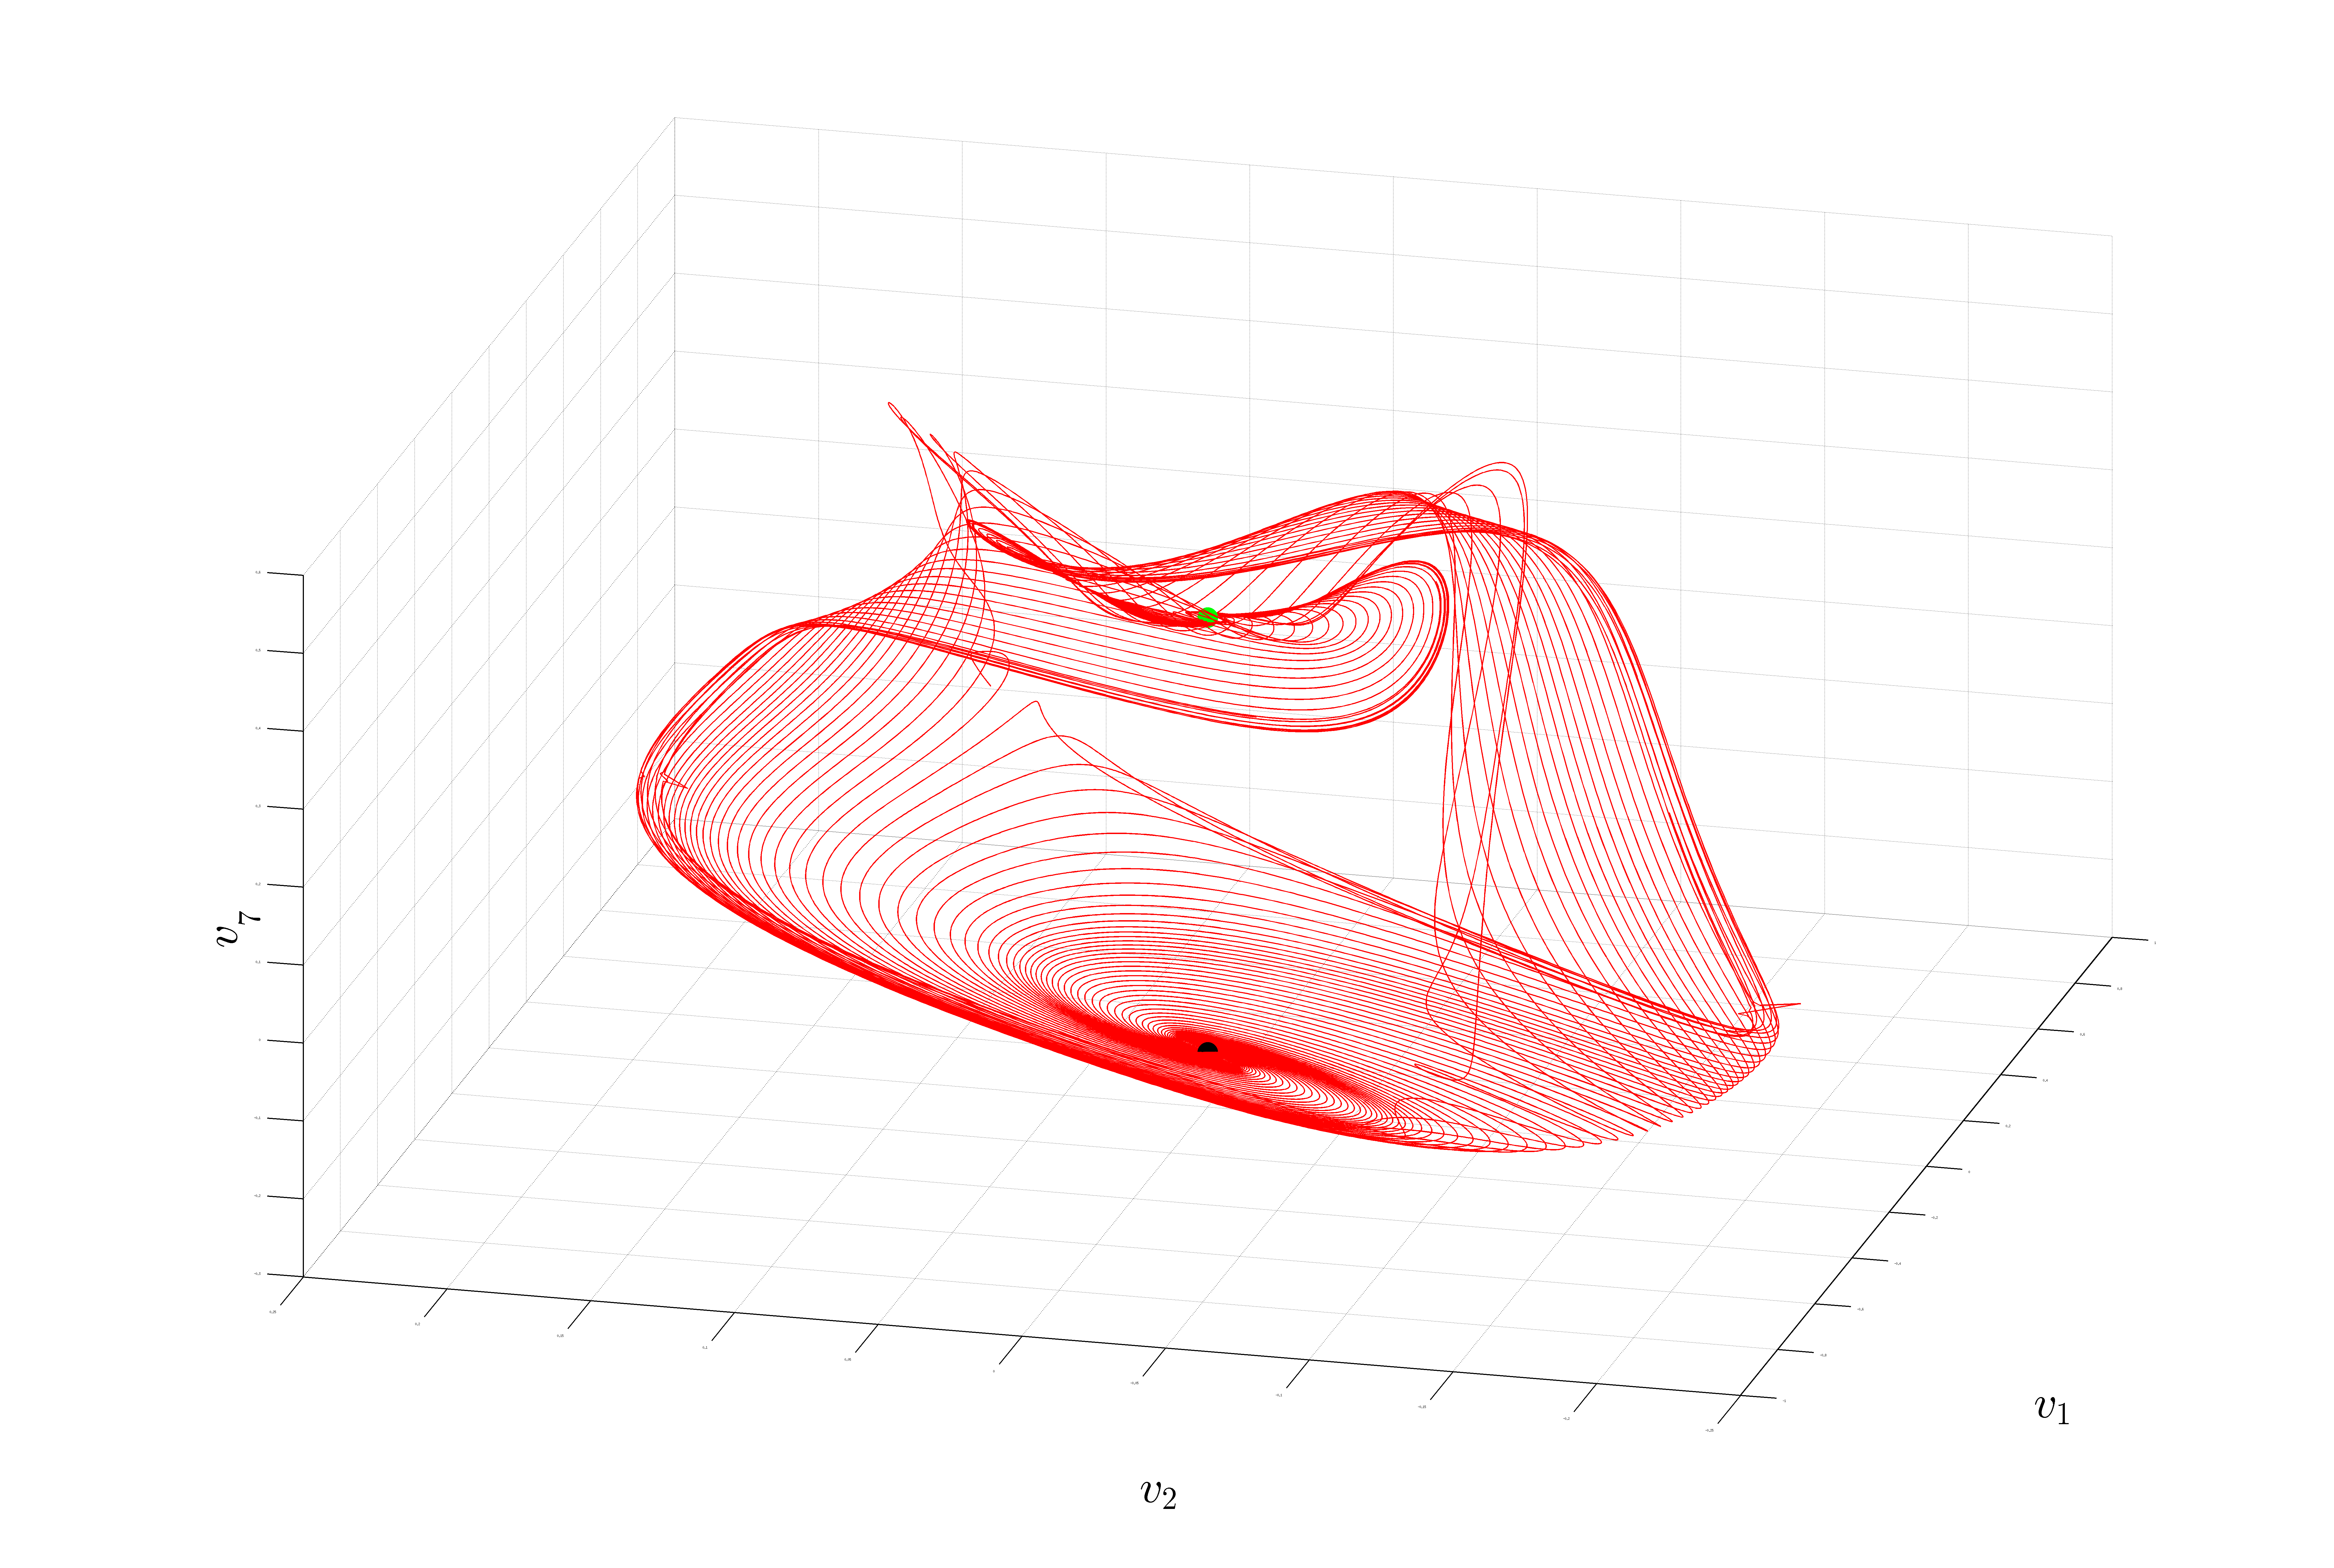
\includegraphics[width = 0.8\textwidth]{ks22_e2manifold}
  \caption{Unstable manifold of $E_2$, axes $v_1$, $v_2$ and $v_7$ are the
    real, imaginary part of first eigenvector and the real part of the
    seventh eigenvector. Black dot is $E_2$. Green dot is $\tau_{1/4}E_2$.
    2nd mode slice is used here.
  }
  \label{fig:ks22_e2manifold}
\end{figure}

\item[2014-09-3 Evangelos to Xiong]
$E_2$ and $\tau_{1/4}E_2$ representatives are there even if you do not implement symmetry
reduction at all (see e.g. our paper\rf{SCD07}). The $\pi$-unwrapping anticipates some descrete symmetry
and indeed can be thought of as a loose definition of the slice. I am not sure it's a 'legal' trick.
Anyway, the same result can be achieved by rotating the unstable manfold as a whole (there is no
motion in the direction of translations for trajectories on this manifold). Regarding the rpos that only
close after $2T_p$, this is a descrete symmetry induced by the 2nd mode slice. We have seen this
also in 2-modes system, and there has been a long discussion between me and Francesco in emails about this
(I will have to transfer it here). It would be nice to look in the slice equation in order to see where this
symmetry comes from.

What I see in your figure \ref{fig:ks22_e2manifold} and it worries me, are some kinks on the unstable manifold.
Do you know where they come from?

\item[2014-09-03 Xiong to Evanglos]
What I understand about the 2nd mode slice is
that each point will have 2 representatives on the slice if $2\pi$ phase
wrapping is implemented and 4 representatives on the slice if $\pi$ phase
is used. I just hope to check whether the unstable manifold of $E_2$
captures the majority of an ergodic trajectory, so a symbolic dynamics
could be built there. But now it seems that $TW_1$ is also important
in trapping trajectories. I am not sure.

For the kinks, If you are referring to the left upper
edge of \ref{fig:ks22_e2manifold}. I think it comes from the viewing
angle since the figure is symmetric. For other kinks in
\ref{fig:ks22_e2manifold2} (like the one at the left lower part), they
come from the group transform error when the orbit is close to the
{\sliceBord}.

\begin{figure}[h]
  \centering
  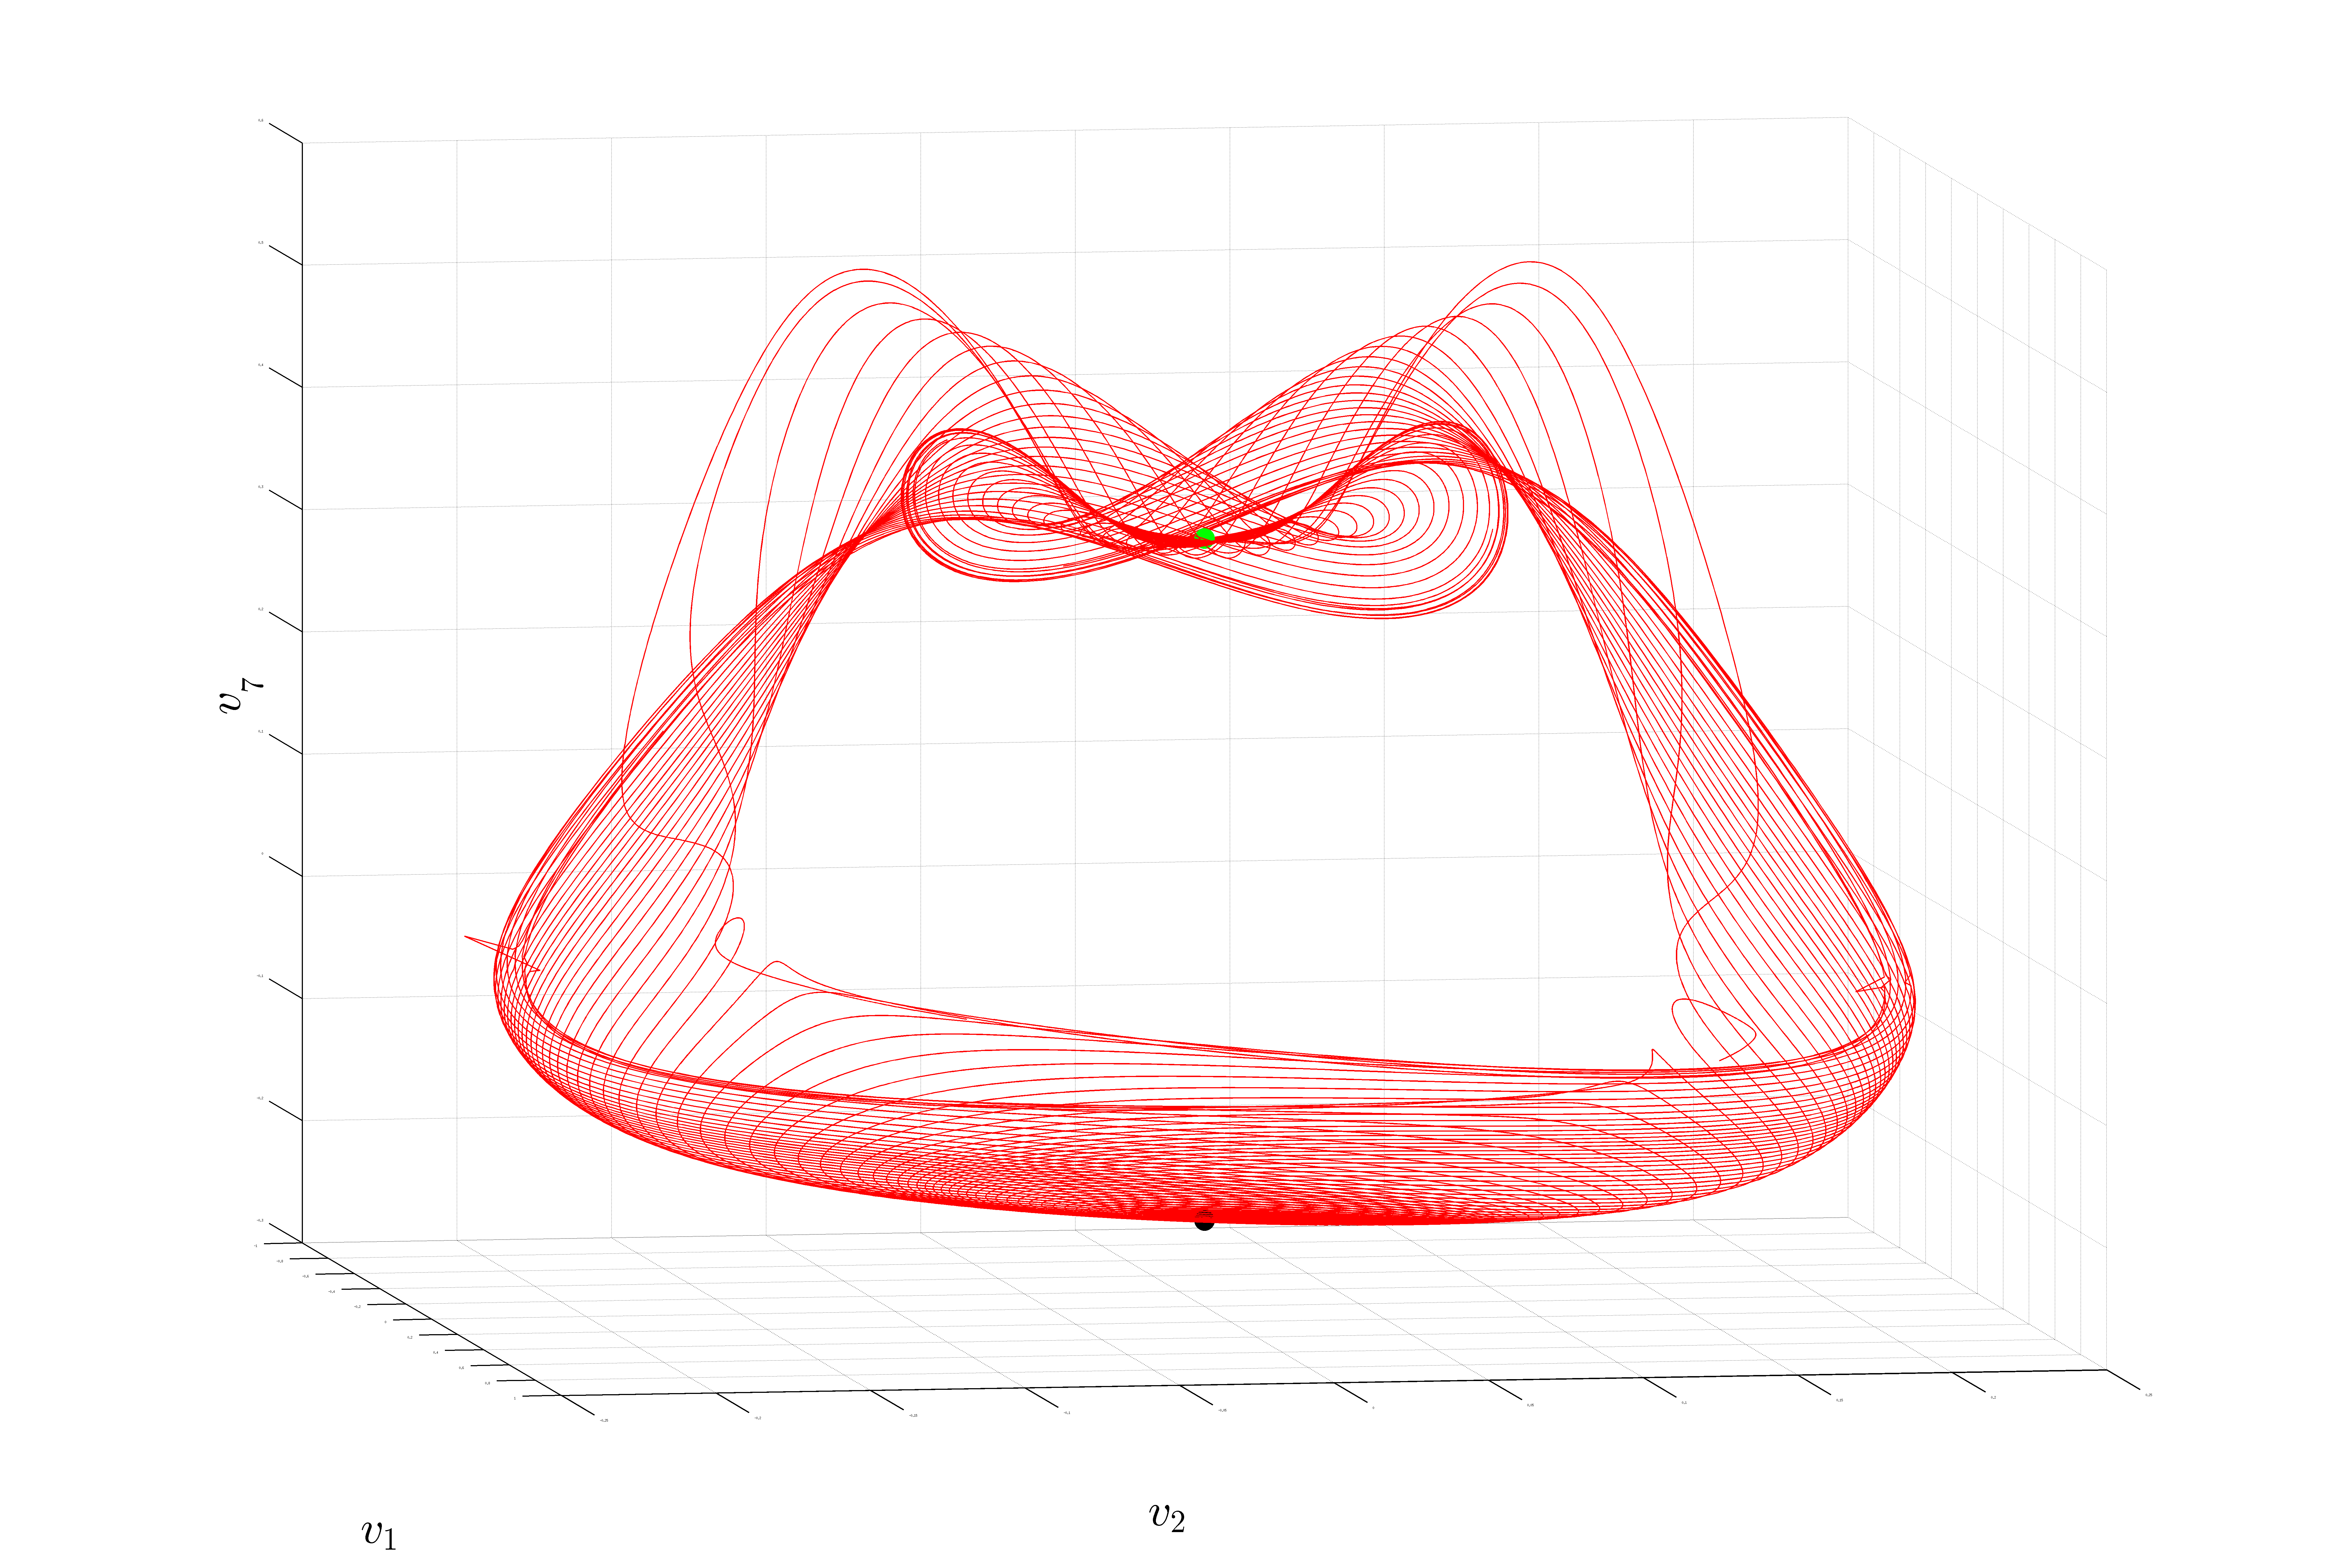
\includegraphics[width = 0.8\textwidth]{ks22_e2manifold2}
  \caption{ The same as \ref{fig:ks22_e2manifold}
  }
  \label{fig:ks22_e2manifold2}
\end{figure}

\item[2014-09-03 Evangelos to Xiong] My intention with the $\pi$ phase unwrapping was to
have fewer representatives of each point. Did I miss this goal completely, then?

I was referring to the kinks in the lower left and lower right part of \reffig{fig:ks22_e2manifold2}. Be careful because
if you see such kinks it could mean that you do not track angle correctly and your solution jumps.
For relative periodic orbits this is important, because then you might find they do not close when
they should.

Regarding organization of trajectories: the unstable manifold of $E_2$ certainly plays a role in
organizing trajectories, and that's why it's so important to get symmetry reduction 'close to it'
correctly. You can already see this in ergodic trajectories plots in physical space. This seems to be the
case if you look at phase space. For now the only figures I have produced are in ksReduced/obsolete/ksReduced.tex,
see Fig. 2.
In the same file you can also see that unstable manifold of $TW_1$ maybe also plays a role (Fig. 3), but it would be difficult
to use it for a return map. A better bet would be to try to use the unstable manifold of rpo with $T_p=16$.
I started doing this in Fig. 1 of that draft. In 2D projection it's hard to see, but shadowing orbits seem to
be organized by this unstable manifold.

\item[2014-02-08, 2014-10-04 Predrag] The rescaled time
\refeq{eq:scaledtime} is fine for numerical integrations. But I had hoped
also for coordinate rescaling that would replace the wild large radius
rotations by $\pi$ in \reffig{fig:BBKSmovframes} and in the \twomode\
model by straight lines crossing close to the `origin', as in the sketch
of the \HREF{http://www.youtube.com/watch?v=jkNJHfdZzHM} {homework
problem in a video format - click on it!} on rescaling. To spell it out
again: in the \SOn{2}-\reducedsp\ the coordinates are
\[
\hat{x} = (\hat{x}_1,0, \hat{x}_2, \hat{y}_2, \hat{x}_3 , \hat{y}_3, \cdots)
\,.
\]
When $\hat{x}_1$ is small, in each Fourier mode plane the trajectory
moves rapidly near the wall on a semicircle and renters increasing
$\hat{x}_1$ motion. Lets contract this semicircle by defining new
coordinates (keeping all the hats, so we remember we are still in the
\reducedsp),
\beq
\left[
\begin{array}{c}
\hat{p}_k  \\
\hat{q}_k
\end{array}
\right]
    =
\frac{\hat{x}_1}{\hat{r}_k}
\left[
\begin{array}{c}
\hat{x}_k  \\
\hat{y}_k
\end{array}
\right]
    \,,\qquad
\hat{r}_k = \left(\hat{x}_k^2 + \hat{y}_k^2 \right)^{1/2}
    \,,\qquad
k=2,3,\cdots
\,.
\ee{PCcoordinates}
This replaces $(\hat{p}_k , \hat{q}_k)$ dynamics by motion on the unit
circle $(\hat{p}_k/\hat{r}_k,\hat{q}_k/\hat{r}_k)$, rescaled by the
distance from the {\sliceBord}. Close to the vanishing first Fourier mode
$\hat{r}_k \to 0$, the trajectory
\(
(\hat{p}_k , \hat{q}_k) \approx \hat{x}_1 (\cos\phi,\sin\phi)
\,,
\)
traverses a vanishing neighborhood of the origin on trajectory segment of
length $\approx \hat{x}_1$ there are no wild jumps, and the transformed
coordinates  scale as length, so nothing is unnaturally scrunched, just
as advertised in my video.

Can you replot a few \twomode\ model and \KS\ plots in these coordinates?
If we like them, we can rewrite the equations in these coordinates, the
Jacobian of the transformation is straightforward.

\item[2014-10-21 Burak] I just plotted \twomode\ solutions using Predrag's
coordinates \refeq{PCcoordinates}, see \reffig{f-2modeSymmRedPredrag}.

\begin{figure}[h]
  \centering
  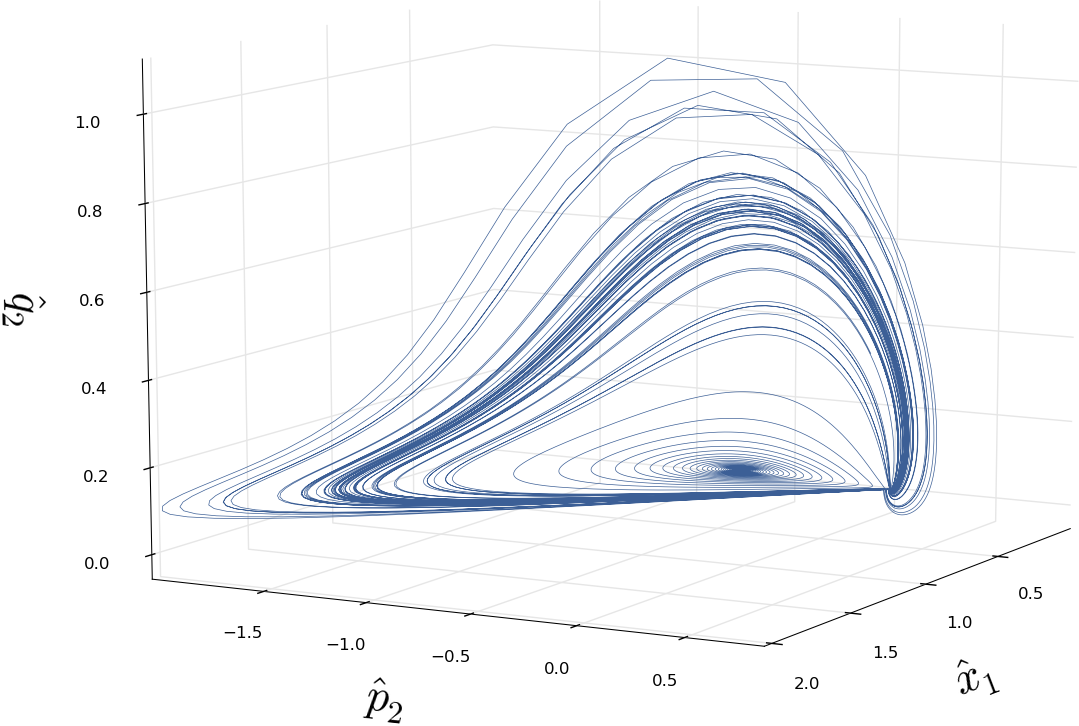
\includegraphics[width = 0.6\textwidth]{2modeSymmRedPredrag}
  \caption{\twoMode\ flow projected onto the coordinates given by
         \refeq{PCcoordinates}.}
  \label{f-2modeSymmRedPredrag}
\end{figure}

\item[2014-10-5 Evangelos to Predrag] I didn't realize this before, because I cannot watch
physics in youtube, I get distracted. The transformation that you propose is similar to
the one used in \reffig{f:ks22_E2_manifold_slice1_rpo4764_ip}, see [2014-06-29 Evangelos]
above. The difference is that you also divide by $\hat{r}_k$ (for `dimensional' consistency, I guess).
However, I am afraid that this will introduce similar problems when each of the $\tilde{r}_k$'s goes to zero.
This can be avoided by using $\hat{r}=\sqrt{\sum_{i=1}^{N}\left(\hat{x}_k^2 + \hat{y}_k^2\right)}$ instead of $r_k$.
This is one of the things that I tried in my thesis\rf{SiminosThesis}
(there is no figure, but it is explained\ES{Not really explained. My writing of that period was terrible, sorry.}
in the text).

In either case, the drawback of multiplying reduced variables by $\hat{x}_1$ is that any state space point with $\hat{x}_1=0$
is mapped to the origin. For KS this is a problem because equilibria $E_2$ and $E_3$ would become the same point
in reduced space. To overcome this problem, I used one more transformation to a more complicated set of invariant variables.
For 2-modes this degeneracy will not really be a problem, and maybe also for pipe flow.

I will replot \reffig{f:ks22_E2_manifold_slice1_rpo4764_ip} in \refeq{PCcoordinates}
and also in `thesis' coordinates $\hat{r}_k\rightarrow\hat{r}$ once I have access
to matlab tomorrow morning.

\item[2014-10-06 Predrag] I agree that my homework solution falls
short - I've gone to polar coordinates, and this takes care only of
angle, so I've thrown half coordinates out. No good. Need to design
something that keeps dependence on both the modulus and the phase, is
dimensionally a 'length', goes linearly to zero as one approaches the
{\sliceBord}. As in the first Fourier mode slice phase velocity has a
Dirac delta singularity at the wall, maybe we need to take a half-contour
in the complex plane, define 'principal part' when integrating the
trajectory. Or subtract the singularity. Dunno - will think again.
\end{description}
